\documentclass[10pt]{article}
\usepackage{commands}
\usepackage{slashed}
% \usepackage{pxfonts}
\pgfplotsset{compat=1.18}
\newcommand{\ddpd}[2]{\frac{\partial #1}{\partial #2}}
\newcommand{\diag}{\text{diag}}

\begin{document}
\begin{tcolorbox}
  \begin{center}
  \begin{Large}
    \textbf{PHYS 323 (Advanced Electrodynamics II) Notes} \\
    \vspace{5pt}
  \end{Large}
  \begin{large}
        Rio Weil \\
\vspace{5pt}
    \emph{This document was typeset on \today}
  \end{large}
  \end{center}
\end{tcolorbox}

\begin{center}
  \textbf{Introduction:}

  This is a set of lecture notes taken from UChicago's PHYS 323 (Advanced Electrodynamics II), taught by David Kutasov. Topics covered include...
\end{center}
\addtocontents{toc}{\protect\hypertarget{toc}{}}
\tableofcontents

\newpage
\section{Relativistic Kinematics}
Course logistics - see syllabus.

\subsection{Symmetries of Classical Mechanics}
We will start with Ch. 8/9 of Wald's book, and discuss relativistic kinematics.

The basic fact discovered after the formulation of Maxwell's theory of electromagnetism is that there is a clash between Maxwell's theory (Lorentz invariance) and the symmetries of classical mechanics (Galilean invariance). We will start by reviewing these symmetries, and then discuss how to promote these symmetries to field theory.

Consider the following (relatively general) class of problems. We have $N$ particles, labelled by coordinates $\v{x}_1(t), \v{x}_2(t), \ldots, \v{x}_N(t)$, which have pairwise interactions that only depend on the particle separation $V_{ij}(\abs{\v{x}_i - \v{x}_j})$. In classical mechanics (as you learned two quarters ago), we use a Lagrangian to describe the system:
\begin{equation}
    \LL = \frac{1}{2}\sum_{i=1}^N m_i \dot{\v{x}}^2_i - \sum_{i < j}V_{ij}(\abs{\v{x}_i - \v{x}_j})
\end{equation}
and we have the Euler-Lagrange equation(s) which are the equations of motion of the system:
\begin{equation}
    m_i\ddot{\v{x}}_i = -\nabla_i\sum_{y\neq i} V_{ij}(\abs{\v{x}_i - \v{x}_j})
\end{equation}
where we work in 3-dimensions, so $\v{x}_i = (x_i, y_i, z_i)$ and $\nabla_i = (\dpd{}{x_i}, \dpd{}{y_i}, \dpd{}{z_i})$. This theory has a couple symmetries (i.e. if we have a solution to the equations of motion, under some transformation the equations are still solutions. This manifests as a transformation that leaves $\LL$ invariant):
\begin{enumerate}
    \item Translational invariance:
    \begin{equation}
        \v{x}_i \to \v{x}_i + \v{a}
    \end{equation}
    The kinetic term does not change because the $\v{a}$ is not time-dependent (and hence is killed by the time derivative) and the potential term does not change because the potential only depends on the difference of the positions (and hence the $\v{a}$s cancel). Physically, we can take our entire system and shift it over by $\v{a}$ and nothing changes. Why are we wasting our time with this nonsense? Thanks to Noether, we know that this symmetry that looks nontrivial implies \emph{momentum conservation}.
    \item Time translation invariance:
    \begin{equation}
        t \to t + t_0
    \end{equation}
    Again, we see that this is a symmetry of $\LL$ because there is no explicit time-dependence in the Lagrangian. Noether tells us that this implies \emph{energy conservation}.
    \item Rotational invariance:
    \begin{equation}
        \v{x}_i \to R\v{x}_i
    \end{equation}
    for a rotation matrix $R$, i.e. that satisfying $RR^t = R^tR = \II$. The origin of this symmetry is that there is no preferred direction in space. Noether tells us that this implies \emph{angular momentum conservation}.
    \item Boost invariance:
    \begin{equation}
        \v{x}_i \to \v{x}_i - \v{v}t
    \end{equation}
    The previous 3 symmetries seem so robust that it seems like things cannot go wrong. Indeed, it is this fourth symmetry that must be modified when we consider the Maxwell theory. What this symmetry means is if we take the entire system and put it on a train going on a constant velocity relative to us, the physics of the system look the same (e.g. if we take the solar system and put it on a galactic train, the motion of the planets are left invariant).
\end{enumerate}
What about other transformations that depend on time? For example a transformation that depends on $t^2$? This would not be a symmetry - indeed we can feel if we are in an airplane and we are accelerating. This leads to the notion of an inertial frame. If we have some frame in which Newton's equations are valid, then any other frame that differs from our original frame via a boost will also be inertial. But accelerating frames are not inertial.

\subsection{Symmetry Group, Invariants of Classical Mechanics}
The symmetry group describing the symmetries of classical mechanics is the Galilean group. It is 10-dimensional; there are:
\begin{itemize}
    \item 3 spatial translation symmetries
    \item 1 time translation symmetry
    \item 3 rotation symmetries
    \item 3 boost symmetries
\end{itemize}
Side note - people like to divide the Galilean group into the homogenous Galilean group (rotations and boosts - which map coordinates under linear combinations of coordinates) and the inhomogenous Galilean group (space and time translations).

Consider two points in space + time - $(t_1, \v{x}_1), (t_2, \v{x}_2)$ (say, what time your alarm clock went off and what time you got out of bed). What combination of these coordinates are invariants?:
\begin{itemize}
    \item $\Delta t = t_2 - t_1$ is invariant under all of the above transformations.
    \item $\Delta x = \abs{\v{x}_2 - \v{x}_2}$ - is not invariant under boosts, as under $\v{x}' = \v{x} - \v{v}t$ we have:
    \begin{equation}
        \abs{\v{x}_2' - \v{x}_1'} = \abs{(\v{x}_2 - \v{v}t_2) - (\v{x}_1 - \v{v}t_1)} = \abs{\v{x}_2 - \v{x}_1 - \v{v}(t_2 - t_1)} \neq \abs{\v{x}_2 - \v{x}_1}
    \end{equation}
    However, if $t_1 = t_2$ then it is indeed an invariant.
\end{itemize}

\subsection{Generalization to Fields}
We now think about how to generalize these symmetries to fields. Consider the wave equation, which you saw in PHYS 322:
\begin{equation}\label{eq:waveeq}
    \square \phi(\v{x}, t) \coloneqq (-\frac{1}{c^2}\p_t^2 + \nabla^2)\phi(\v{x}, t) = 0
\end{equation}
Actually, we don't need to go to Maxwell/electromagnetic theory to see this; the wave equation already appears in classical mechanics, e.g. to describe waves on guitar strings, water etc.

The solutions to the wave equation are:
\begin{equation}
    \phi(\v{x}, t) = Ce^{i\v{k} \cdot \v{x} - \omega t}, \quad \omega = c\abs{\v{k}}
\end{equation}
where $c$ is the speed of propagation in the medium and $C$ some arbitrary multiplicative constant. Let's consider again the symmetries of our discrete classical theory and see what the effects of the transformations are.
\begin{itemize}
    \item Translations: if we take $\v{x} \to \v{x} + \v{a}, t \to t + t_0$, then we have:
    \begin{equation}
        \phi(\v{x}, t) \to \phi(\v{x} + \v{a}, t + t_0) = Ce^{i\v{k} \cdot(\v{x} + \v{a}) - i\omega(t + t_0)} = Ce^{i\v{k} \cdot \v{a} - i\omega t_0}e^{i\v{k} \cdot \v{x} - i\omega t}
    \end{equation}
    The translation simply yields a multiplicative constant/phase which is yet another solution to the wave equation.
    \item With boosts the story is different. Taking $\v{x} \to \v{x} - \v{v}t$, we have:
    \begin{equation}
        \phi(\v{x}, t) \to \phi(\v{x} - \v{v}t, t) = e^{i\v{k} \cdot \v{x} - i(\omega + \v{k} \cdot \v{v})t}
    \end{equation}
    so we have a new $\omega'$:
    \begin{equation}
        \omega' = \omega + \v{k} \cdot \v{v}
    \end{equation}
    but we require that $\omega' = c\abs{\v{k}}$, and indeed this does not hold generally:
    \begin{equation}
        \omega + \v{k} \cdot \v{v} \neq c\abs{\v{k}}
    \end{equation}
    unless the $\v{k} \cdot \v{v}$ term vanishes, i.e. the boost is in a perpendicular direction to the direction of propagation of the wave. In other words, while monochromatic waves do map to monochromatic waves, they do not preserve the dispersion relation.
\end{itemize}

At its face this seems to be a paradox. How is this consistent with the fact that boosts are a symmetry of our classical theory? There was indeed something we hid here - for the wave equation to be valid, the medium needs to be at rest - Eq. \eqref{eq:waveeq} assumes that the medium is at rest, for example (though we could generalize to the case of a moving medium)

Let us restrict ourselves to 1-d for moment and think about this further. Then, the solutions to the wave equation become:
\begin{equation}
    \phi(x, t) = e^{ikx - i\omega t}
\end{equation}
with boosted solutions:
\begin{equation}
    \phi'(x, t) = \phi(x + vt, t) = e^{ikx - i(\omega + kv)t}
\end{equation}
so in the boosted frame, it looks like the waves are travelling at speed:
\begin{equation}
    V = \frac{\omega + kv}{k} = \frac{\omega}{k} + v = c + v
\end{equation}
so we can see the law of composition of velocities emerge.

\subsection{Symmetry actions in Maxwell theory}
When Maxwell theory was proposed, people that believed that the same discussion holds for electromagnetic waves. As a result they believed two things:
\begin{enumerate}
    \item There was an ``Ether'', a frame where the light waves were at rest, analogous to the frame in the previous example where the water waves were at rest.
    \item The speed of light depends on the frame of reference.
\end{enumerate}
Michelson wasted 2 decades of his life trying to measure this effect (at least he got a UChicago building named after him!) and after this sequence of failures, people realized that our understanding needed to be amended. Indeed, the discussion of classical waves we just went through is \emph{not} a feature of electromagnetism. The actual situation is that Maxwell's equations hold in all inertial frames, and the symmetry group of nature is still generated by translations, rotations, and boosts, but the action of boosts is different from the classical case.

As a first step towards generalizing the action, let us remind ourselves how rotations act on monochromatic plane waves. As previously mentioned, we obtain the rotated coordinates via acting on our coordinates with a 3x3 rotation matrix:
\begin{equation}
    \v{x}' = R\v{x}
\end{equation}
Looking at $\v{k} \cdot \v{x}$:
\begin{equation}
    \v{k} \cdot \v{x} = \m{k_x & k_y & k_z}\m{x \\ y \\ z}
\end{equation}
If we replace $\v{x}$ with $\v{x}' = R^t\v{x}$ we have:
\begin{equation}
    \m{k_x & k_y & k_z}R^t\m{x' \\ y' \\ z'}
\end{equation}
We then have the rotated wavenumber:
\begin{equation}
    \m{k_x' & k_y' & k_z'} = \m{k_x & k_y & k_z}R^t \implies \m{k_x' \\ k_y' \\ k_z'} = R^t\m{k_x \\ k_y \\ k_z}
\end{equation}

So - If $\phi(\v{x}, t)$ is a solution to the wave equation, then $\phi'(\v{x}, t)$ (i.e. the solution where each $\v{k}$ is mapped to $\v{k}' = R^t\v{k}$) is also a (different) solution of that equation, which satisfies $\phi'(\v{x}', t) = \phi(\v{x}, t)$. This is an exercise which you can go through at home by taking a general solution and fourier decomposing it and applying the above wavenumber argument to each fourier component.

Now, let's return back to boosts - if we want the wave equation to be invariant under boosts (which it was not using the original definition of boosts), the best way to proceed is the following. We go from a 3-d story to a 3+1-d story:
\begin{equation}
    x^\mu = (x^0, x^1, x^2, x^3) = (ct, x, y, z)
\end{equation}
Now, we want to generalize the rotations in 3-d space to the full 3+1-d spacetime.

In space, we have the line element:
\begin{equation}
    ds^2 = dx^i dx^i = dx^2 + dy^2 + dz^2
\end{equation}
where the length of a trajectory is given by (in the 2-d case where $y = y(x)$ so $dy = y'dx$):
\begin{equation}
    L = \int ds = \int dx \sqrt{1 + y'^2}
\end{equation}
$ds$ is rotationally invariant:
\begin{equation}
    ds^2 = dx^idx^i = dx'^i dx'^i
\end{equation}
i.e. if you rotate your frame the distance between two points does not change. This is the thing that we generalize to 3+1d. We define the line element:
\begin{equation}
    ds^2 = dx^\mu dx^\nu \eta_{\mu\nu} = -(dx^0)^2 + (dx^1)^2 + (dx^2)^2 + (dx^3)^2
\end{equation}
with $\eta_{\mu\nu}$ the Minkowski metric:
\begin{equation}
    \eta = \text{diag}(-1, 1, 1, 1).
\end{equation}

How does this help? Let's look at the wave equation. $\phi$ originally was a function of $\v{x}, t$, which we've repackaged into $x^\mu$:
\begin{equation}
    \square \phi(x^\mu) = 0, \quad \square = \frac{1}{c^2}\dpd[2]{}{t} + \frac{\partial}{\partial x^i}\frac{\partial}{\partial x^i} = -\p_0^2 + \p_i \p_i = \frac{\partial}{\partial x^\mu}\frac{\partial}{\partial x^\mu}\eta^{\mu\nu}
\end{equation}
An important note; previously, indices on coordinates were just an aesthetic choice. But here now one of the signs of the metric is different, so we need to take a little more care with where we put our indices. In particular, given $x^\mu$ we can define:
\begin{equation}
    x_\mu = \eta_{\mu\nu}x^\nu
\end{equation}
so:
\begin{equation}
    x_0 = -x^0, x_i = x^i
\end{equation}
Note that this implies that $\frac{\partial}{\partial x^\mu}$ actually carries a lower index. $x^\mu x_\mu$ is Lorentz invariant (note the Einstein summation convention/repeated indices are summed over), and taking its derivative:
\begin{equation}
    \frac{\partial}{\partial x^\mu}(x^\nu x_\nu) = 2x_\mu
\end{equation}
so since taking the derivative results in an object with a lower index, $\frac{\partial}{\partial x^\mu}$ indeed carries a lower index. This motivates the $\frac{\partial}{\partial x^\mu}\frac{\partial}{\partial x^\mu}\eta^{\mu\nu}$ we wrote in the D'Alambertian.

Note that fortunately, the metric with upper indices is identical to the metric with lower indices:
\begin{equation}
    \eta_{00} = -1, \quad \eta_0^{\sp 0} = +1 \implies \eta^{00} = -1
\end{equation}

This discussion was a bit fast, but we will continue it next class. It's recommended that you read the relevant sections in Wald to refresh yourself on all of this index manipulation.
\section{Lorentz Transformations}

\subsection{Review of last class}
Last time, we were discussing the question of how pre-relativistic spacetime symmetries can be promoted to be consistent with the Maxwell theory. We generalized from rotations; we have three space coordinates $(x^1, x^2, x^3) = (x, y, z)$ and the line element:
\begin{equation}
    ds^2 = dx^2 + dy^2 + dz^2 = dx^idx^i
\end{equation}
where the summation over the repeated index $i$ is implied. Rotations have the action on the coordinates:
\begin{equation}
    x'^i = R^i_j x^j
\end{equation}
with $R^tR = RR^t = \II$. The line element $ds^2$ is invariant under rotations:
\begin{equation}
    ds'^2 = dx'^i dx'^i = dx^i dx^i = ds^2
\end{equation}
The idea is that given two points $\v{x}_1, \v{x}_2$, the squared distance:
\begin{equation}
    D^2 = \abs{\v{x}_2 - \v{x}_1}^2
\end{equation}
is invariant under rotations. For our purpose, it is also useful to recall that $\nabla^2 = \p_i \p_i$ is also invariant:
\begin{equation}
    \nabla'^2 = \ddpd{}{x'^i}\ddpd{}{x'^i} = \nabla^2
\end{equation}
The idea was to now include time:
\begin{equation}
    ds^2 = -(dx^0)^2 + (dx^1)^2 + (dx^2)^2 + (dx^3)^2 = dx^\mu dx^\nu \eta_{\mu\nu}
\end{equation}
with $x^0 = ct$, and $\mu, \nu = 0, 1, 2, 3$ and:
\begin{equation}
    \eta_{\mu\nu} = \text{diag}(-1, 1, 1, 1).
\end{equation}
Note that we can write the line element equivalently as:
\begin{equation}
    ds^2 = dx^\mu dx_\mu
\end{equation}
where:
\begin{equation}
    dx_\mu = \eta_{\mu\nu}dx^\nu
\end{equation}
generally, we are able to lower any index using the spacetime metric (here a metric on $R^{1, 3}$). With this definition, note:
\begin{equation}
    dx_0 = -dx^0, \quad dx_i = dx^i
\end{equation}
Note that greek indices run over all 4 spacetime components, while alphabetic indices $(i, j, k)$ only run over spatial.

\subsection{Spacetime Intervals and Poincare Symmetry}
For two points in spacetime $x^\mu, y^\mu$, we can define the spacetime interval:
\begin{equation}
    I = -(x^\mu - y^\mu)(x^\nu - y^\nu)\eta_{\mu\nu} = -(x^0 - y^0)^2 + \abs{\v{x} - \v{y}}^2
\end{equation}
There are three cases:
\begin{itemize}
    \item For $I > 0$, $x, y$ are spacelike separated.
    \item For $I < 0$, $x, y$ are timelike separated.
    \item For $I = 0$, $x, y$ are lightlike separated.
\end{itemize}
$I$ behaves like an inner product of sorts on spacetime, but it is not positive definite.

Note that $ds^2$ is invariant under transformations of the form:
\begin{equation}
    x'^\mu = \Lambda^{\mu}_{\sp\nu}x^\nu
\end{equation}
It is very important to get the location of indices correct!\footnote{If you wrote the LHS as $x'_\mu$ on the midterm, the grader is going to be in pain.}

$\Lambda$ satisfies:
\begin{equation}
    \Lambda^\mu_{\sp\lambda}\Lambda^{\nu}_{\sp\rho}\eta_{\mu\nu} = \eta_{\lambda\rho}
\end{equation}

\subsection{Solutions to the Wave Equation}

Recall the box operator, which we can now write compactly:
\begin{equation}
    \square = -\frac{1}{c^2}\p_t^2  +\nabla^2 = \p_\mu \p^\mu = \p_\mu \p_\nu \eta^{\mu\nu}
\end{equation}
Like the Laplacian was invariant under rotations, the box operator is invariant under Lorentz transformations/$\Lambda$s:
\begin{equation}
    \square_x = \square_{x'}
\end{equation}

What do we learn from this? If $\phi(x^\mu)$ is a solution of the wave equation:
\begin{equation}
    \square_x \phi(x) = 0
\end{equation}
then $\phi'(x)$ is also a solution of the wave equation. $\phi'$ is defined by:
\begin{equation}
    \phi'(x') = \phi(x)
\end{equation}

An important example is plane waves:
\begin{equation}
    \phi(x^\mu) = e^{ik_\mu x6\mu} = e^{ik^\mu x^\nu \eta_{\mu\nu}}
\end{equation}
Note that if $\phi$ is a solution:
\begin{equation}
    \box \phi(x^\mu) = ik^\mu ik_\mu e^{ik^\mu x_\mu} = 0
\end{equation}
thus:
\begin{equation}
    k^\mu k_\mu = 0 \implies (k^0)^2 = \abs{\v{k}}^2 \implies k^0 = \abs{\v{k}}
\end{equation}
where we take the positive root. In the discussion we had on Tuesday, we quoted the familiar result from last quarter:
\begin{equation}
    \phi(\v{x}, t) = e^{-i\omega t + i\v{k} \cdot \v{x}}
\end{equation}
with $\omega = c\abs{\v{k}}$. This condition is exactly the same as that we write above:
\begin{equation}
    \phi(\v{x}, t) = e^{-i\omega t + i\v{k} \cdot \v{x}} = e^{-i\frac{\omega}{c}x^0 + i\v{k} \cdot \v{x}} = e^{-ik^0 x^0 + i\v{k}\cdot\v{x}}
\end{equation}
So if we substitute $k^0$ into the dispersion relation:
\begin{equation}
    k^0 = \abs{\v{k}}.
\end{equation}

For this $\phi(x)$, $\phi'(x)$ looks like:
\begin{equation}
    e^{ik_\mu' x^\mu}
\end{equation}
where:
\begin{equation}
    k_\mu' = \Lambda_{\mu}^{\sp\nu}k_\nu
\end{equation}
Note that in order for this be a solution, we must have that the $k$s are lightlike, as they are for the original solution:
\begin{equation}
    k'^\mu k'_\mu = 0
\end{equation}
But this is guaranteed by the fact that the Lorentz transformations preserve the metric (check it if you aren't convinced).

Last class we had the problem that applying a boost to a solution of the wave equation was not a solution - we have now fixed this.

\subsection{Lorentz Transformations - Rotations and Boosts}
There is a special class of Lorentz transformations where $\Lambda_0^{\sp0} = 1$ and $\Lambda_0^{\sp i} = 0$, which look like:

\begin{equation}
    \Lambda = \m{1 & 0 & 0 & 0 \\ 0 & & & \\ 0 & & R & \\ 0 & & &}
\end{equation}

Note that for these:
\begin{equation}
    x'^0 = \Lambda^0_{\sp \nu}x^\nu = x^0
\end{equation}
\begin{equation}
    x'^i = \Lambda^{i}_{\sp\nu}x^\nu = R^i_j x^j
\end{equation}
for $R^t R = RR^t = \II$, so rotations are just a subclass of Lorentz transformations. Given that rotations of solutions to the wave equation are also solution, this is not too surprising.

A couple examples; for a rotation about the $z$-axis by the angle $\theta$:
\begin{center}
    \begin{center}
        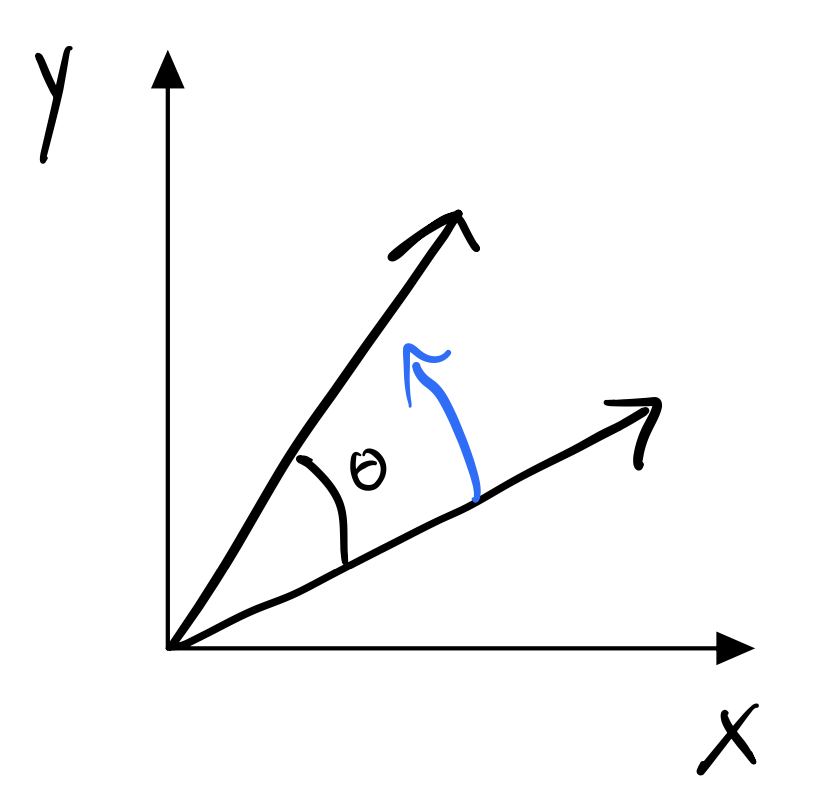
\includegraphics[scale=0.35]{Lectures/Images/lec2-rotation.png}
    \end{center}
    
\end{center}
we have:
\begin{equation}
    R = \m{\cos\theta & -\sin\theta & 0 \\ \sin\theta & \cos\theta & 0 \\ 0 & 0 & 1}
\end{equation}

For a boost in the $x'$ direction with velocity $v$, we have:
\begin{equation}
    \Lambda_{\mu}^{\sp\nu} = \m{\gamma & -\beta \gamma & 0 & 0 \\ -\beta \gamma & \gamma & 0 & 0 \\ 0 & 0 & 1 & 0 \\ 0 & 0 & 0 & 1}
\end{equation}
where the parameters obey (in order for $\Lambda$ to preserve the metric):
\begin{equation}
    \gamma^2(1 - \beta^2) = 1
\end{equation}
$\beta = \frac{v}{c} \in (-1, 1)$ as nothing travels faster than the speed of light. Rearranging for $\gamma$, we have the familiar expression:
\begin{equation}
    \gamma = \frac{1}{\sqrt{1 - \beta^2}}
\end{equation}

We can write:
\begin{equation}
    \beta = \tanh\zeta
\end{equation}
where $\zeta \in (-\infty, \infty)$ is the rapidity. In this parameterization:
\begin{equation}
    \gamma = \frac{1}{\sqrt{1-\beta^2}} = \frac{1}{\sqrt{1 - \tanh^2\zeta}} = \cosh\zeta
\end{equation}
where we have used $\cosh^2\zeta = \sinh^2\zeta + 1$. Note then that $\beta\gamma = \sinh\zeta$. So we can write the boost transformation as:
\begin{equation}
    \Lambda = \m{\cosh\zeta & -\sinh\zeta & 0 & 0 \\ -\sinh\zeta & \cosh\zeta & 0 & 0 \\ 0 & 0 & 1 & 0 \\ 0 & 0 & 0 & 1}
\end{equation}
Which looks quite analogous to what we had with the spatial rotations, except we have replaced the trigonometric functions with their hyperbolic counterparts. Indeed, we can view boosts as hyperbolic rotations.

Under a boost, we have:
\begin{equation}
    \m{x'^0 \\ x'^1} = \m{\gamma & -\beta\gamma \\ -\beta\gamma & \gamma}\m{x^0 \\ x^1} = \m{\gamma x^0 - \beta\gamma x^1 \\ \gamma x^1 - \beta\gamma x^0}
\end{equation}
In the nonrelativistic limit of $v/c \ll 1$:
\begin{equation}
    \gamma = (1-\beta^2)^{-\frac{1}{2}} \approx 1 + \frac{1}{2}\beta^2
\end{equation}
so:
\begin{equation}
    x'0 \approx x^0, \quad x'^1 = x' - \frac{v}{c}\cdot c t
\end{equation}
so we recover the expressions for old (Galilean) boosts. So classical physics was not wrong per se, it just emerges as the nonrelativistic limit of the correction theory. But when we look at relativistic physics (e.g. electromagnetic waves, high-energy particle scattering...) we need to use the relativistic theory.

On Tuesday, we discussed the 10 dimensional Galilean group which quantified the symmetry of classical mechanics. Now, we have modified boosts (i.e. the homogenous part of the Galilean group). The group consisting of 3 spatial rotations + 3 relativistic boosts yields the 6-dimensional Lorentz group, and the 4 spacetime translations yields the 10-dimensional Poincare group.

\subsection{Doppler Effect}
Recall the monochromatic wave solution:
\begin{equation}
    \phi = e^{ik_\mu x^\mu}
\end{equation}
with:
\begin{equation}
    k^2 = k_\mu k^\mu = 0
\end{equation}
\begin{equation}
    \omega = ck^0 = ck, \quad \v{k} = \hat{\v{k}}k = \hat{\v{k}}\frac{2\pi}{\lambda}
\end{equation}
The two heroes of the story are the frequency and $\hat{\v{k}}$ the direction of propagation.

\begin{center}
    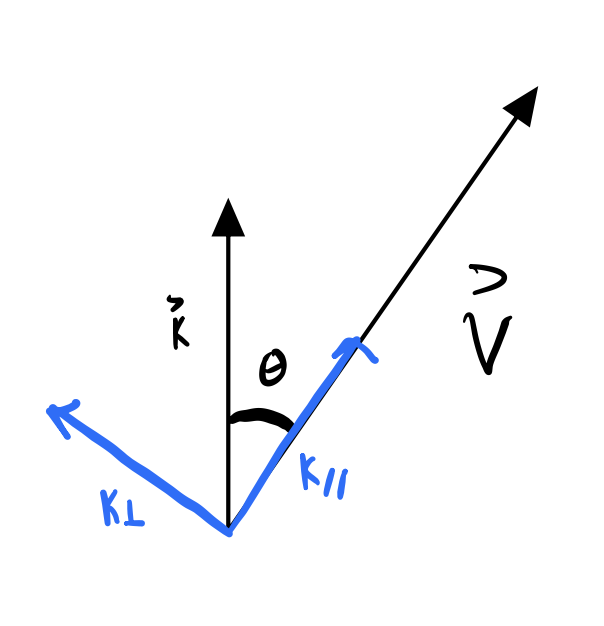
\includegraphics[scale=0.35]{Lectures/Images/lec2-wavevectorboost.png}
\end{center}

The question is now - what does a boosted observer see? We consider the wavevector $\v{k}$ and decompose it into the components perpendicular and parallel to the boost velocity. $\theta$ is the angle between the two vectors. Let us calculate:
\begin{equation}
    k'^\mu = \Lambda^{\mu}_{\sp\nu}k^\nu
\end{equation}
We have:
\begin{equation}
    k'^0 = \gamma(k^0 - \gv{\beta}\cdot\v{k}) = \gamma(k^0 - \beta k_\parallel)
\end{equation}
\begin{equation}
    k'_\parallel = \gamma(k_\parallel - \beta k^0)
\end{equation}
\begin{equation}
    \v{k}'_\perp = \v{k}_\perp
\end{equation}
the last equality follows from the fact that the $\Lambda$ matrix is trivial in this sector.

A good consistency check is that:
\begin{equation}
    k'^2 = k'_\mu k'^\mu = 0
\end{equation}
which you can verify. This tells us that the boosted observer still sees the EM wave propagating at speed:
\begin{equation}
    k'^0 = \abs{\v{k}'}
\end{equation}
This is not something to be surprised about - the formalism was built for this to be true.

If the speed of propagation is not different, what is different? Well, let's look at the $k'^0$ relation. We can write this as:
\begin{equation}
    \omega' = \gamma\omega(1 - \beta\cos\theta)
\end{equation}
So, we see a different frequency, which is the Doppler effect! The direction of propagation is also modified:
\begin{equation}
    \tan\theta = \frac{\abs{\v{k}_\perp}}{k_\parallel}, \quad \tan\theta' = \frac{\abs{\v{k}'_\perp}}{k'_\parallel} =  \frac{\abs{\v{k}_\perp}}{\gamma(k_\parallel - \beta k^0)}
\end{equation}
Since the denominator changes, so too must the angle.

Note the special case of the frequency relation when $\theta = \pi/2$, then:
\begin{equation}
    \omega' = \gamma\omega
\end{equation}
so the shift is manifestly relativistic.

\subsection{Teaser - Relativistic Formulation of Maxwell Theory}
You might say - hey, weren't we studying Maxwell theory the whole time? Indeed we were studying the wave equation, but there is more to Maxwell theory than this! We have to talk about two things:
\begin{itemize}
    \item The dynamics of (charged) particles in electromagnetic fields
    \item The dynamics of the electromagnetic field itself
\end{itemize}

Consider the Lorentz force; suppose we have particle with spatial coordinate $\v{x}(t)$ and charge $q$. In the presence of EM fields, the equation of motion is given by:
\begin{equation}
    \dod{(m\dot{\v{x}})}{t} = \dod{\v{p}}{t} = q(\v{E} + \v{v}\times\v{B})
\end{equation}
These equations are written in a highly inconvenient way for our purposes, as they treat time and space very differently. Time is a label and $\v{x}$ is the position of interest. But for us, we want to package things in terms of 4-vectors/spacetime coordinates $x^\mu = (x^0 = ct, \v{x})$. Thus the above formulation is very inconvenient, e.g., to see how Lorentz transformations work in this theory. We will see how we can formulate the Maxwell theory in a relativistically covariant fashion next time.
\section{Relativistic Formulation of a Free Particle}

At the end of last week, we discovered that the wave equation (in Maxwell theory) must hold in all inertial frames, and as such the notion of boosts in Maxwell theory is different from the Galilean version in classical mechanics. Today what we will do is follow Einstein, and take the attitude that all physical laws must be Lorentz invariance.

To this end, we will need to be generalize the idea of the coordinate $\v{x}(t)$. In classical mechanics, the momentum $\v{p} = m\dot{\v{x}}$ is conserved, and can take on any value. But in the relativistic theory $\abs{\dot{\v{x}}}$ is bounded above by the speed of light. Some kind of reformulation is necessary. We also have the EM fields $\v{E}(\v{x}, t), \v{B}(\v{x}, t)$ - these are already coming out of a Lorentz invariant theory, but we can rewrite the Maxwell equations such that they are manifestly Lorentz covariant.

\begin{center}
    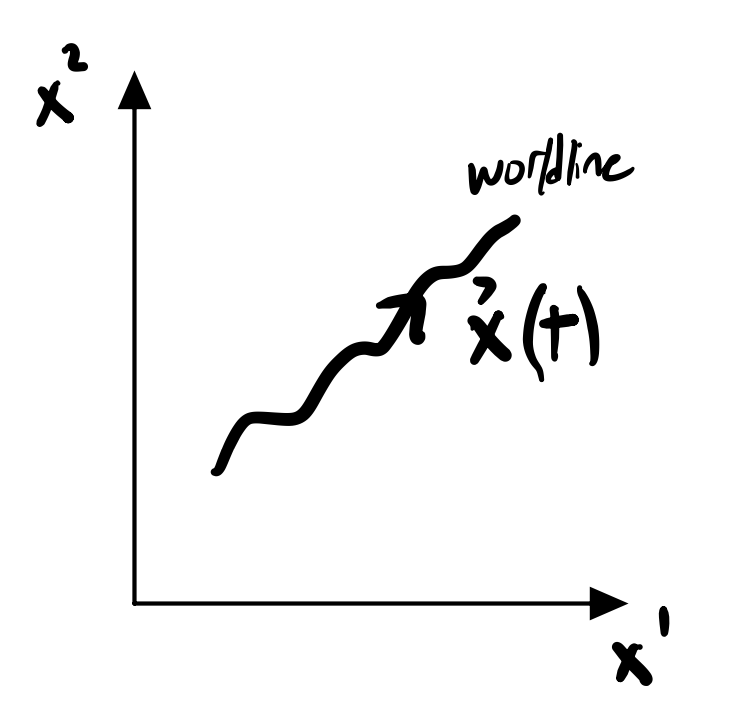
\includegraphics[scale=0.35]{Lectures/Images/lec3-worldline.png}
\end{center}

In classical mechanics, we write down the Lagrangian:
\begin{equation}
    \mathcal{L} = \frac{1}{2}m\dot{\v{x}}^2 - U(\v{x})
\end{equation}
and then solve the EL equations to find the trajectories. 

\subsection{Parametrization}
However, for a relativistically covariant formulation, we would like to put $\v{x}, t$ on the same footing. To this end, we can introduce a parameter $\lambda$, and describe the worldline of the particle as:
\begin{equation}
    x^\mu = x^\mu(\lambda)
\end{equation}
with $\mu = 0, 1, 2, 3$. This might look outlandish, but we do such parametrizations in simpler contexts. For example, consider a line in 2D space:

\begin{center}
    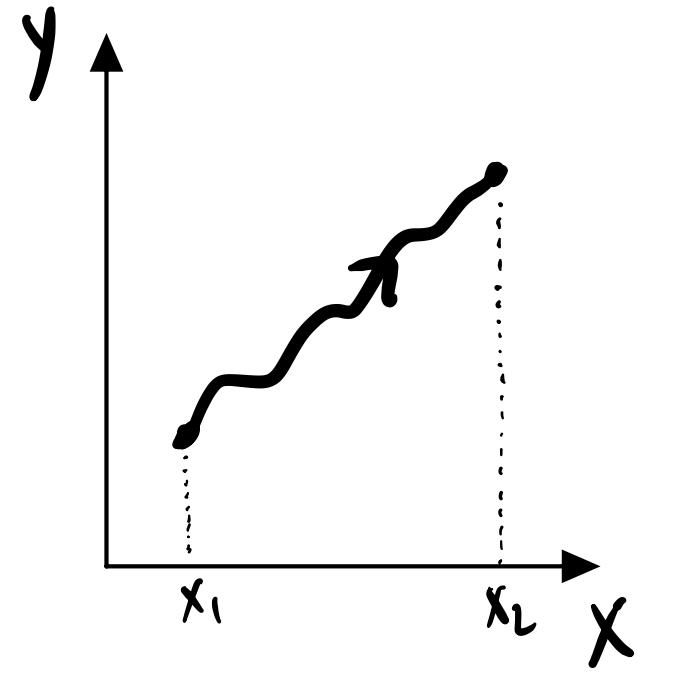
\includegraphics[scale=0.35]{Lectures/Images/lec3-yxpath.png}
\end{center}

Then we could either write $y = y(x)$, or we could write $y = y(\lambda), x = x(\lambda)$ and make them depend on a common parameter:
\begin{equation}
    x = \lambda, y = \lambda^2, \lambda \in [0, 1]
\end{equation}
In doing so, we actually introduced an additional symmetry in the form of reparametrization invariance; indeed we can have $x, y$ in terms of an arbitrary (monotonic, positive) function of $\lambda$:
\begin{equation}
    x= f(\lambda), y = f^2(\lambda), \lambda \in [0, 1]
\end{equation}
This can be useful for calculations in various contexts. For example, suppose we were interested in calculating the length of the line:

\begin{center}
    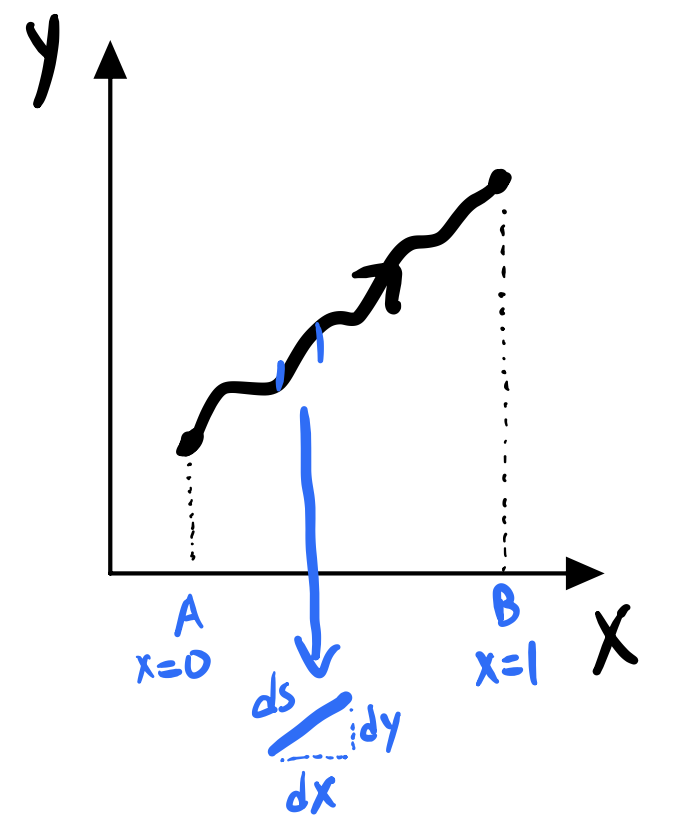
\includegraphics[scale=0.35]{Lectures/Images/lec3-lineelement.png}
\end{center}

Then:
\begin{equation}
    L = \int_A^B ds = \int_A^B \sqrt{dx^2 + dy^2} = \int_0^1 dx \sqrt{1 - \left(\dod[]{y}{x}\right)^2} = \int_0^1 dx\sqrt{1 + y'^2}
\end{equation}

But if $x = x(\lambda), y = y(\lambda)$ for some parameter $\lambda$, we could then write:
\begin{equation}
    ds^2 = (dx(\lambda))^2 + (dy(\lambda))^2 = \left(\dod{x}{\lambda}d\lambda\right)^2  + \left(\dod{y}{\lambda}d\lambda\right)^2 = d\lambda^2\left(\dot{x}^2 + \dot{y}^2\right)
\end{equation}
So:
\begin{equation}
    L = \int_A^B ds = \int_A^B \sqrt{d\lambda^2\left(\dot{x}^2 + \dot{y}^2\right)} = \int_A^B d\lambda\sqrt{\dot{x}^2 + \dot{y}^2}
\end{equation}
the length calculation is now symmetric in $x, y$. If we replace $\lambda \to f(\lambda)$, the length should not change (for it shouldn't matter on the parameterization of the curve!) This must be a symmetry of the integral, and indeed we can easily check that it is. Under $\lambda \to f(\lambda)$:
\begin{equation}
    x^\mu = \frac{dx^\mu}{d\lambda} \to \frac{dx^\mu}{df(\lambda)} = \frac{dx^\mu}{d\lambda}\frac{d\lambda}{df(\lambda)}
\end{equation}
and the same for $y^\mu$. Thus the length becomes:
\begin{equation}
    L = \int_A^B df(\lambda)\sqrt{\left(\frac{dx^\mu}{df(\lambda)}\right)^2 + \left(\frac{dy^\mu}{df(\lambda)}\right)^2} = \int_A^B d\lambda \dot{f} \sqrt{\left(\frac{\dot{x}}{\dot{f}}\right)^2 + \left(\frac{\dot{y}}{\dot{f}}\right)^2} = \int_A^B d\lambda\sqrt{\dot{x}^2 + \dot{y}^2}
\end{equation}
which we can see is invariant (as it should be).

\subsection{Parametrizing Worldlines and Time Dilation}
Back to our problem of parametrizing worldlines. We can repeat the idea from the simple context here, by describing the particle worldine as $x^\mu(\lambda)$. Other than the fact that the time component has a different sign:
\begin{equation}
    ds^2 = -(dx^0)^2 + (dx^1)^2 + (dx^2)^2 + (dx^3)^2
\end{equation}
we can play the same game as before; with $x^\mu = x^\mu(\lambda)$:
\begin{equation}
    ds^2 = d\lambda^2\left(-(\dot{x}^0)^2 + (\dot{x}^1)^2 + (\dot{x}^2)^2 + (\dot{x}^3)^2\right) = d\lambda^2 \dot{x}^\mu \dot{x}_\mu = d\lambda^2 \dot{x}^\mu \dot{x}^\nu \eta_{\mu\nu}
\end{equation}
This line element is reparametrization invariant, but also is Lorentz invariant (as it is written as a contraction with the Minkowski metric).

To do physics, we want to fix reparametrization symmetry. It is natural to fix $x^0(\lambda) = \lambda c$, so then $t(\lambda) = \lambda$. The logic is we have four functions, and we can freely reparametrize - using this symmetry, we may pick the time function to be simple. Let's see what happens to $ds^2$ when we do this:
\begin{equation}
    ds^2 = dt^2\left(-c^2 + \left(\dod{\v{x}}{t}\right)^2\right) = -c^2dt^2\left(1 - \gv{\beta}^2\right)
\end{equation}
with $\gv{\beta} = \frac{\v{v}}{c} = \frac{\dot{\v{x}}}{c}$. A natural definition is:
\begin{equation}
    d\tau^2 = dt^2(1 - \gv{\beta}^2)
\end{equation}
so:
\begin{equation}
    ds^2 = -c^2d\tau^2
\end{equation}
$\tau$ is called the proper time. In the frame where $\gv{\beta} = 0$, we can see from the above $\tau = t$; it thus has the interpretation as the time in the inertial frame in which the particle is at rest momentarily. The relation between $t, \tau$ can be written as:
\begin{equation}
    dt = \gamma d\tau
\end{equation}
with:
\begin{equation}
    \gamma^2 = \frac{1}{1 - \gv{\beta}^2}
\end{equation}
This is the celebrated time dilation formula. This says that things that take time $d\tau$ in the frame of the particle are dilated/increased by $\frac{1}{1-\gv{\beta}^2}$ in the frame of the external observer. As a concrete example, if a particle has a lifetime $T$, someone who sees the particle moving will see its lifetime as $\gamma T$. You may be familiar with the fact that cosmic rays create muons with, $T = 2.2 \cdot 10^{-6}\si{s}$. In the muon frame, it can only travel $2. 2 \cdot 10^{-6}\si{s} \cdot 3 \times 10^{8}\si{ms^{-1}} = 0.66\si{km}$. But we observe that cosmic ray muons propagate for hundreds of kilometers, and the explanation is that their lifetime is extended via time dilation.

\subsection{Lagrangian for Relativistic Particle}
The usual Lagrangian:
\begin{equation}
    \mathcal{L} = \frac{1}{2}m\dot{\v{x}}^2 - U(\v{x})
\end{equation}
does not work in our relativistic formulation as the particle could have any velocity, and velocities are bounded by the speed of light. Further, the action $S = \int dt \mathcal{L}$ is not invariant under Lorentz transformations. Can we modify this Lagrangian in some way? A very natural candidate is:
\begin{equation}\label{eq:LIaction}
    S = A\int d\lambda \sqrt{-\dot{x}_\mu \dot{x}^\mu}.
\end{equation}
This is automatically Lorentz invariant. It is also reparametrization invariant, so let us fix the reparametrization symmetry by taking $\lambda = t$:
\begin{equation}
    S = \tilde{A}\int dt \sqrt{1 - \frac{\dot{\v{x}^2}}{c^2}}.
\end{equation}
This is now invariant under the boosts that we defined last week - even though it looks like it mixes $x/t$ because they are written separately, we know from the form of Eq. \eqref{eq:LIaction} that it is indeed invariant. It is also now clear why we took the minus sign there; we want the argument of the square root to be always positive.

We are not quite done yet. We have to check that the action passes basic scrutiny. One sanity check is that in the non-relativistic limit of $\dot{\v{x}} \ll c$. Using the binomial approximation:
\begin{equation}
    S = \tilde{A}\int dt\left[1 - \frac{1}{2}\frac{\dot{\v{x}}^2}{c^2} + O(\frac{\abs{\dot{\v{x}}}^4}{c^4})\right]
\end{equation}
This motivates the choice that $\tilde{A} = -mc^2$:
\begin{equation}
    S = \int dt\left(-mc^2 + \frac{1}{2}m\dot{\v{x}}^2 + \ldots \right)
\end{equation}
This looks very good! We have the kinetic term with the correct normalization, and the first term can be thought of the rest energy of the particle $U = mc^2$. Note that the zero of the energy has been fixed - in regular classical mechanics, we usually have a freedom to choose what our ``zero'' is, but it does matter here.

The bottom line is our action:
\begin{equation}
    S = -mc^2\int dt\sqrt{1 - \frac{\dot{\v{x}}^2}{c^2}}
\end{equation}
has the properties that it is Lorentz invariant and it produces the correct formula in the low-velocity limit. This is the action we will be working with!

\subsection{Relavistic energy and momentum}

We want to turn the crank of the classical mechanics machinery and write down the Euler-Lagrange equations, and define energy and momentum. The E-L equations are:
\begin{equation}
    \dod{}{t}\ddpd{\LL}{\dot{x}^i} = \ddpd{\LL}{x^i}
\end{equation}
for $i = 0$. Since the Lagrangian is independent of $x^i$:
\begin{equation}
    \dod{}{t}\ddpd{\LL}{\dot{x}^i} = 0
\end{equation}
Thus we can define the (conserved) momentum:
\begin{equation}
    p^i = \frac{m\dot{x}^i}{\sqrt{1-\frac{\v{v}^2}{c^2}}} = \gamma m\dot{x}^i
\end{equation}
So the difference between the non-relativistic case ($m\dot{x}^i$) and relativistic case ($\gamma m\dot{x}^i$) is that $\gamma m$ is an effective ``relativistic mass''; the faster the particle travels, the heavier it becomes/harder it becomes to change its momentum (and hence it can never surpass the speed of light).

We can also write down the Hamiltonian (equal to the energy because $\LL$ does not depend on time):
\begin{equation}
    H = E = p_i \dot{x}^i - \LL = \gamma mc^2
\end{equation}
where again the energy becomes larger and larger the more the particle approaches the speed of light.

You can easily convince yourself that:
\begin{equation}\label{eq:Eprelation}
    E^2 = c^2\abs{\v{p}}^2 + (mc^2)^2
\end{equation}
This is an interesting formula for the following reason. $(E, \v{p})$ are a scalar and vector under rotations. Because rotations are a subgroup of Lorentz transformations, they presumably can be combined to a four-vector $p^\mu = (\frac{E}{c}, \v{p})$. $p^\mu \to p'^\mu = \Lambda^{\mu}_{\sp\nu}p^\nu$ under Lorentz transformations. In this language, Eq. \eqref{eq:Eprelation} has the nice inrepretation:
\begin{equation}
    p_\mu p^\mu = -(mc)^2
\end{equation}
So the combination $p_\mu p^\mu$ is a Lorentz invariant quantity.

Next time, we will look at the relativistic formulation of Maxwell's theory; we have fields $\v{E}(\v{x}, t), \v{B}(\v{x}, t)$, which satisfy:
\begin{equation}
    \nabla \cdot \v{E} = \frac{\rho}{\e_0}
\end{equation}
\begin{equation}
    \nabla \cdot \v{B} = 0
\end{equation}
\begin{equation}
    \nabla \times \v{B} - \frac{1}{c}\v{E} = \mu_0 \v{J}
\end{equation}
\begin{equation}
    \nabla \times \v{E} + \dot{\v{B}} = 0
\end{equation}
we will repackage these in such a way that it is clearer to see that they are Lorentz invariant. We will then combine our work on a relativistically invariant formulation of the mechanics of a particle with this.
\section{Relativistic Formulation of Maxwell Theory}

A small comment from last class - we discussed the fact that we could package the energy and momentum into a four vector:
\begin{equation}
    (E, \v{p}) = p^\mu
\end{equation}
and that:
\begin{equation}
    p_\mu p^\mu = p^\mu p^\nu \eta_{\mu\nu} = -(mc)^2
\end{equation}
is a Caismir of the Poincare group/is a Poincare invariant. That is to say - the above is an invariant under boosts/rotations/translations, and has the interpretation that it is the mass of the particle, which is unchanged under all such transformations.

Today, we move onto the relativistic formulation of the Maxwell theory - in your EM courses you have surely seen the 4 Maxwell equations:
\begin{equation}
    \nabla \cdot \v{E} = \frac{\rho}{\e_0}
\end{equation}
\begin{equation}
    \nabla \cdot \v{B} = 0
\end{equation}
\begin{equation}
    \nabla \times \v{B} - \frac{1}{c}\v{E} = \mu_0 \v{J}
\end{equation}
\begin{equation}
    \nabla \times \v{E} + \dot{\v{B}} = 0
\end{equation}
We suspect ahead of time that these are Lorentz invariant (as the wave equation is a consequence of these equations, and it is Lorentz invariant) but there is a way we can write them down such that they are manifestly so.

\subsection{Maxwell under Rotations}
Let's start with rotations, which are a subset of Lorentz transformations. It is not hard to show that the Maxwell equations as written above are already invariant under rotations - let's work this out. The charge density is a scalar, and so:
\begin{equation}
    \rho'(\v{x}') = \rho(\v{x})
\end{equation}
Where $\v{x}' = R\v{x}$, or in index notation, $x^i = R^{ij}x^j$. What of the vector quantities? $\v{E}, \v{B}, \v{J}$ are vector fields, which have a direction at each point in space:

\begin{center}
    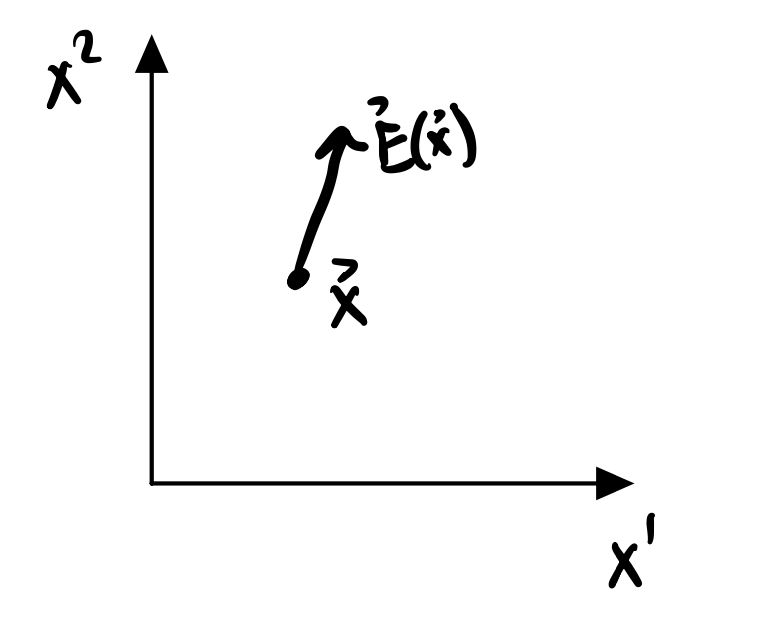
\includegraphics[scale=0.35]{Lectures/Images/lec4-vectorfield.png}
\end{center}

and you can convince yourself that vector fields have the following transformation:
\begin{equation}
    E'_i(\v{x}')dx'^i = E_i(\v{x})dx^i
\end{equation}

\subsection{Gauge Fields}

What we would like to do is generalize this to all Lorentz transformations, where four-vectors $x^\mu = (t, \v{x})$ transform as:
\begin{equation}\label{eq:spacetimecoordLorentztransformation}
    x'^\mu = \Lambda^{\mu}_{\sp\nu}x^\nu.
\end{equation}
The issue now becomes that it is unclear how $\v{E}, \v{B}$ (which are \emph{not} 4-vectors) transform. The main hint is that we may write the electric and magnetic fields in terms of a scalar and vector potential:
\begin{equation}
    \v{E} = -\nabla \phi - \dot{\v{A}}
\end{equation}
\begin{equation}
    \v{B} = \nabla \times\v{A}
\end{equation}
there is a sense in which $\phi, \v{A}$ are more fundamental than $\v{E}, \v{B}$, which we will see later in the lecture.Now, we are back to a problem that we have previously encountered. We have a scalar $\phi$ and a vector $\v{A}$, so it makes sense to package them into a single four-vector, known as the gauge field:
\begin{equation}
    A^\mu = (\frac{\phi}{c}, \v{A})
\end{equation}
The question then becomes whether or not this is a useful definition, and the answer is yes! 

Under Lorentz transformations, we expect:
\begin{equation}
    A_\mu(x')dx'^\mu = A_\nu(x)dx^\nu
\end{equation}
before we move on, it's worth picking apart exactly what this means; if we divide both sides by $dx^\nu$:
\begin{equation}
    A_\mu'(x')\frac{dx'^\mu}{dx^\nu} = A_\nu(x)
\end{equation}

Now, the derivative we can read off from Eq. \eqref{eq:spacetimecoordLorentztransformation}:
\begin{equation}
    \frac{dx'^\mu}{dx^\nu} = \Lambda^{\mu}_{\sp\nu}
\end{equation}
so then:
\begin{equation}
    A_\mu'(x')\Lambda^{\mu}_{\sp\nu}= A_\nu(x)
\end{equation}

\subsection{Field Strength}
Now, we have to check what the implication this is for on the $\v{E}, \v{B}$ - the answer is that we can define the field strength of the gauge field:
\begin{equation}
    F_{\mu\nu} = \p_\mu A_\nu - \p_\nu A_\mu
\end{equation}
where $\p_\mu = \ddpd{}{x^\mu}$. I have a suspicion that $F_{\mu\nu}$ has something to do with $\v{E}, \v{B}$. The first reason is that $F_{\mu\nu}$ is a $4\times 4$ antisymmetric matrix:
\begin{equation}
    F_{\mu\nu} = -F_{\nu\mu}
\end{equation}
which contains 6 independent components, which matches the total number of independent components stored in the $\v{E}, \v{B}$. The other reason is that $F_{\mu\nu}$ is gauge invariant. Last quarter, you noticed that, for an arbitrary scalar function $\chi$, we could transform the scalar/vector potential as:
\begin{equation}
    \phi' = \phi - \p_t \chi, \quad \v{A}' = \v{A} + \nabla \chi
\end{equation}
and under such a transformation $\v{E}, \v{B}$ are invariant. Such transformations are known as gauge transformations, and are labelled by an arbitrary scalar function of spacetime. In order to discuss what happens to $F_{\mu\nu}$ under such transformations, we first act how the gauge field $A_\mu(x)$ transforms under such a transformation:
\begin{equation}
    A_\mu'(x) = A_\mu(x) + \p_\mu \chi
\end{equation}
Let's check this for the 0-th/time component:
\begin{equation}
    A_0' = A_0 + \ddpd{}{x^0}\chi \implies -\frac{\phi'}{c} = -\frac{\phi}{c} + \dpd{}{(ct)}\chi \implies \phi' = \phi - \p_t \chi
\end{equation}
and the story for the spatial components is analogous. With this, let's check how the field strength transforms:
\begin{equation}
    F_{\mu\nu}' = \p_\mu A_\nu' - \p_\nu A_\mu' = \p_\mu(A_\nu + \p_\nu\chi) - \p_\nu(A_\mu + \p_\mu \chi) = F_{\mu\nu} + \p_\mu\p_\nu\chi - \p_\nu\p_\mu\chi = F_{\mu\nu}
\end{equation}
it is invariant! So now we're pretty confident that the components of $F$ will give the components of the $\v{E}/\v{B}$ fields. Let's work them out:
\begin{equation}
    F_{i0} = -F_{0i} = \p_i A_0 - \p_0 A_i = -\frac{1}{c}\p_i \phi - \p_0 A_i = \frac{1}{c}E_i
\end{equation}
\begin{equation}
    F_{12} = -F_{21} = \p_1 A_2 - \p_2 A_1 = \e_{3jk}\p_j A_k = B_3
\end{equation}
(where in the last equality we recall that $B_i = \e_{ijk}\p_j A_k$). Thus for the general component of the B-field:
\begin{equation}
    B_i = \frac{1}{2}\e_{ijk}F_{jk}
\end{equation}
the $\frac{1}{2}$ coming from the fact that when we do the $j, k$ summations we get two nonzero terms. The bottom line of this discussion:
\begin{equation}
    F_{\mu\nu} = \m{0 & -\frac{1}{c}E_1 & -\frac{1}{c}E_2 & -\frac{1}{c}E_3 \\ \frac{1}{c}E_1 & 0 & B_3 & -B_2 \\ \frac{1}{c}E_2 & - B_3& 0 & B_1 \\ \frac{1}{c}E_3 & B_2 & -B_1 & 0}
\end{equation}
why did we do all of this? When we first wrote down the Maxwell equations, we had confusion about how $\v{E}, \v{B}$ transform under Lorentz transformations. Now we have answered it - we can combine $\v{E}, \v{B}$ into $F_{\mu\nu}$ and it is easy to see how this transforms, because we know how $A_\mu$ transforms under Lorentz:
\begin{equation}
    F'^{\mu\nu}(x') = \Lambda^{\mu}_{\sp\lambda}\Lambda^{\nu}_{\sp\rho}F^{\lambda\rho}(x)
\end{equation}
This looks very abstract, but it answers very physical questions. Suppose we have a charged particle, eminating an $\v{E}$-field. I could then get on a bike\footnote{Assuming I was very good at riding a bike and I could go close to the speed of light...} and ask what $\v{E}, \v{B}$-fields I observe - this allows us to answer it.

So far, we have just written down a bunch of definitions we hope would be useful. We had Maxwell's equations, and we wanted to make sure they were invariant under Lorentz transformations. Now, we are in a position to go back to this question, and ask if we can write Maxwell's equations in a way where the Lorentz invariance is manifest.

\subsection{Lorentz Covariant Maxwell Equations}
We require one more definition, that of the dual field strength. We have the field strength:
\begin{equation}
    F_{\mu\nu} = \p_\mu A_\nu - \p_\nu A_\mu
\end{equation}
and then its dual is defined by:
\begin{equation}
    {F^*}^{\alpha\beta} = \tilde{F}^{\alpha\beta} \coloneqq \frac{1}{2}\e^{\alpha\beta\gamma\delta}F_{\gamma\delta}
\end{equation}
where:
\begin{equation}
    \e^{0123} = 1
\end{equation}
and every time two indices are flipped we get a $-1$ sign. The $\frac{1}{2}$ in the definition is there to account for the fact that we get two factors in the summation over $\gamma, \delta$. 

We can explicitly work out the components:
\begin{equation}
    \tilde{F}_{\mu\nu} = \m{0 & B_1 & B_2 & B_3 \\ -B_1 & 0 & \frac{1}{c}E_3 & -\frac{1}{c}E_2 \\ -B_2 & -\frac{1}{c}E_3 & 0 & \frac{1}{c}E_1 \\ -B_3 & \frac{1}{c}E_2 & -\frac{1}{c}E_1 & 0}
\end{equation}
from which we can see that $F, \tilde{F}$ are related via $\v{E} \to c\v{B}, c\v{B} \to -\v{E}$. This is the beginning of a rabbit hole known as electromagnetic duality, and it has lead theorists to believe that there exist magnetic monopoles.

We claim that the dual tensor satisfies:
\begin{equation}
    \p_\mu \tilde{F}^{\mu\nu} = 0
\end{equation}
Let's prove this; fully writing out the dual tensor:
\begin{equation}
    \tilde{F}^{\mu\nu} = \e^{\mu\nu\gamma\delta}(\p_\gamma A_\delta - \p_\delta A_\gamma)
\end{equation}
Now taking the derivative;
\begin{equation}
    \p_\mu \tilde{F}^{\mu\nu} = \e^{\mu\nu\gamma\delta}(\p_\mu\p_\gamma A_\delta - \p_\mu \p_\delta A_\gamma)
\end{equation}
Note that the derivative terms are symmetric under $\mu \leftrightarrow \gamma$ and $\mu \leftrightarrow \delta$, but $\e^{\mu\nu\gamma\delta}$ is antisymmetric under such interchanges; hence the derivative vanishes:
\begin{equation}
    \boxed{\p_\mu \tilde{F}^{\mu\nu} = 0}
\end{equation}
and we call this the \emph{Bianchi identity}. Actually, it is four equations, one for each $\nu = 0, 1, 2, 3$. We can write this identity in terms of electric and magnetic fields:
\begin{equation}
    \nabla \cdot \v{B} = 0
\end{equation}
\begin{equation}
    \nabla \times \v{E} + \dot{\v{B}} = 0
\end{equation}
which we can see are just two of the Maxwell equations - the equations are really Lorentz covariant, because we can write them in terms of $\tilde{F}^{\mu\nu}$, so if they are satisfied in one frame we can easily deduce that they are in a boosted frame.

We then have the other two equations which don't straightforwardsly follow from the Bianchi identity:
\begin{equation}
    \nabla \cdot \v{E} = \frac{\rho}{\e_0}
\end{equation}
\begin{equation}
    \nabla \times \v{B} - \frac{1}{c}\dot{\v{E}} = \mu_0\v{J}
\end{equation}

The charge and current densities satisfy the continuity equation:
\begin{equation}
    \dot{\rho} + \nabla \cdot \v{J} = 0
\end{equation}
at this point, we're Pavlovian dogs who start drooling whenever we see a scalar and a vector together, so we're motivated to define:
\begin{equation}
    J^\mu = (c\rho, \v{J})
\end{equation}
wherein the continuity equation just reads:
\begin{equation}
    \p_\mu J^\mu = 0 
\end{equation}

Under Lorentz transformations:
\begin{equation}
    J'^\mu(x')dx'_\mu = J^\nu(x)dx_\nu
\end{equation}

So let's get back to the remaining two Maxwell equations; you can convince yourself that:
\begin{equation}
    \boxed{\p_\mu F^{\mu\nu} = -\mu_0 J^\nu}
\end{equation}
which is the relativistically covariant form of the Maxwell equations relating the fields to charges/currents.

One thing to point out - when we write this, one thing that is obvious is that if we can write this at all, the current must be conserved. The reason is that if that if I take the derivative $\p_\nu$:
\begin{equation}
    \p_\nu \p_\mu F^{\mu\nu} = -\mu_0 \p_\nu J^\nu
\end{equation}
on the LHS we have a trivial zero (symmetric derivative of an antisymmetric tensor) so:
\begin{equation}
    \p_\nu J^\nu = 0
\end{equation}
the current must be conserved. Said another way, the electromagnetic field can only couple consistently to conserved currents.

A comment - on Tuesday, we discussed the dynamics of free particles. We might ask whether we've solved the problem of charged particles here - the answer is not quite, since throughout we've assumed $\rho, \v{J}$ are smooth and a charged pointlike particle would give rise to a delta-function concentrated charge/current. But we'll see how to deal with this later.

\subsection{Lagrangian Formulation}
We have found the Maxwell equations:
\begin{equation}
    \p_\mu \tilde{F}^{\mu\nu} = 0
\end{equation}
\begin{equation}
    \p_\mu F^{\mu\nu} = -\mu_0 J^\nu
\end{equation}
and we want to know whether we can get these equations from Euler-Lagrange equations that follow from some Lagrangian.

First, we review the situation in point-particle mechanics. Then, we generalize to field theory. Finally, we will specialize to E\& M.

In classical mechanics, we have generalized coordinates $q_i(t)$ for $i = 1, \ldots n$. The action is then:
\begin{equation}
    S = \int dt \mathcal{L}(q_i, \dot{q}_i)
\end{equation}
for $\mathcal{L} = T - U$. The Euler-Lagrange equations are then:
\begin{equation}
    \dod{}{t}\dpd{\LL}{\dot{q}_i} = \dpd{\LL}{q_i}
\end{equation}
and you have solved this, e.g., when $T = \frac{1}{2}\sum_i m_i \dot{q}_i^2$ and $U = U(q_1, \ldots q_n)$. 

We now want to promote these coordinates to fields, $q_i(t) \to \phi_i(t, \v{x})$, and we shall continue with this next lecture.
\section{Lagrangian for EM field}

In relativistic notation, Maxwell's equations are:

\begin{equation}
    \p_\mu \tilde{F}^{\mu\nu} = 0
\end{equation}
\begin{equation}
    \p_\mu F^{\mu\nu} = -\mu_0 J^{\nu}
\end{equation}
where:
\begin{equation}
    F_{\mu\nu} = \p_\mu A_\nu - \p_\nu A_\mu
\end{equation}
\begin{equation}
    \tilde{F}^{\mu\nu} = \frac{1}{2}\e^{\mu\nu\rho\sigma}F_{\rho\sigma}
\end{equation}
we then raised the question: could we derive these equations from a Lagrangian?

\subsection{From particles to fields}
Brief review of classical mechanics of particles - we consider an action:
\begin{equation}
    S = \int dt \mathcal{L}(q_i(t), \dot{q}_i(t))
\end{equation}
Which, extremizing, we obtain the Euler-Lagrange equations:
\begin{equation}
    \dod{}{t}\dpd{\LL}{\dot{q}_i} = \dpd{\LL}{q_i}
\end{equation}
which are equivalent to Newton's second law.

We now generalize, in two steps. First, we generalize the generalized coordinates $q_i(t)$ to a field $\phi$:
\begin{equation}
    q_i(t) \to \phi(x) = \phi(\v{x}, t)
\end{equation}
Comparing to what we had in the case of particle mechanics, instead of the $i$ index we have the position $\v{x}$ - we have a continuous number of degrees of freedom. Field theory is nothing more than classical mechanics of an infinite degrees of freedom.

We can further generalize:
\begin{equation}
    \phi(x) \to \phi_i(x)
\end{equation}
where $i = 1, \ldots n$. This is not to be confused with the index $i$ for the particle label. This is just saying we have $i = 1, \ldots n$ different fields.

In our application, we take $\phi_i \to A_\mu$. The spacetime index $\mu$ plays the role of $i$. $A_\mu$ is a vector field, and in full gory detail:
\begin{equation}
    A_\mu = A_\mu(x^0, x^1, x^2, x^3)
\end{equation}
with $\mu = 0, 1, 2, 3$. Lorentz transformations act on both indices.

Comment: this is similar to the role of spin in quantum mechanics; we had wavefunctions $\phi(\v{x}, t)$ which we obtained by solving the Schrodinger equation. When we solved for the energy levels of the hydrogen atom, we likely ignored the fact that the electron had spin. But in the presence of the magnetic field, there is a term in the Hamiltonian that acts on the spin, so we add an extra index $\alpha$ to $\psi_{\alpha}(\v{x}, t)$ where $\alpha = \uparrow, \downarrow$. $\mu$ plays an analogous role - we have spin-1.

Going back to the action, we can write (restricting to just one field for now):
\begin{equation}
    S = \int d^4x \mathcal{L}(\phi(x), \p_\mu \phi(x)).
\end{equation}
We want to understand what is the analog of the Euler-Lagrange equations? We will follow the same logic in the particle case - we vary the field $\phi$:
\begin{equation}
    \phi(x) \to \phi(x) + \delta\phi
\end{equation}
where the variation $\delta\phi$ is arbitrary and small\footnote{The proof of the fact that Kusatov has free will is that he can choose any variation he likes, here.}. We then ask by how much does $S(\phi)$ change under the variation, to first order in $\delta \phi$:
\begin{equation}
    \begin{split}
        \delta S &= S(\phi + \delta \phi) - S(\phi) 
        \\ &= \int d^4x\left[\LL(\phi + \delta \phi, \p_\mu \phi + \p_\mu \delta \phi) - \LL(\phi, \p_\mu \phi)\right]
        \\ &= \int d^4x\left[\delta \phi \dpd{\LL}{\phi} + \p_\mu \delta\phi\dpd{\LL}{(\p_\mu \phi)}\right]
        \\ &= \int d^4x\left[\delta \phi \dpd{\LL}{\phi} + \p_\mu\left(\delta \phi \dpd{\LL}{(\p_\mu \phi)}\right) - \delta \phi \p_\mu \dpd{\LL}{(\p_\mu \phi)}\right]
    \end{split}
\end{equation}
Now, the middle term is an integral of a total derivative. We can thus write it as (for $\mu = 0$):
\begin{equation}
    \int d^4x \p_0\left[\left(\dpd{\LL}{(\p_0 \phi)}\right)\delta \phi\right] = \left.\int d^3 x \dpd{\LL}{(\p_0 \phi)}\delta\phi \right|_{x^0 = -\infty}^{x^0 = \infty}
\end{equation}
and we can choose the variation $\delta\phi$ to go to zero at the boundary of time. This is analogously true for the spatial $\mu$s. Thus the total derivative term drops out, and the variation in the action becomes:
\begin{equation}
    \delta S = \int d^4 x \delta \phi(x) \left[\dpd{\LL}{\phi} - \p_\mu \dpd{\LL}{(\p_\mu\phi)}\right] = 0
\end{equation}
and if we want this to hold for all variations $\delta \phi(x)$, we thus obtain:
\begin{equation}
    \dpd{\LL}{\phi} = \p_\mu\dpd{\LL}{(\p_\mu \phi)}
\end{equation}
or in the case of multiple fields:
\begin{equation}
    \boxed{\dpd{\LL}{\phi_i} = \p_\mu\dpd{\LL}{(\p_\mu \phi_i)}}
\end{equation}

\subsection{EM field Lagrangian - no sources}
We want:
\begin{equation}
    S = \int d^4x\mathcal{L}(A_\mu(x), \p_\nu A_\mu(x))
\end{equation}
note that the Lagrangian depends on the gauge potential $A_\mu$ as opposed to the electric/magnetic field. We want to get the Maxwell equations out of the Euler-Lagrange equations:
\begin{equation}
    \dpd{\LL}{A_\nu} = \p_\mu \dpd{\LL}{(\p_\mu A_\nu)}
\end{equation}
What $\LL$ should we choose? First, we have the equation/Bianchi identity:
\begin{equation}
    \p_\mu \tilde{F}^{\mu\nu} = 0
\end{equation}
but this equation is a triviality. This is just true by the definition of the (dual) field strength. So we don't want this from the Lagrangian. What we actually want to derive from the Lagrangian is:
\begin{equation}
    \p_\mu F^{\mu\nu} = -\mu_0 J^\nu
\end{equation}
For simplicity, let's start in the case with $J^\nu = 0$. We then want to reproduce:
\begin{equation}
    \p_\mu F^{\mu\nu} = \p_\mu(\p^\nu A^\nu - \p^\nu A^\mu) = 0.
\end{equation}
$\LL$ should satisfy some properties:
\begin{itemize}
    \item  $\LL$ should be Lorentz invariant - this is because $S$ should be Lorentz invariant, and $d^4x$ is Lorentz invariant.
    \item $\LL$ should be gauge invariant - the Maxwell equation and physics we get out of it should be gauge invariant.
    \item The Euler-Lagrange equation is linear in $A_\mu$ - thus $\LL$ should be quadratic in $A_\mu$.
\end{itemize}

Given these conditions, we have only three objects we could conceivably write\footnote{If you can think of another, please tell Kusatov, and he will immediately run to write a paper on it without you.}:
\begin{itemize}
    \item $-F_{\mu\nu}F^{\mu\nu}$
    \item $-F_{\mu\nu}\tilde{F}^{\mu\nu}$
    \item $-\tilde{F}_{\mu\nu}\tilde{F}^{\mu\nu}$
\end{itemize}
Note that $-\tilde{F}_{\mu\nu}\tilde{F}^{\mu\nu}$ is proportional to $-F_{\mu\nu}F^{\mu\nu}$ and so is not a unique possibility, and $-F_{\mu\nu}\tilde{F}^{\mu\nu}$ is a total derivative and so does not contribute to the physics. We thus have one possibility remaining:
\begin{equation}
    \LL_{\text{EM}} = -\frac{1}{4\mu_0}F_{\mu\nu}F^{\mu\nu}
\end{equation}
The proportionality constant we put there for later convenience, but this is not important for the purposes of the Euler-Lagrange equation. In the next problem set, you can verify that the E-L equation yields precisely $\p_{\mu}F^{\mu\nu} = 0$. This must work - if it did not, there would be no Lagrangian that could possibly works, and we just wasted 2 weeks of your time. Writing $\LL$ in terms of the electromagnetic fields, we have:
\begin{equation}
    \LL_{\text{EM}} = \frac{1}{2\mu_0}\left(\frac{1}{2}\abs{\v{E}}^2 - \abs{\v{B}}^2\right)
\end{equation}
wherein we can immediately see that the Euler-Lagrange procedure would be doomed to fail if we had used $\v{E}, \v{B}$ as the fundamental degrees of freedom.

\subsection{EM field Lagrangian - with sources}
If we want to reproduce the case with sources:
\begin{equation}
    \p_{\mu}F^{\mu\nu} = -\mu_0 J^\nu
\end{equation}
we can simply add the term:
\begin{equation}
    \LL = -\frac{1}{4\mu_0}F^{\mu\nu}F_{\mu\nu} + A_\mu J^\mu.
\end{equation}

But actually there is a problem here. This Lagrangian is \emph{not} gauge invariant. If we perform the gauge transformation:
\begin{equation}
    A_\mu \to A_\mu - \p_\mu \chi
\end{equation}
Then the Lagrangian picks up a new term:
\begin{equation}
    \delta \LL = -J^\mu \p_\mu \chi
\end{equation}

Is this a problem? Actually, no. What we \emph{really} want is not that $\LL$ is gauge invariant, but that the action $S$ is gauge invariant. In other words, does $\delta S$ from making the gauge transformation vanish?
\begin{equation}
    \delta S = \int d^4x \delta \LL = -\int d^4x J^\mu \p_\mu \chi = -\int d^4x \p_\mu[J^\mu \chi]
\end{equation}
In the last line, we wrote things as a total derivative; this is valid as:
\begin{equation}
    \p_\mu [J^\mu \chi] = (\p_\mu J^\mu)\chi + J^\mu (\p_\mu \chi) = J^\mu (\p_\mu \chi)
\end{equation}
as $\p_\mu J^\mu = 0$ (continuity equation/current conservation). Going back to $\delta S$, we can have some discussion about the integral of the total derivative. As we discussed earlier in lecture, this only receives contributions from the boundaries of spacetime. So, the action is invariant under gauge transformations that go to zero rapidly to zero at the boundaries of spacetime. But if we include $\chi$s that do \emph{not} go to zero, we get physically important boundary terms - they are relevant to charge conservation. But in this course we do not consider such cases.

Another point to make - the discussion heavily relies on the fact that the current $J^\mu$ is conserved. If we want the action to be invariant under gauge transformations, we can only couple the electromagnetic field to conserved currents.

\subsection{The stress-energy tensor}
Now, we can ask what this Lagrangian is good for - of course, we already have the Euler-Lagrange equation; another answer is we can get the stress-energy tensor for the EM field. Why is this physically important? You are already viscerally aware of the fact that particles have energy and momenta. But you also expect that the electromagnetic field also has this property. What is the analogue of the energy/momentum of a bowling ball for an EM wave?

To review, let's just remind ourselves of how things work for particles. There, we have momenta:
\begin{equation}
    p_i = \dpd{\LL}{\dot{q}_i}
\end{equation}
and the Hamiltonian:
\begin{equation}
    \mathcal{H} = p_i \dot{q}^i - \LL
\end{equation}
where if the Lagrangian does not depend on time, $\mathcal{H} = E$ is the conserved energy. We want to generalize this discussion to fields. We have the action:
\begin{equation}
    S = \int d^4x\LL(\phi, \p_\mu \phi)
\end{equation}
and if there is no explicit dependence on $x^\mu$, then we expect that the action is invariant under $x^\mu \to x^\mu + a^\mu$, and so we expect $p_\mu$ to be conserved.

Let us recall the example of electric charge. We have a conserved current:
\begin{equation}
    \p_\mu J^\mu = 0.
\end{equation}
Why do we care? If we define a charge:
\begin{equation}
    Q = \int d^3x J^0(\v{x}, t)
\end{equation}
where $\dot{Q} = 0$ as:
\begin{equation}
    \dot{Q} = (\text{Const.})\int d^3x\p_0 J^0 = (\text{Const.})\int d^3 x \nabla \cdot \v{J} = 0
\end{equation}
where the last equality follows from current conservation if we integrate over all space (if we integrate over a finite region, we keep track of the charge that flows in/out of a region). Note that $Q$ here is a scalar quantity. This is true because $J^\mu$ is a a Lorentz vector.

What about $p^\mu$? What is the conserved current in this case> Here we expect a tensor $T^{\mu\nu}$ which satisfies $p_\mu T^{\mu\nu} = 0$. Why is this the case?
\begin{equation}
    p^\nu = \int d^3x T^{0\nu}
\end{equation}
so:
\begin{equation}
    \dot{p}^\nu = (\text{Const.})\int d^3x \p_0 T^{0\nu} = (\text{Const.})\int d^3x \p_i T^{i\nu} = 0
\end{equation}
if we integrate over all space. We want a tensor so that the conserved quantity $p^\nu$ we get out of it is a Lorentz vector.

We define the stress-energy tensor as:
\begin{equation}
    T^{\mu\nu} = \dpd{\LL}{(\p_\mu \phi^i)}\p^\nu \phi^i - \eta^{\mu\nu}\LL.
\end{equation}
Let us verify that the conservation equation:
\begin{equation}
    \p_\mu T^{\mu\nu} = 0
\end{equation}
is satisfied.
\begin{equation}
    \begin{split}
        \p_\mu T^{\mu\nu} &= \p_\mu\left(\ddpd{\LL}{(\p_\mu \phi^i)}\p^\nu \phi^i\right) - \eta^{\mu\nu}\p_\mu \LL
        \\ &= \p_\mu\left(\ddpd{\LL}{(\p_\mu \phi^i)}\right) \p^\nu \phi^i + \dpd{\LL}{(\p_\mu \phi^i)}\p_\mu \p^\nu \phi_i - \p^\nu \LL(\phi^i, \p_\mu \phi^i)
        \\ &= \ddpd{\LL}{\phi^i} \p^\nu \phi^i + \dpd{\LL}{(\p_\mu \phi^i)}\p_\mu \p^\nu \phi_i - \p^\nu \LL(\phi^i, \p_\mu \phi^i)
        \\ &= 0
    \end{split}
\end{equation}
where in the third equality we use the Euler-Lagrange equation, and in the last equality we can recognize the terms to cancel out using the chain rule to evaluate the derivative of the Lagrangian.

Next time, we study $T^{\mu\nu}$ for an EM field.
\section{Stress Tensor, Angular Momentum, Scale Invariance of EM field}

Last time, we found the Lagrangian and thus action for a field:
\begin{equation}
    S = \int d^4x \mathcal{L}(\phi^i, \p_\mu \phi)
\end{equation}
we then defined the stress tensor:
\begin{equation}
    \tilde{T}^{\mu\nu} = \frac{\delta \LL}{\delta \p_\mu \phi_i}\p^\nu \phi^i - \eta^{\mu\nu}
\end{equation}
which is a conserved quantity (from the Euler-Lagrange equations):
\begin{equation}
    \p_\mu \tilde{T}^{\mu\nu} = 0
\end{equation}
This implies that the momenta:
\begin{equation}
    P^\nu = \int d^3x \tilde{T}^{0\nu}
\end{equation}
are conserved charges.

\subsection{Specific case of the EM stress tensor}

Today, we see what this looks like in the case of the EM field. We have the Maxwell Lagrangian:
\begin{equation}
    \LL_{\text{EM}} = -\frac{1}{4\mu_0}F^{\mu\nu}F_{\mu\nu}
\end{equation} 
with:
\begin{equation}
    F_{\mu\nu} = \p_\mu A_\nu - \p_\nu A_\mu
\end{equation}
\begin{equation}
    A_\mu \leftrightarrow \phi_i
\end{equation}
So the stress-tensor looks like:
\begin{equation}
    \tilde{T}^{\mu\nu} = \frac{\delta \LL}{\delta \p_\mu A^\lambda}\p^\nu A_\lambda - \eta^{\mu\nu}\LL_{\text{EM}}
\end{equation}
from our general argument last class, it is automatically true that:
\begin{equation}
    \p_\mu \tilde{T}^{\mu\nu} = 0
\end{equation}
Computing the stress tensor from the Lagrangian:
\begin{equation}
    \tilde{T}^{\mu\nu} = \frac{1}{\mu_0}F^{\mu\lambda}\p^\nu A_\lambda - \eta^{\mu\nu}\LL_{\text{EM}}
\end{equation}

\subsection{Issues with the Definition \& Resolution}
There are two problems:
\begin{itemize}
    \item $\tilde{T}^{\mu\nu}$ is not gauge invariant.
    \item $\tilde{T}^{\mu\nu} \neq \tilde{T}^{\nu\mu}$.
\end{itemize}
Why is the second one a problem? Well, there \emph{should} exist a symmetric $T^{\mu\nu}$. 

Suppose we put electromagnetism on a curved spacetime with arbitrary metric $g^{\mu\nu}$. In that case, our Maxwell Lagrangian takes the form:
\begin{equation}
    \LL_{\text{EM}} = -\frac{1}{4\mu_0}g^{\mu\alpha}g^{\nu\beta}F_{\mu\nu}F_{\alpha\beta}\sqrt{-g}
\end{equation}
where $g = \det g_{\mu\nu}$. I can then define the stress tensor in an alternative fashion:
\begin{equation}
    T^{\mu\nu} = -\frac{2}{\sqrt{-g}}\frac{\delta \LL_{\text{EM}}}{\delta g_{\mu\nu}}
\end{equation}
The claim is that this stress tensor also satisfies the conservation equation:
\begin{equation}
    \p_\mu T^{\mu\nu} = 0
\end{equation}
if you're familiar with GR, you wouldn't be surprised by this fact, because the stress tensor is how the metric couples to matter.

Why all of this sidetracking? This new stress tensor is gauge invariant (we get it by taking the functional derivative of a gauge-invariant $\LL$ with respect to a gauge invariant metric) and also is manifestly symmetric (the metric is symmetric).

Let's now try to compute $T^{\mu\nu}$ using this new definition and then see how it differs with our previous result:
\begin{equation}
    T_{\mu\nu} = \frac{1}{\mu_0}\left(F_{\mu}^{\sp\alpha}F_{\nu\alpha} - \frac{1}{4}\eta_{\mu\nu}F_{\alpha\beta}F^{\alpha\beta}\right)
\end{equation}

A short calculation shows that the difference between $T^{\mu\nu}, \tilde{T}^{\mu\nu}$ is:
\begin{equation}
    T^{\mu\nu}_{\Delta} \cong F^{\mu\lambda}\p_\lambda A^\nu
\end{equation}
The question then becomes - is $T^{\mu\nu}_{\Delta}$ something that has a physical consequence?
\begin{itemize}
    \item It's clear that $\p_\mu T^{\mu\nu}_{\Delta} = 0$ as:
    \begin{equation}
        \p_\mu T^{\mu\nu}_{\Delta} = \p_\mu (T^{\mu\nu} - \tilde{T}^{\mu\nu}) = \p_\mu T^{\mu\nu} - \p_\mu \tilde{T}^{\mu\nu} = 0 - 0 = 0
    \end{equation}
    but we can check it explicitly:
    \begin{equation}
        \p_\mu T^{\mu\nu}_{\Delta} = (\p_\mu F^{\mu\nu})\p_\lambda A^\nu + F^{\mu\nu}\p_\mu \p_\lambda A^\nu = 0 + 0 = 0
    \end{equation}
    The first term vanishes via the source-free Maxwell equation, and the second term vanishes as we multiply a symmetric $\p_\mu \p_\lambda A^\nu $ by an antisymmetric $F^{\mu\nu}$.

    \item $\int d^3x T^{0\nu}_{\Delta} = 0$ as it is an integral of a total derivative:
    \begin{equation}
        T^{0\nu}_\Delta = \p_\lambda(F^{0\lambda}A^\nu)
    \end{equation}
    The $\lambda = 0$ term is absent in this sum (as $F^{00} = 0$) and the other terms are spatial derivatives - i.e. a total derivative which vanishes (assuming no boundary terms) when integrated over all space.
\end{itemize}
The upshot is that the two definitions are physically equivalent.

\subsection{Intepreting the Stress-Energy Tensor}
What interpretation does the stress-energy tensor (and its conservation) have? The $00$ component can be interpreted as the energy density:
\begin{equation}
    T_{00} = \frac{1}{2\mu_0}\left(\frac{1}{c^2}\abs{\v{E}}^2 + \abs{\v{B}}^2\right) = \frac{\e_0}{2}\abs{\v{E}}^2 + \frac{1}{2\mu_0}\abs{\v{B}}^2
\end{equation}
The $0i$ component looks like:
\begin{equation}
    T_{0i} = T_{i0} = \frac{1}{\mu_0 c}\left(\v{E} \times \v{B}\right)_i
\end{equation}
where $-\frac{T_{0i}}{c}$ has interpretation as the momentum density. It has another role; $-cT_{0i}$ is the Poynting vector, which is the energy flux of the EM field.

Recall:
\begin{equation}
    P^0 = \int d^3x T^{00} \implies \dot{P}^0 = \int d^3x \dot{T}^{00}
\end{equation}
and the conservation of the stress-energy tensor tells us:
\begin{equation}
    \p_\mu T^{\mu0} = 0 \implies \p_0 T^{00} + \p_i T^{i0} = 0
\end{equation}
so $T^{i0}$ (from conservation) tells us about the energy flux.

\subsection{Rotational Invariance}
The fact that Maxwell theory is rotationally invariant implies by Noether's theorem that there is a conserved angular momentum. Just as there was energy/momentum conservation arising from time/space translation invariance, there must be an analogous story here. One way to think about this is the following. Lorentz symmetry implies that there are conserved charges for both boosts and rotations. In 3+1D, there are 3 boosts and 3 rotations, so we should have 6 conserved charges arising from Lorentz symmetry. We could then ask how these charges transform under Lorentz transformations. $P^\mu$ transformed as a vector (1 energy + 3 momentum components) under Lorentz transformations. We might at first be puzzled by the 6 components we see here, but this is analogous to the 3 + 3 components of the $\v{E}/\v{B}$ field which we packaged into a $4\times 4$ antisymmetric tensor - we do the same here, and expect a tensor $M_{\mu\nu}$ where $M_{0i}$ correspond to boosts and $M_{ij}$ correspond to rotations. We expect that there are conserved charges $L_i$ that satisfy:
\begin{equation}
    M_{ij} = \e_{ijk}L_k
\end{equation}

All of this is to say - if we are interested in constructing the angular momentum charge carried by some electromagnetic field, we have to understand how to get these from Lorentz symmetry.

\begin{itemize}
    \item The electric charge $Q$ corresponds to a conserved current $J^\mu$ (satisfying $\p_\mu J^\mu = 0$).

    \item The energy/momentum $P^\mu$ correspond to a conserved stress-energy tensor $T^{\mu\nu}$ (a current satisfying $\p_\mu T^{\mu\nu} = 0$).
    
    \item So the angular momentum + the charges associated to boosts $M^{\nu\lambda}$ correspond to a conserved 3-index tensor $M^{\mu\nu\lambda}$ (a current satisfying $\p_\mu M^{\mu\nu\lambda}$).
\end{itemize}
A hint from classical mechanics is that $\v{L} = \v{r} \times \v{p}$. So a good guess would be to take the stress-energy tensor and multiply it by a factor of position to get the $M^{\mu\nu\lambda}$. Indeed:
\begin{equation}
    M^{\mu\nu\lambda} = T^{\mu\nu}x^\lambda - T^{\mu\lambda}x^\nu
\end{equation}
Indeed this satisfies:
\begin{equation}
    \p_\mu F^{\mu\nu\lambda} = 0
\end{equation}
to check this, note the relation:
\begin{equation}
    \p_\mu x^\lambda = \ddpd{x^\lambda}{x^\mu} = \eta^{\lambda}_{\sp\mu}.
\end{equation}
Now calculating:
\begin{equation}
    \begin{split}
        \p_\mu M^{\mu\nu\lambda} &= (\p_\mu T^{\mu\nu}) x^\lambda + T^{\mu\nu}(\p_\mu x^\lambda) - (\p_\mu T^{\mu\lambda})x^\nu - T^{\mu\lambda}(\p_\mu x^\nu)
        \\ &= 0 + T^{\mu\nu}\eta^{\lambda}_{\sp\mu} - 0 - T^{\mu\lambda}\eta^{\nu}_{\sp\mu}
        \\ &= T^{\lambda\nu} - T^{\nu\lambda}
        \\ &= 0
    \end{split}
\end{equation}
where the last equality follows from the fact that $T^{\mu\nu}$ is symmetric. Hence the current is indeed conserved. Using this, we can write down a formula for the angular momentum for an EM field.

\begin{equation}
    \v{L} = \e_0 \int d^3x \v{x} \times (\v{E} \times \v{B})
\end{equation}

This makes perfect sense. In fact, we already knew what the momentum density was, and we knew the angular momentum was $\v{L} = \v{r} \times \v{p}$.

\subsection{Scale Invariance}
% Another, slightly more subtle symmetry of the EM field is that it is invariant under scale transformations. 
We observe that $T^{\mu\nu}$ is traceless:
\begin{equation}
    T_{\mu}^{\sp\mu} = T_{\mu\nu}\eta^{\mu\nu} = 0
\end{equation}
what is the significance of this fact? We can write down a conserved current:
\begin{equation}
    J^\mu_{D} = T^{\mu\nu}x_\nu
\end{equation}
and the nice part about this definition is that:
\begin{equation}
    \p_\mu J^{\mu}_D = 0
\end{equation}
Which if we explicitly work out:
\begin{equation}
    \p_\mu (T^{\mu\nu}x_\nu) = (\p_\mu T^{\mu\nu})x_\nu + T^{\mu\nu}(\p_\mu x_\nu) = 0 + T^{\mu\nu}\eta_{\mu\nu} = 0
\end{equation}
the conservation follows from the traceless condition.

What symmetry of the action gives rise to this conserved current?
\begin{equation}
    S_{\text{EM}} = -\frac{1}{4\mu_0}\int d^4x F^{\mu\nu}F_{\mu\nu}
\end{equation}
As the title of this section gives away, the action is invariant under the rescaling:
\begin{equation}
    x' = \alpha x, \quad A'_\mu(x') = \frac{1}{\alpha}A_\mu(x)
\end{equation}'
Let's work this out:
\begin{equation}
    S'_{\text{EM}} = -\frac{1}{4\mu_0}\int d^4x' F_{\mu\nu}'(x')F'^{\mu\nu}(x')
\end{equation}
where:
\begin{equation}
    F_{\mu\nu}'(x') = \ddpd{A'_\nu}{x'^\mu} - \ddpd{A'_\mu}{x'^\nu} = \frac{1}{\alpha^2}F_{\mu\nu}(x)
\end{equation}
So then:
\begin{equation}
    F'^2 = \frac{1}{\alpha^4}F^2
\end{equation}
and the measure also gets rescaled:
\begin{equation}
    d^4x' = \alpha^4 d^4x
\end{equation}
So the $\alpha^4$s cancel and so:
\begin{equation}
    S'_{\text{EM}} = S_{\text{EM}}
\end{equation}
for any $\alpha$. Our conserved current associated to this symmetry (dilations) is $J^\mu_D$.

Three comments about this story:
\begin{itemize}
    \item Remarkably, the scale invariance works out perfectly in 4-dimensions - we use the dimensionality when rescaling the measure - but things do not work the same in lower/higher dimensions.
    \item We can view the entire scale invariance story as follows. We can assign scaling dimensions to quantities. If $\theta \to \frac{1}{\alpha^n}\theta$, then $\theta$ is said to have scaling dimension $n$. Since $x \to \alpha x$, $[x] = -1$, and analogously $[A_\mu] = +1, [P^\mu] = +1$ and so on. The action has $[S] = 0$, which means it is invariant - this is because $[d^4x] = -4$ and $[F_{\mu\nu}] = [\p A] = 1 + 1 = 2$ (from the derivative and from $A$). So $[S] = 0$ comes from $[S] = [F^2] + [d^4x] = 2 \cdot 2 - 4 = 0$.
    \item When we couple to charged matter, formally we still have the symmetry. How to see this? We have in this case that:
    \begin{equation}
        \delta \LL = A_\mu J^\mu
    \end{equation}
    if we want $[\delta \LL] = +4$ so as to retain the scale invariance (cancel out the $-4$ from the measure), then since $[A_\mu] = +1$, we want $[J^\mu] = +3$. Superficially, it looks like we land on our feet because:
    \begin{equation}
        Q =  \int d^3x J^0
    \end{equation}
    Since charge is not measured in meters/is invariant under rescaling, and then $[Q] = 0$ and $[d^3x] = -3$ so $[J] = +3$. But actually, this is a little bit too naive, and we will things break when we couple charged particles to the EM field. If we recall the dispersion:
    \begin{equation}
        E^2 = (pc)^2 + (mc^2)^2
    \end{equation}
    the dispersion is scale-invariant if $m = 0$ but otherwise is not scale invariant (as the mass gets rescaled) - dilations are not a symmetry.
\end{itemize}

Our next topic (next week) is discussing how plane waves look like in relativistic variables - we will see that they look quite elegant.
\section{Plane Waves, Charged Particles Coupled to EM Fields}

\subsection{Plane Waves}
You've already seen plane waves before, but here we discuss it in the Lorentz covariant formalism.

Recall Maxwell's equations:
\begin{equation}
    \p_\mu F^{\mu\nu} = 0
\end{equation}
\begin{equation}
    F_{\mu\nu} = \p_\mu A_\nu - \p_\nu A_\mu
\end{equation}
with the gauge potential:
\begin{equation}
    A_\mu = \left(-\frac{\phi}{c}, A_1, A_2, A_3\right)
\end{equation}
In the Lorenz gauge, we have:
\begin{equation}
    \frac{1}{c^2}\dot{\phi}^2 + \nabla \cdot \v{A} = 0
\end{equation}
in our four-vector notation this takes the elegant and manifestly Lorentz\footnote{Kutasov: This looks like a private joke by God...} covariant form:
\begin{equation}
    \p_\mu A^\mu = 0
\end{equation}
The reason why Wald likes the Lorentz gauge is that in this gauge, the four components of $A^\mu$ satisfy the wave equation:
\begin{equation}
    \square A^\mu = 0
\end{equation}
where:
\begin{equation}
    \square = \eta^{\mu\lambda}\p_\nu \p_\lambda = \p_\nu\p^\nu 
\end{equation}

In our new formalism, we can write a monochromatic wave as:
\begin{equation}
    A_\mu = \xi_\mu e^{ik_\nu x^\nu}
\end{equation}
With $\xi_\mu$ the polarization vector. The wave equation then says that:
\begin{equation}
    k^\mu k_\mu = 0
\end{equation}
and hence that:
\begin{equation}\label{eq:waveeqcondition}
    k_0^2 = \abs{\v{k}}^2
\end{equation}
The frequency of the wave by definition is:
\begin{equation}
    \omega = ck_0
\end{equation}
So Eq. \eqref{eq:waveeqcondition} is nothing more than a statement of the wave dispersion:
\begin{equation}
    \omega = c\abs{\v{k}}
\end{equation}

\subsection{Polarizations}
What do we know about $\xi_\mu$? It consists of 4 numbers... but we do not expect these to be independent, given that electromagnetic waves have 2 polarizations. Further, we notice that we have not yet imposed the Lorentz gauge to see how they could become constrained. If we do, we find:
\begin{equation}
    \xi_\mu k^\mu = 0
\end{equation}
This condition brings the 4 independent numbers down to 3. We still aren't done yet. The thing we forgot is slightly subtle. We recall that gauge symmetry is the condition that the transformation:
\begin{equation}
    A_\mu \to A_\mu + \p_\mu \chi
\end{equation}
leaves the physics invariant. When we impose the Lorentz gauge, we have fixed the arbitrariness... or have we? Actually, it turns out the Lorentz gauge does not completely fix the gauge freedom. Lorentz gauge says:
\begin{equation}
    \p_\mu A^\mu = 0
\end{equation}
and if we want gauge invariance:
\begin{equation}
    \p_\mu (A^\mu + \p^\mu \chi) = 0
\end{equation}
in other words, if $\xi$ satisfies the wave equation:
\begin{equation}
    \p_\mu \p^\mu \chi = \square \chi = 0
\end{equation}
then we may add $\p_\mu \chi$ to $A_\mu$ - this tells us that we have residual gauge invariance. This is a bit interesting - precisely when the $A^\mu$ is on shell, i.e. when it satisfies the Maxwell equations, the residual gauge freedom kicks in.

If we have $A_\mu = \xi_\mu e^{ik_\nu x^\nu}$ with $k_\mu k^\mu = 0$, then we can add to it the four-derivative ($\p^\mu$) of:
\begin{equation}
    \chi = \chi_0 e^{ik_\nu x^\nu}
\end{equation}
This tells us that we can shift:
\begin{equation}
    \xi_\mu^{(k)} \to \xi_\mu^{(k)} + k_\mu \chi_0^{(k)}
\end{equation}
where we have added the $(k)$ label to denote that it is the polarization corresponding to a particular wavevector.

In summary: plane waves are described by Gauge fields of the form:
\begin{equation}
    A_\mu = \xi_\mu^{(k)}e^{ik_\nu x^\nu}
\end{equation}
where we have the three conditions:
\begin{equation}
    k^2 = k_\mu k^\mu = 0
\end{equation}
\begin{equation}
    k_\mu \xi^{(k)\mu} = 0
\end{equation}
\begin{equation}
    \xi_\mu^{(k)} \sim \xi_\mu^{(k)} + k_\mu \e^{(k)}
\end{equation}
We can now ask how many independent components of $\xi_\mu$ we have. Suppose we have:
\begin{equation}
    k_\mu = (k, 0, 0, k)
\end{equation}
i.e. a wave propagating in the $z$-direction. Let's check the three conditions. $k^2 = 0$ is clearly satisfied. The second condition is:
\begin{equation}
    k_0\xi^0 + k_3 \xi^3 = 0 \implies \xi^0 + \xi^3 = 0 \implies \xi^0 = -\xi^3
\end{equation}
The last condition is:
\begin{equation}
    \xi_0 \sim \xi_0 + k_0 \e = \xi_0 + k\e
\end{equation}
\begin{equation}
    \xi_3 \sim \xi_3 + k_3 \e = \xi_3 + k\e
\end{equation}
So together:
\begin{equation}
    \xi_0 = \xi_3 = 0
\end{equation}
and hence we have the remaining two independent polarizations $\xi = (0, 1, 0, 0)$ and $\xi = (0, 0, 1, 0)$.

\subsection{Lagrangian of Charged Particle Coupled to EM Field - Consistency conditions}
Thus far, we have looked at the action for a free relativistic particle, as well as for free EM fields. Now, we want to study the Lagrangian for a charged particle coupled to an EM field.

Recall the Lagrangian for a free particle:
\begin{equation}
    S_0 = -mc\int d\lambda \sqrt{-\dot{x}_\mu \dot{x}^\mu}
\end{equation}
or in the gauge $t(\lambda) = \lambda$:
\begin{equation}
    S_0 = -mc^2 \int dt\sqrt{1-\frac{\v{v}^2}{c^2}}
\end{equation}

Now, we ask what about charged particles? We write down a natural extension\footnote{But be wary, things that are natural are not automatically correct...}:
\begin{equation}
    \delta S = \alpha\int d\lambda \dot{x}^\mu A_\mu(x)
\end{equation}
We will find that this is reparametrization invariant, gauge invariant, it is manifestly Lorentz invariant (the $\mu$ indices are contracted), and has other properties we require. $\alpha$ appearing in the above is a constant we will determine.

Recall reparameterization invariance:
\begin{equation}
    \int d\lambda \frac{dx^\mu}{d\lambda} \stackrel{\lambda\to f(\lambda)}{=} \int df(\lambda)\frac{dx^\mu}{df(\lambda)}
\end{equation}
where if $x^\mu = x^\mu(f(\lambda))$ then:
\begin{equation}
    \frac{dx^\mu}{d\lambda} = \frac{dx^\mu}{df(\lambda)}\frac{df}{d\lambda}
\end{equation}
This is satisfied by our proposed $\delta S$.

Now, let's think about Gauge invariance; under transformations:
\begin{equation}
    A_\mu \to A_\mu - \p_\mu \chi
\end{equation}
The Lagrangian does \emph{not} look invariant under this. But we recall back to our discussion last week - it is not the Lagrangian that we require to be gauge invariant, but rather the action. Under the gauge transformation, we have (up to some constants that we ignore):
\begin{equation}
    \delta S \to \delta S + (\text{const.})\int d\lambda \dot{x}^\mu \p_\mu \chi
\end{equation}
Looking at this newly generated term
\begin{equation}
    \int_{\lambda_1}^{\lambda_2} d\lambda \dot{x}^\mu \p_\mu \chi \stackrel{\text{chain rule}}{=} \int_{\lambda_1}^{\lambda_2} d\lambda \dod{}{\lambda}\chi(x^\mu(\lambda)) = \left.\chi(x^\mu(\lambda))\right|_{\lambda_1}^{\lambda_2}
\end{equation}
So, the variation only depends on the values of $\chi$ at the boundaries of spacetime - it is thus independent of the local form of $\chi(x^\mu)$. Hence, we conclude that this new term we add to the action is indeed gauge invariant.

\subsection{Fixing the coefficient}
Now, we ask what is the constant $\alpha$? Let us compare it to:
\begin{equation}
    \int d^4 x A_\mu(x)J^\mu(x)
\end{equation}
where the multiplicative constant was constrained by what we wanted on the RHS of the Maxwell equations. Writing the full action (free part + interacting part):
\begin{equation}
    S = \int d\lambda(-mc\sqrt{-\dot{x}_\mu \dot{x}^\mu} + \alpha\dot{x}^\mu A_\mu(x))
\end{equation}
Taking $\lambda = t$:
\begin{equation}
    S = \int dt\left[-mc^2\sqrt{1-\frac{\dot{\v{x}}^2}{c^2}} - \alpha \phi + \alpha \dot{\v{x}}\cdot \v{A}\right]
\end{equation}
Just from this form, it looks like we should make $\alpha = q$. Why? The first term at low velocity looks like the mass energy + low-velocity kinetic energy of the particle, and the terms involving the gauge potentials are just the energy from the interaction of the electric field and the charge of the particle as you saw last quarter.

But let us see this another way. We can calculate the momentum, using the Lagrangian:
\begin{equation}
    p^i = \frac{\delta \LL}{\delta \dot{x}_i} = \frac{m\dot{x}^i}{\sqrt{1 - \frac{\v{v}^2}{c^2}}} + \alpha A^i
\end{equation}
Now, if I go look into your notes for your quantum mechanics class (taking the $\abs{\v{v}} \ll c$ limit) we find $\alpha = q$.

\subsection{Lorentz Force Law}
From the definitions, you can check (and perhaps will soon, on a pset) that the EL equations take the following form:
\begin{equation}
    \dod{\v{p}}{t} = q(\v{E} + \v{v} \times \v{B})
\end{equation}
where:
\begin{equation}
    \v{p} = m\gamma\v{v}
\end{equation}
\begin{equation}
    \v{E} = -\nabla \phi - \dot{\v{A}}
\end{equation}
\begin{equation}
    \v{B} = \nabla \times \v{A}
\end{equation}

A couple comments; first, since our Lagrangian is Lorentz invariant, the Lorentz force law that we get out of it must be Lorentz invariant. It doesn't look manifestly so, but we can write it in this way. First, we can define the proper time $\tau$ via:
\begin{equation}
    c^2 d\tau^2 = -dx^\mu dx_\mu
\end{equation}
This definition is interesting because we can define:
\begin{equation}
    u^\mu = \frac{dx^\mu}{\tau}
\end{equation}
for which:
\begin{equation}
    u^\mu u_\mu = -c^2
\end{equation}
is an invariant. We can then show:
\begin{equation}
    \frac{du^\mu}{d\tau} = -\frac{q}{\gamma m}F^{\mu\nu}u_\nu
\end{equation}
which is a Lorentz covariant form of the Lorentz force law.

\subsection{Charge Density and Current}
Another comment; we already had the coupling:
\begin{equation}\label{eq:AJ}
    \int d^4x A_\mu(x)J^\mu(x)
\end{equation}
and writing down a reasonable choice for $J^\mu$ for a point particle we could have derived:
\begin{equation}
    q\int d\lambda A_\mu(x)\dot{x}^\mu
\end{equation}
but having derived it independently, we can go the opposite direction, and derive what $J^\mu$ for a point particle is from this expression. You can convince yourself that:
\begin{equation}
    \rho(t, \v{x}) = q\delta(\v{x} - \v{x}(t))
\end{equation}
\begin{equation}
    \v{J}(t, \v{x}) = q\dod{\v{x}}{t}\delta(\v{x} -\v{x}(t))
\end{equation}
where a delta function of vectors is defined as:
\begin{equation}
    \delta(\v{x} - \v{x}(t)) = \delta(x - x(t))\delta(y - y(t))\delta(z - z(t))
\end{equation}
Therein:
\begin{equation}
    \int_V d^3x\rho(\v{x}, t) = \begin{cases}
        q & \v{x}(t) \in V
        \\ 0 & \text{otherwise}
    \end{cases}
\end{equation}
as it should. $\v{J}$ is the quantity that keeps track of what happens when the particle goes inside the volume. You can check that this expression correctly satisfies the continuity equation:
\begin{equation}
    \dot{\rho} + \nabla \cdot \v{J} = 0
\end{equation}
You can also check that if you take the $J^\mu$ and substitute it into Eq. \eqref{eq:AJ}, the integral localizes onto the worldline of the particle. 

\subsection{Charged Particle Motion in Constant Electric Field}
We first study the case of $\v{B} = 0, \v{E} = E\xhat$. Now, we want to find the trajectory $\v{x}(t)$ of a particle of charge $q$ in such an $\v{E}$-field. Take $\v{x}(t=0) = 0$ and $\dot{\v{x}}(t=0) = 0$. It is clear that $y(t) = z(t) = 0$ for all $t$; the motion is along the $x$ axis. Now, we have the equation of motion:
\begin{equation}
    \dod{}{t}(\gamma v) = \frac{q}{m}E
\end{equation}
where $\gamma = \frac{1}{\sqrt{1-\frac{v^2}{c^2}}}$. $\gamma v$ is linear in time, so:
\begin{equation}
    \gamma v = \frac{q}{m}Et 
\end{equation}
where there is no $t = 0$ constant at the velocity is 0 at $t=0$. We can now solve for $v$ from the above:
\begin{equation}
    v(t) = \frac{\frac{qE}{m}t}{\sqrt{1 + \left(\frac{qE}{mc}t\right)^2}}
\end{equation}
Then integrating to get $x(t)$:
\begin{equation}
    x(t) = \frac{mc^2}{qE}\left(\sqrt{1 + \left(\frac{qEt}{mc}\right)^2} - 1\right)
\end{equation}
If you see someone who wants to spend 20 billion dollars on a collider, this is what they have to deal with\footnote{But better than spending 20 trillion dollars on some trade war, but that's not our place here to discuss...}. For $\frac{qEt}{mc} \ll 1$, the velocity/position is:
\begin{equation}
    v(t) \approx \frac{qEt}{m}, \quad x(t) \approx \frac{1}{2}\frac{qE}{m}t^2
\end{equation}
and grows linearly/quadratic in time. The acceleration is $\frac{qE}{m}$ and all velocities are $v \ll c$. This is the familiar expression from high school.

But as time goes by, we get to the other regime where $\frac{qEt}{mc} \gg 1$. Then, we have that:
\begin{equation}
    v(t) \approx c,\quad  x(t) \approx ct
\end{equation}
so we keep applying an electric field, but the particle is no longer accelerating $(a \approx 0)$. It is effectively like the $\gamma$ factor makes the effective mass of the object larger and larger, and it can no longer be accelerated further.

Next time, we look at the scenario of the constant magnetic field, and then we get into radiation from accelerating particles.
\section{Charged Particle Motion, Radiation}
Last class, we derived the Lorentz force:
\begin{equation}
    \dod{\v{p}}{t} = m\dod{\gamma \v{v}}{t} = q(\v{E} + \v{v} \times \v{B})
\end{equation}
and in the case where $\v{B} = \v{0}, \v{E} = E\xhat$ (and $\v{x}(t=0) = \dot{\v{x}}(t=0) = 0$) we found:
\begin{equation}
    \v{x}(t) = \frac{mc^2}{qE}\left(\sqrt{1 + \left(\frac{qEt}{mc}\right)^2} - 1\right)\xhat, \quad \v{v}(t) = \frac{\frac{qEt}{m}}{\sqrt{1 + \left(\frac{qEt}{mc}\right)^2}}\xhat
\end{equation}

\subsection{Cyclotron motion}
We now consider the case where $\v{E} = 0, \v{B} = B\zhat$, where $\v{x}(t=0) =0$ and $\dot{\v{x}}(t=0) = v_0\xhat$.

The equation of motion is:
\begin{equation}
    \dod{(\gamma \v{v})}{t} = \frac{q}{m}\v{v}\times\v{B}
\end{equation}
Since there are no forces in $\zhat$ the interesting motion is in $xy$. Further, we observe that $\abs{\v{v}}$ is constant, as:
\begin{equation}
    \dod{}{t}((\gamma \v{v}) \cdot (\gamma \v{v})) = \frac{2q}{m}\gamma \v{v} \times (\v{v} \times \v{B}) = 0
\end{equation}
Thus $\gamma^2 v^2$, and therefore $v$ is constant. The solutions to the EOM are:
\begin{equation}
    x(t) = x_0 + R_g\cos(\omega_g t + \phi_0)
\end{equation}
\begin{equation}
    y(t) = y_0 - R_g\sin(\omega_g t + \phi_0)
\end{equation}
\begin{equation}
    z(t) = z_0 + v_0^z t
\end{equation}
where:
\begin{equation}
    \omega_g = \frac{qB}{\gamma m}
\end{equation}
is the cyclotron frequency, and:
\begin{equation}
    R_g = \frac{v}{\abs{\omega_g}}
\end{equation}
is the Larmor radius.

You've likely see this already in your quantum mechanics and classical mechanics courses. But there is one different in the discussion. Usually, when we discuss the quantum (or classical) Hall effect, we never think about the electron moving close to the speed of light (in which case $\gamma \approx 1$) so you've seen $\omega_g \sim \frac{qB}{m}$. But in many situations, e.g. accelerators, $\gamma$ is not small, and so the cyclotron frequency has this important additional factor.

\subsection{Motivation - Radiation of Moving Charges}
In both of the given examples, we have charges that are moving, and moreover, accelerating! Hence we have that these charges emit radiation. We'll go through a lot of technical details to derive the radiation, but before we do that, let's give some motivation for why the detail will be worthwhile.

\begin{center}
    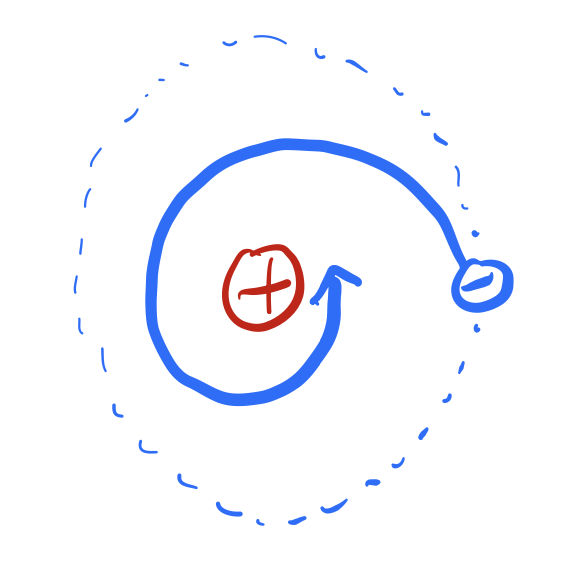
\includegraphics[scale=0.4]{Lectures/Images/lec8-hydrogen.png}
\end{center}

For example, consider a hydrogen atom. In the classical picture, the electron orbits the proton. It then spirals into the proton as it emits radiation (from the effect that we calculate today), and the atom collapses\footnote{And we would be out of drinking water}. But in reality this (fortunately) does not happen, and this is because the radiation emitted from hydrogen atoms are quantized/not continuous. This was one of the confusions of classical physics and was one of the motivations for the development of quantum mechanics.

\begin{center}
    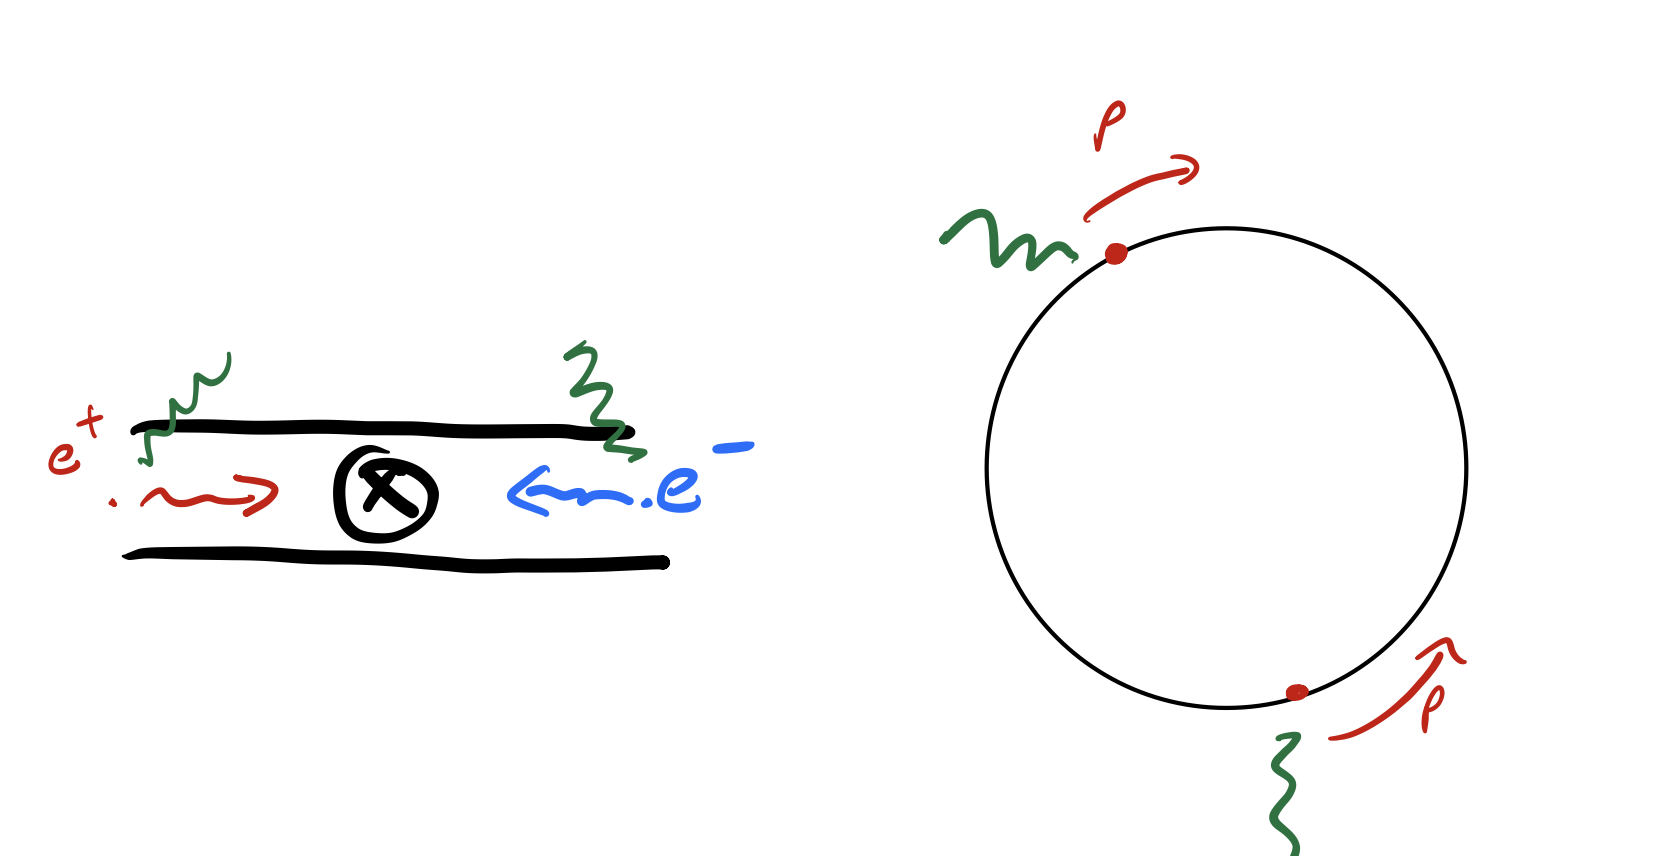
\includegraphics[scale=0.4]{Lectures/Images/lec8-radiation.png}
\end{center}

Another practical example of relevance is accelerators; in either linear or circular accelerators, the accelerating protons/positrons/electrons emit radiation. This is something you have to account for both from an energy efficiency perspective, and also to account for in your signal/measurements as known physics.

\subsection{Calculating fields from charges/currents}
In the last quarter, you saw tha the gauge fields ($\phi, \v{A})$ created by $(\rho, \v{J})$ are given by:
\begin{equation}
    \phi(t, \v{x}) = \frac{1}{4\pi\e_0}\left.\int \frac{d^3\v{x}'}{\abs{\v{x} - \v{x}'}}\rho(t', x')\right|_{\text{ret}}
\end{equation}
\begin{equation}
    \v{A}(t, \v{x}) = \frac{\mu_0}{4\pi}\left.\int \frac{d^3\v{x}'}{\abs{\v{x} - \v{x}'}}\v{J}(t', \v{x}')\right|_{\text{ret}}
\end{equation}

\begin{center}
    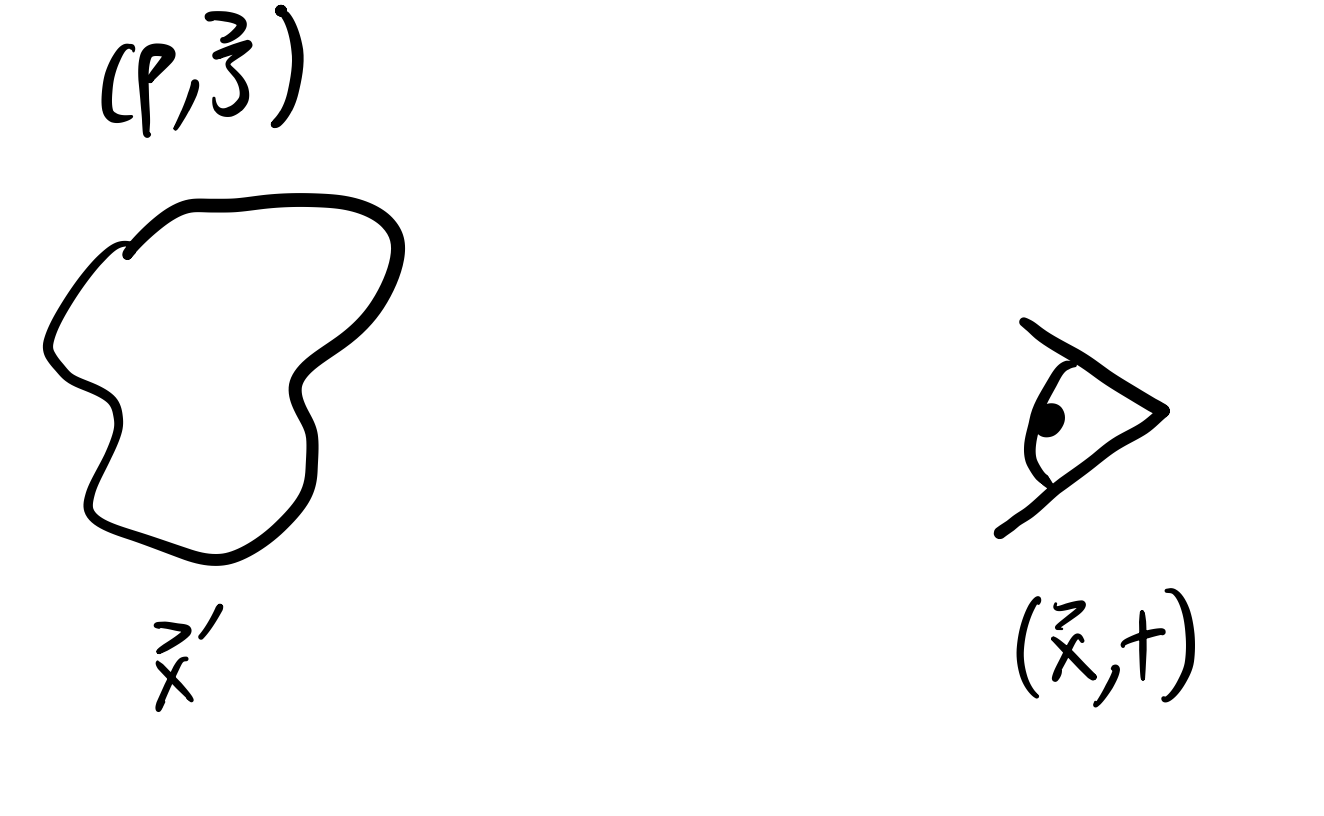
\includegraphics[scale=0.4]{Lectures/Images/lec8-fields.png}
\end{center}

What do these formulas actually say? We integrate over charges/currents at $\v{x}'$, while our location is $\v{x}$ - we evaluate at the retarded time:
\begin{equation}
    t_{\text{ret}} = t' =  t - \frac{1}{c}\abs{\v{x} - \v{x}'}
\end{equation}
which accounts for the locality of the physics - if we move the sources, it takes time for the signal to reach the point $\v{x}$, as the signal is bounded by the speed of light (c.f. the Coloumb force law which acts at a distance).

In terms of the $A_\mu = (-\frac{\phi}{c}, \v{A})$ four vector, we can summarize the above equations as a single one:
\begin{equation}
    A_\mu(t, \v{x}) = \left.\frac{\mu_0}{4\pi}\int \frac{d^3\v{x}'}{\abs{\v{x} - \v{x}'}}J_\mu(t', \v{x}')\right|_{\text{ret}}
\end{equation}

\subsection{Deriving the Leonard-Wiechart Potentials}
Now, we are interested in finding $A_\mu$ for a charged particle is travelling with trajectory $\v{r}(t)$. The charge/current densities are:
\begin{equation}
    \rho(t, \v{x}) = q\delta(\v{x} - \v{r}(t))
\end{equation}
\begin{equation}
    \v{J}(t, \v{x}) = q\dot{\v{r}}\delta(\v{x} - \v{r}(t))
\end{equation}
So we can calculate:
\begin{equation}
    \phi(t, \v{x}) = \frac{q\mu_0 c^2}{4\pi^2}\int \frac{d^3\v{x}'}{\abs{\v{x} - \v{x}'}}\delta(\v{x}' - \v{r}(t_{\text{ret}}))
\end{equation}
\begin{equation}
    \v{A}(t, \v{x}) = \frac{q\mu_0}{4\pi}\int \frac{d^3\v{x}'}{\abs{\v{x} - \v{x}'}}\dot{\v{r}}(t_{\text{ret}})\delta(\v{x}' - \v{r}(t_{\text{ret}}))
\end{equation}
Usually, we would say that the integral of a delta function is quite easy, but here there is a slight complication. The problem is that $\v{r}(t_{\text{ret}})$ depends on $\v{x}'$ through $t_{\text{ret}}$:
\begin{equation}
    \v{t}(t_{\text{ret}}) = \v{r}(t - \frac{1}{c}\abs{\v{x} - \v{x}'})
\end{equation}

To resolve this, let us study the 1-D analog, where we recall the delta function identity:
\begin{equation}
    \int dx g(x) \delta(f(x))  = \left.\frac{g}{\abs{f'}}\right|_{f'=0}
\end{equation}
In 3-D:
\begin{equation}
    \begin{split}
        \int d^3\v{x}g(\v{x})\delta(\v{f}(\v{x})) &= \int d^3\v{x}g(\v{x})\delta(f_1(\v{x}))\delta(f_2(\v{x}))\delta(f_3(\v{x}))
        \\ &= \left.\frac{g}{\abs{J}}\right|_{\v{f}(\v{x}) = 0}
    \end{split}
\end{equation}
where $J$ is the 3x3 matrix:
\begin{equation}
    J^i_{j} = \ddpd{f^i}{x^j}
\end{equation}
and $\abs{J} = \det J$.

With that mathematical aside, let's turn back to our problem. We have:
\begin{equation}
    g(\v{x}) = \frac{1}{\abs{\v{x} - \v{x}'}}
\end{equation}
and:
\begin{equation}
    \v{f}(\v{x}') = \v{x}' - \v{r}(t_{\text{ret}}) = \v{x}' - \v{r}(t - \frac{1}{c}\abs{\v{x} - \v{x}'})
\end{equation}
Calculating $J$\footnote{Kutasov: ``The location of indices are important if you are doing mechanics from Arnold's textbook. If you choose not to subscribe to this, I support you in this decision - they are not that important. Wald may care about this - he may worship at the altar of Arnold, but not me''}:
\begin{equation}
    J^i_j = \ddpd{f^i}{x'^j} = \delta^j_i - \frac{x^j - x'^j}{c\abs{\v{x} - \v{x}'}}\left.\dod{r^i}{t}\right|_{t_\text{ret}}
\end{equation}
To eleborate on this slightly:
\begin{equation}
    \ddpd{}{x'^j}\abs{\v{x} - \v{x}'} = \ddpd{}{x'^j}\left((x_1 - x_1')^2+ (x_2 - x_2')^2 + (x_3 - x_3')^2\right)^{1/2} = \frac{1}{2}\frac{(-1)}{\abs{\v{x} - \v{x}'}}2(x_j - x_j')
\end{equation}
and the full expression we get from that and the chain rule. Evaluating the determinant:
\begin{equation}
    J = \abs{-\frac{\v{x} - \v{x}'}{c\abs{\v{x} - \v{x}'}}\left.\dod{\v{r}}{t}\right|_{t_\text{ret}}}
\end{equation}
Now, if we use this result to evaluate the potentials, we get the Leonard-Wiechart potentials:
\begin{equation}
    \phi(t, \v{x}) = \frac{\mu_0 c^2}{4\pi}\frac{1}{\alpha}\frac{q}{\abs{\v{x} - \v{r}(t_{\text{ret}})}}
\end{equation}
\begin{equation}
    \v{A}(t, \v{x}) = \frac{\mu_0}{4\pi}\frac{1}{\alpha}\frac{q}{\abs{\v{x} - \v{r}(t_{\text{ret}})}}\left.\dod{\v{r}}{t}\right|_{t_\text{ret}}
\end{equation}
Where:
\begin{equation}
    \alpha = 1 -\frac{1}{c}\hat{\v{n}}\cdot \left.\dod{\v{r}}{t}\right|_{t_\text{ret}}
\end{equation}
and:
\begin{equation}
    \hat{\v{n}} = \frac{\v{x} - \v{r}(t_{\text{ret}})}{\abs{\v{x} - \v{r}(t_{\text{ret}})}}
\end{equation}
is the direction from the point we are evaluating the potentials $\v{x}$ to where the particle \emph{was} when we see the signal, assuming the signal travels at the speed of light (hence the evaluation at the retarded time). $t_{\text{ret}}$ implicitly depends on $\v{r}(t_{\text{ret}})$:
\begin{equation}
    t_{\text{ret}} = t - \frac{1}{c}\abs{\v{x} - \v{r}(t_{\text{ret}})}
\end{equation}
and thus solving for this implicitly is the first step of using these potentials. This looks all complicated, but it is all in service of making sure that we do not have action at a distance - physics is local, and it takes time for information to propagate. This hopefully makes the retarded time at least conceptually intuitive.

\begin{center}
    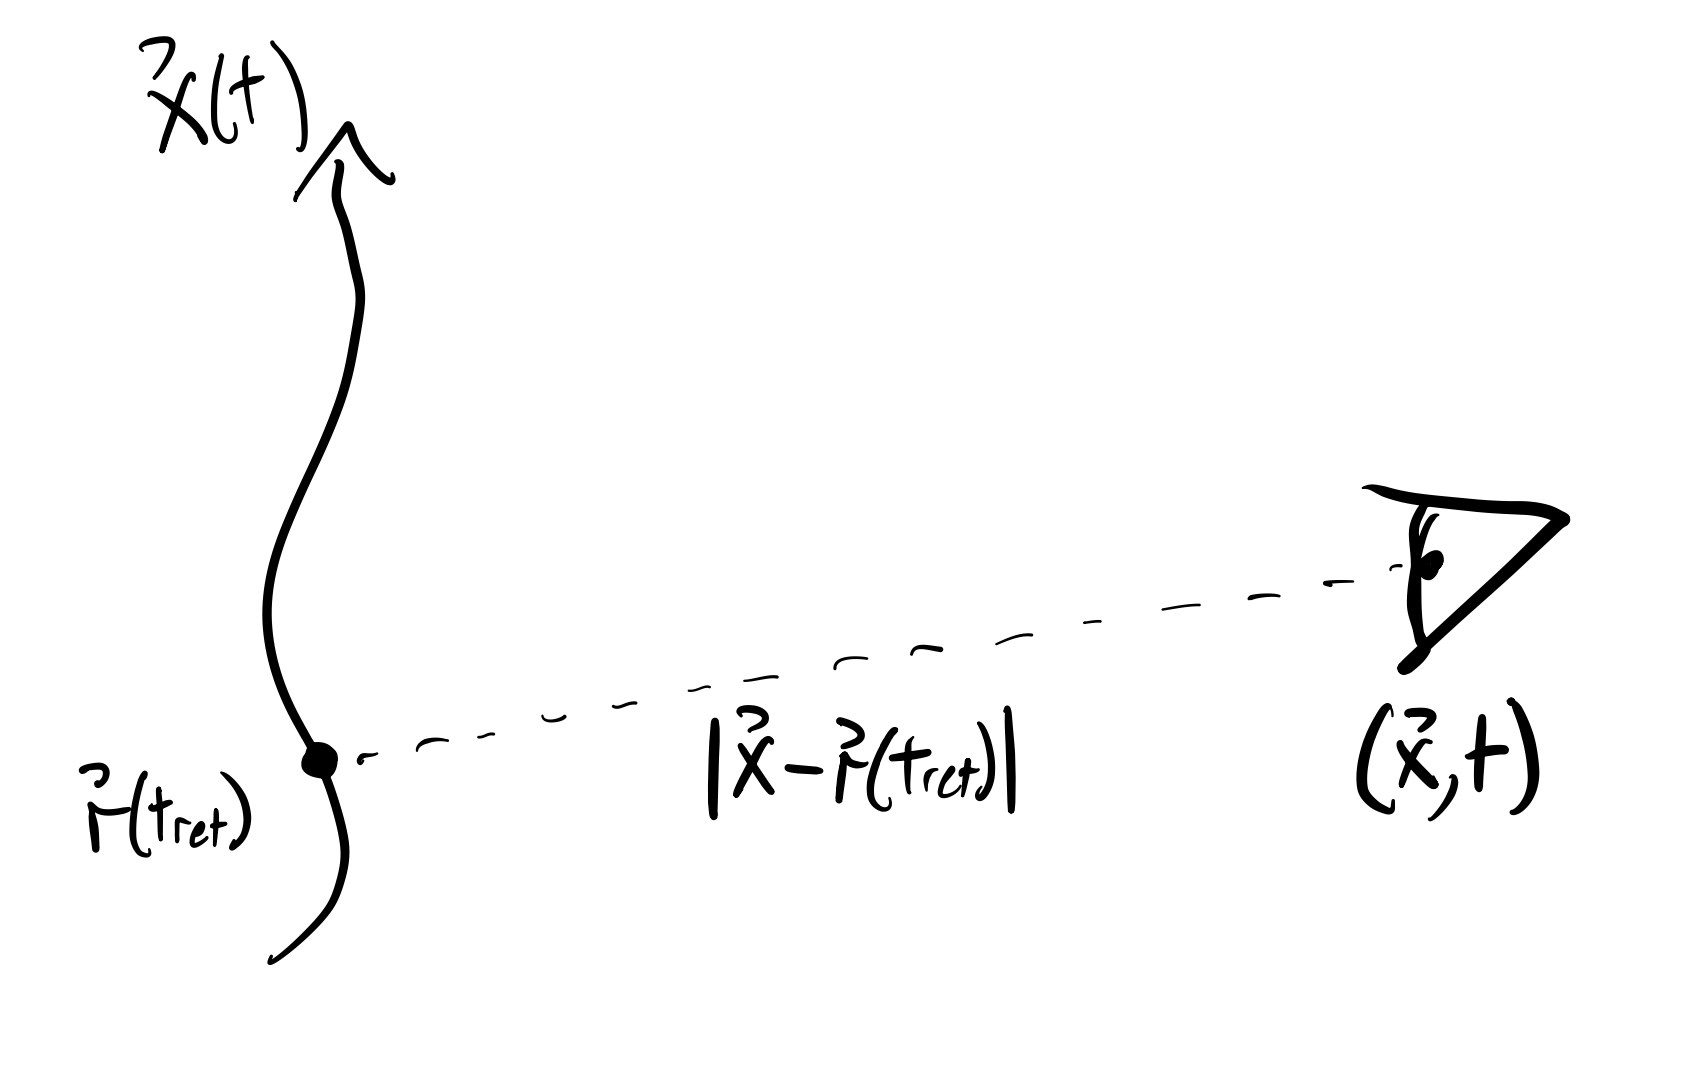
\includegraphics[scale=0.4]{Lectures/Images/lec8-retardedtime.png}
\end{center}

\subsection{Coloumb's Law}
Let $\v{r}(t) = \v{r}_{\text{particle}}$ be a constant/fixed position in space for a particle of charged $q$. Then, we find that $\alpha = 1$, and we get for the potentials:
\begin{equation}
    \phi(t, \v{x}) = \frac{\mu_0 c^2}{4\pi}\frac{q}{\abs{\v{x} - \v{r}_{\text{particle}}}}
\end{equation}
\begin{equation}
    \v{A} = 0
\end{equation}
which is consistent with Coloumb's law. All of the retarded time parts of the expression drops out. But in the case that the particle is accelerating, e.g. we turn on some electric field, the retarded time becomes very important - because we don't see what the particle is doing \emph{now}, but what it was doing some time ago.

\subsection{E/B fields from Leonard-Wiechart Potentials}

We can further ask - what are the $\v{E}, \v{B}$ fields? Normally you could say - look, we have the $A_\mu$, now give it to the graduate student to calculate the fields, but alas you are the graduate students so we must do it. Recall:
\begin{equation}
    \v{E} = -\nabla \phi - \dot{\v{A}}
\end{equation}
\begin{equation}
    \v{B} = \nabla \times \v{A}
\end{equation}
In $\v{E}$ we see the time derivative appear, and so to calculate this we must know:
\begin{equation}
    \dpd{t_{\text{ret}}}{t} = \frac{1}{\alpha}
\end{equation}
you can work through this yourself, see Wald, or see Kutasov's notes for why this is the case. We also will need:
\begin{equation}
    \nabla t_{\text{ret}} = -\frac{1}{\alpha}\hat{\v{n}}
\end{equation}

Now, if we plug in $\phi, \v{A}$ into the expressions for $\v{E}, \v{B}$, we obtain:
\begin{equation}
    \v{E}(t, \v{x}) = q\frac{\mu_0 c^2}{4\pi}\frac{(\hat{\v{n}} - \frac{1}{c}\dod{\v{r}}{t})(1 - \frac{1}{c^2}\left(\dod{\v{r}}{t}\right)^2)}{\alpha^3\abs{\v{x} - \v{r}(t_{\text{ret}})}^2} + q\frac{\mu_0}{4\pi}\frac{\hat{\v{n}} \times [(\hat{\v{n}} - \frac{1}{c}\dod{\v{r}}{t})\times \dod[2]{\v{r}}{t}]}{\alpha^3\abs{\v{x} - \v{r}(t_{\text{ret}})}}
\end{equation}
where all time derivatives are evaluated at the retarded time. The expression for the magnetic field is comparatively simple.
\begin{equation}
   c \v{B}(t, \v{x}) = \hat{\v{n}} \times \v{E}
\end{equation}

and we will analyze these next time - in particular, from the exact expressions above, we will study the radiation we see at spatial infinity. To this end, the first term will not be so important because it is $\frac{1}{x^2}$ (as opposed to the $O(\frac{1}{x})$ term). The first term in $\v{E}$ corresponds to the Coloumb force, the second term (which depends on the acceleration of the particle! key for radiation) gives us a Poynting vector that goes as $O(\frac{1}{x^2})$.
\section{Far-Field Radiation}
Last time, we wrote down the expression for the electromagnetic fields generated by a moving charge with trajectory $\v{r}(t)$:

\begin{equation}
    \v{E}(t, \v{x}) = q\frac{\mu_0 c^2}{4\pi}\frac{(\hat{\v{n}} - \frac{1}{c}\dod{\v{r}}{t})(1 - \frac{1}{c^2}\left(\dod{\v{r}}{t}\right)^2)}{\alpha^3\abs{\v{x} - \v{r}(t_{\text{ret}})}^2} + q\frac{\mu_0}{4\pi}\frac{\hat{\v{n}} \times [(\hat{\v{n}} - \frac{1}{c}\dod{\v{r}}{t})\times \dod[2]{\v{r}}{t}]}{\alpha^3\abs{\v{x} - \v{r}(t_{\text{ret}})}}
\end{equation}
\begin{equation}
    c\v{B}(t, \v{x}) = \hat{\v{n}} \times \v{E}(t, \v{x})
\end{equation}
with:
\begin{equation}
    \alpha = \abs{-\frac{1}{c}\hat{\v{n}}\cdot\dod{\v{r}}{t}(t_{\text{ret}})}, \quad \hat{\v{n}} = \frac{\v{x} - \v{r}(t_{\text{ret}})}{\abs{\v{x} - \v{r}(t_{\text{ret}})}}, \quad t_{\text{ret}} = t - \frac{1}{c}\abs{\v{x} - \v{r}(t_{\text{ret}})}
\end{equation}

\subsection{Poynting Vector and Power}
The reason why this all looks so complicated is that this is the exact result that applies to all cases. You can check that for $\v{r}(t) = \v{x}_0$ that this reduced to the Coloumb field. If $\v{x}(t) = \v{x}_0 + vt$, this reduces to a problem you had in your second problem set (which you can solve via boost). If you were only interested in these two cases, it would be madness to calculate the general case and restrict after, but we are interested in slightly more sophisticated scenarios. In particular, we want to study radiation. As you learned in the last quarter, the hero of the story is the Poynting vector:
\begin{equation}
    \v{S} = \frac{1}{\mu_0}\v{E} \times \v{B}
\end{equation}

We are interested in looking at the radiation a large distance from the source, and hence the $\frac{1}{x^2}$ (with $x = \abs{\v{x} - \v{r}(t_{\text{ret}})} \approx \abs{\v{x}}$.

\begin{center}
    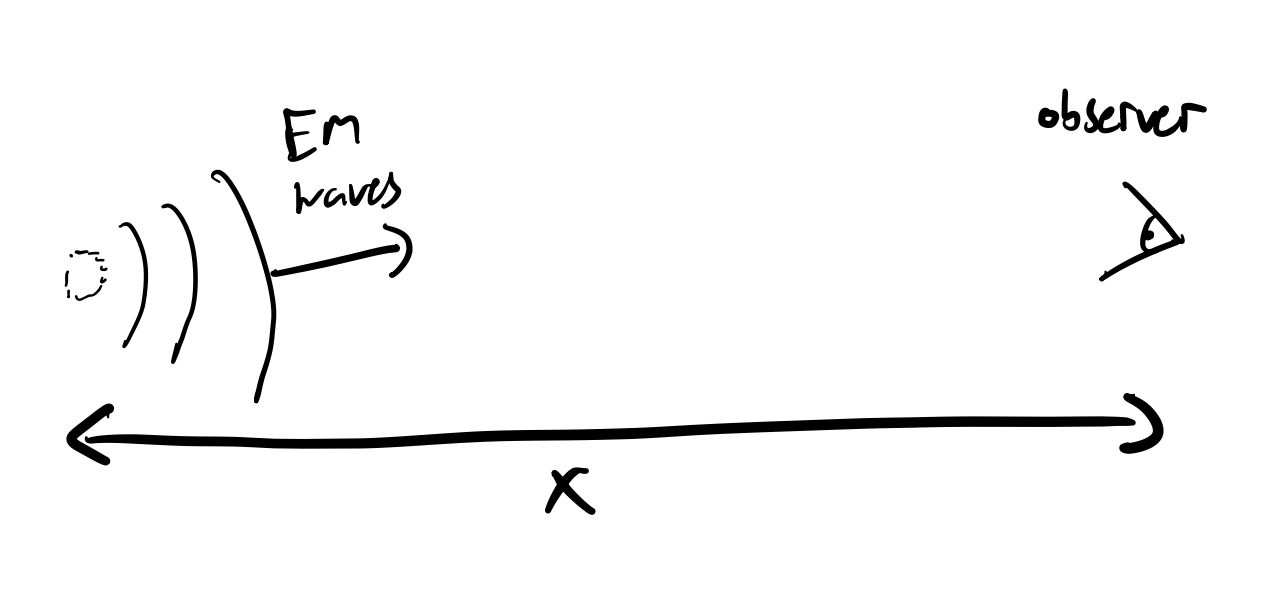
\includegraphics[scale=0.38]{Lectures/Images/lec9-farfield.png}
\end{center}

We take the particle motion to be approximately confined to the origin) contributions to $\v{S}$ (all higher order terms we will drop). Looking at $\v{E}/\v{B}$, we have two terms:
\begin{equation}
    \v{E} \sim \frac{1}{x^2} + \frac{1}{x}
\end{equation}
\begin{equation}
    \v{B} \sim \v{E} \sim \frac{1}{x^2} + \frac{1}{x}
\end{equation}
So when we calculate $\v{S}$ by taking their cross product, the leading contribution will come from the product of the two $\frac{1}{x}$ terms.

For a given solid angle $d\Omega$, what is the power (energy/time) $dP$ that goes into it? 

\begin{center}
    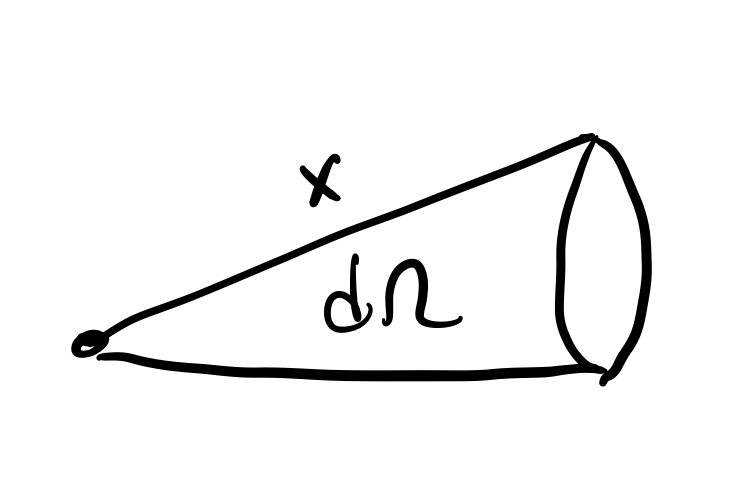
\includegraphics[scale=0.38]{Lectures/Images/lec9-solidangle.png}
\end{center}

Recall from last quarter that:
\begin{equation}
    \dod{P}{\Omega} = \lim_{\v{x} \to \infty}\abs{\v{x}}^2\v{S} \cdot \hat{\v{x}}
\end{equation}
Be aware that the $P$ above is not the same as the momentum density of the field:
\begin{equation}
    \v{P} = \e_0 \v{E} \times \v{B}
\end{equation}

For us, the power per solid angle is given (after only retaining terms of $\frac{1}{x^2}$):
\begin{equation}\label{eq:powerpersolidangle}
    \dod{P}{\Omega} = \frac{q^2\mu_0}{16\pi^2c\alpha^6}\abs{\hat{\v{x}}\times\left[\left(\hat{\v{x}} - \frac{1}{c}\dod{\v{r}}{t}\right) \times \dod[2]{\v{r}}{t}\right]}^2
\end{equation}
where the time derivatives are evaluated at $t_{\text{ret}}$, which reduces to:
\begin{equation}
    t_{\text{ret}} = t - \frac{1}{c}\abs{\v{x}}
\end{equation}
after taking $\v{x} \gg \v{r}$. Note from Eq. \eqref{eq:powerpersolidangle} that if we have no acceleration, then we have no radiation.

Note that we can write down a related quantity $\od{P'}{\Omega}$, with $P'$ the energy per unit retarded time (the energy seen by the emitter):
\begin{equation}
    \dod{P'}{\Omega} = \dod{P}{\Omega}\dod{t}{t_{\text{ret}}} = \dod{P}{\Omega} \alpha = \frac{q^2\mu_0}{16\pi^2c\alpha^5}\abs{\hat{\v{x}}\times\left[\left(\hat{\v{x}} - \frac{1}{c}\dod{\v{r}}{t}\right) \times \dod[2]{\v{r}}{t}\right]}^2
\end{equation}
In other words, if we know how to calculate one, we can easily obtain the other.

\subsection{Nonrelativistic Limit \& Connection to Dipoles}
Note that even though the particle is accelerating, we can put ourselves in a frame where $\od{\v{x}}{t} = \v{0}$ (more specifically, we can consider that the particle is moving sufficiently slowly that $\frac{1}{c}\od{\v{x}}{t} \ll 1$) instantaneously at $t_{\text{ret}}$. Then:
\begin{equation}
    \alpha = 1 - \frac{1}{c}\hat{\v{n}}\cdot\dod{\v{x}}{t}(t_{\text{ret}}) = 1
\end{equation}
In this case, we can write down a simpler looking formula:
\begin{equation}
    \left.\dod{P'}{\Omega}\right|_{\od{\v{x}}{t}=0} = \frac{q^2\mu_0}{16\pi^2c}\abs{\hat{\v{x}}\times\left[\hat{\v{x}} \times \dod[2]{\v{r}}{t}\right]}^2
\end{equation}
An interpretation is that the above formula corresponds to the power radiated from a particle accelerating from rest. Using vector identities, we can write it as:
\begin{equation}\label{eq:powerpersolidanglenonrel}
    \left.\dod{P'}{\Omega}\right|_{\od{\v{x}}{t}=0} = \frac{q^2\mu_0}{16\pi^2c}\left(\abs{\dod[2]{\v{r}}{t}}^2 - \abs{\hat{\v{x}} \cdot \dod[2]{\v{r}}{t}}^2\right)
\end{equation}

Recall back to last quarter, where you looked at the time-dependent dipole (with moment $\v{p}$):
\begin{equation}\label{eq:dipoleS}
    \v{S} = \frac{\mu_0\hat{\v{x}}}{16\pi^2 c\abs{\v{x}}^2}\left[\abs{\dod[2]{\v{p}}{t}}_{t_{\text{ret}}}^2 - \left.\left(\hat{\v{x}} \cdot \dod[2]{\v{p}}{t}\right)^2\right|_{t_{\text{ret}}} \right]
\end{equation}
We notice that this looks strikingly similar to the formula we have derived. This is no coincidence. Let's think about the dipole moment:
\begin{equation}
    \v{p} = \int d^3\v{x}\rho(\v{x})\v{x}
\end{equation}
The particle we are dealing with can be thought of:
\begin{equation}
    \rho(\v{x}) = q\delta(\v{x} - \v{r}(t))
\end{equation}
which has the dipole moment:
\begin{equation}
    \v{p} = q\v{r}(t)
\end{equation}
and now we're in business - if we plug this into Eq. \eqref{eq:dipoleS} we will recover the power per solid angle of Eq. \eqref{eq:powerpersolidanglenonrel}.

We can also ask: How does $\od{P}{\Omega}$ depend on the angle $\vartheta$ between the acceleration of the source and the observation point? 

\begin{center}
    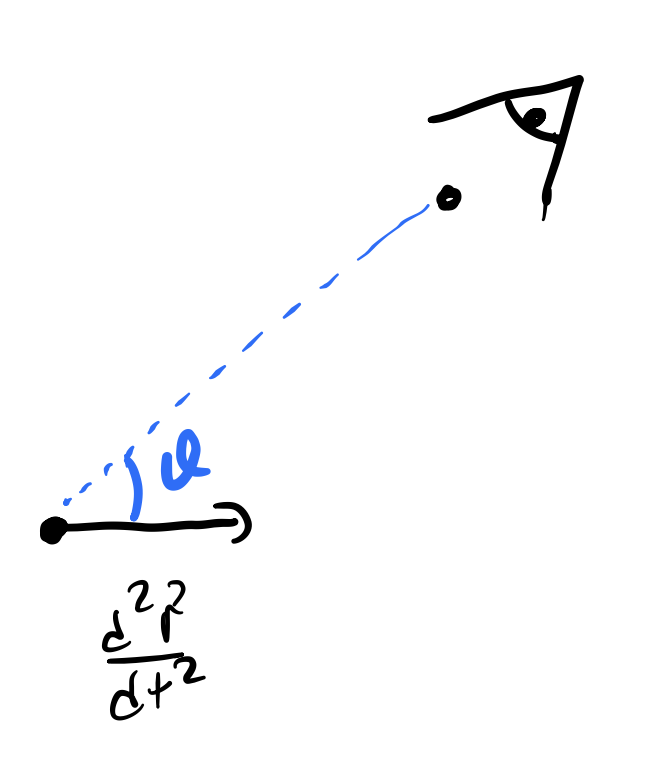
\includegraphics[scale=0.38]{Lectures/Images/lec9-accelangle.png}
\end{center}

It is the same answer as you found for the dipole last quarter:

\begin{equation}
    \dod{P}{\Omega} \propto \sin^2\vartheta
\end{equation}

\subsection{Relativistic Case - Special Limits}
What if we go away from the nonrelativistic limit - therein we consider a velocity:
\begin{equation}
    \dod{\v{r}}{t}(t_{\text{ret}}) = v\zhat
\end{equation}
where $\frac{v}{c}$ is no longer small. Letting $\theta$ be the polar angle

\begin{center}
    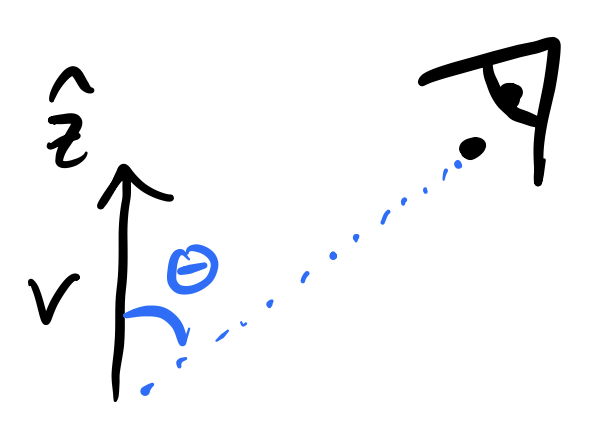
\includegraphics[scale=0.38]{Lectures/Images/lec9-velocangle.png}
\end{center}

We can take:
\begin{equation}
    \alpha = 1 - \frac{v}{c}\cos\theta
\end{equation}

Let us consider two special cases:
\begin{itemize}
    \item $\od[2]{\v{r}}{t}, \od{\v{r}}{t}$ are parallel. This is the case, e.g., in a linear accelerator. In that case we have:
    \begin{equation}
        \left(\dod{P}{\Omega}\right)_{\parallel} = \frac{q^2\mu_0}{16\pi^2 c}\frac{\sin^2\theta}{(1 - \frac{v}{c}\cos\theta)^6}\abs{\dod[2]{\v{r}}{t}}^2
    \end{equation}
    \begin{equation}
        \left(\dod{P'}{\Omega}\right)_{\parallel} = \frac{q^2\mu_0}{16\pi^2 c}\frac{\sin^2\theta}{(1 - \frac{v}{c}\cos\theta)^5}\abs{\dod[2]{\v{r}}{t}}^2
    \end{equation}
    Note that since the acceleration/velocity are perpendicular, $\vartheta = \theta$ and hence the two angles appearing in the above are the same.
    \item  $\od[2]{\v{r}}{t}$ and $\od{\v{r}}{t}$ are perpendicular. This is the case, e.g., when a particle is moving in a circle, where the acceleration points into the center and the velocity points tangent to the circle. In this case, we find:
    \begin{equation}
        \left(\dod{P}{\Omega}\right)_{\perp} = \frac{q^2\mu_0}{16\pi^2 c}\frac{1}{(1-\frac{v}{c}\cos\theta)^2}\abs{\dod[2]{\v{x}}{t}}^2\left[(1 - \frac{v}{c}\cos\theta)^2 - (1 - \frac{v^2}{c^2})\sin^2\theta\cos^2\phi\right]
    \end{equation}
    Where $\theta, \phi$ are the Euler angles (polar and azimuthal angle of the observer relative to the velocity and acceleration... I think).
\end{itemize}

A remark - in the $v \to c$ limit, the power is concentrated in the forwards direction.


\subsection{Larmor Formula and Generalization}
When designing an accelerator, we want to know the total power that gets radiated. This can be calculated by integrating over all solid angles:
\begin{equation}
    P = \int d\Omega \dod{P}{\Omega} = \int \sin\theta d\theta d\phi \dod{P}{\Omega}
\end{equation}
In particular in the limit that $v \ll c$, you saw last quarter (p.84 in Wald) that:
\begin{equation}
    P_0 =  \frac{q^2\mu_0}{6\pi c}\abs{\dod[2]{\v{r}}{t}}^2_{\text{ret}}
\end{equation}
This is an interesting formula, because we can calculate the energy that gets lost over the period of acceleration (assuming the particle does not approach relativistic speeds, for $P_0$). We can analyze the units:
\begin{equation}
    \frac{E}{T} = P = \frac{q^2 \mu_0}{c}\left(\frac{L}{T^2}\right)^2
\end{equation}
from Coloumb we know that:
\begin{equation}
    E = \frac{1}{\e_0}\frac{q^2}{L} = \frac{q^2\mu_0}{c^2}\frac{1}{L}
\end{equation}
and so we find:
\begin{equation}
    c^3 = \frac{L^3}{T^3}
\end{equation}
so the dimensions check out. This is a useful check of your results, e.g. on your midterm if you have time.

To generalize the Larmor formula, we have to consider finite $\frac{v}{c}$. Either we can redo the entire calculation with all the factors of $v$ we neglected. But there is a quicker way; that is to note two things:
\begin{itemize}
    \item $P$ is a Lorentz scalar
    \item $P$ only depends on $\v{v}, \dot{\v{v}}$.
\end{itemize}
The second expression is obvious. The first is a little more subtle, you can see it in Wald 183, but it has to do with the fact that:
\begin{equation}
    P = \dod{E}{t}
\end{equation}
and both $E, t$ are zeroth components of four-vectors. With these two facts, we find that the analog of the total power is:
\begin{equation}
    P = \frac{q^2\mu_0}{6\pi c}\gamma^6\left[\abs{\dot{\v{v}}}^2 - \left(\frac{\v{v} \times \dot{\v{v}}}{c}\right)^2\right]
\end{equation}
Next time, we have 20 minutes more discussion on this topic, and that concludes the midterm coverage.
\section{Linear/Circular Accelerators, Radiation from Continuous Sources I}

\subsection{Linear/Circular Accelerators}
Last time we derived the generalization of the Larmor formula:
\begin{equation}
    P = \frac{q^2\mu_0}{6\pi c}\gamma^6\left[\abs{\dot{\v{v}}}^2 - \left(\frac{\v{v} \times \dot{\v{v}}}{c}\right)^2\right]_{\text{ret}}
\end{equation}
with $\gamma = \frac{1}{\sqrt{1- \frac{\abs{\v{v}}^2}{c^2}}}$ the familiar Lorentz factor. Let us study the two cases:
\begin{itemize}
    \item $\v{v} \parallel \dot{\v{v}}$ (relevant for linear accelerators). In this case, we have that $\v{v} \times \dot{\v{v}} = \v{0}$, so the formula simplifies to:
    \begin{equation}\label{eq:powerparallel}
        P = \frac{q^2\mu_0}{6\pi c}\gamma^6\abs{\dot{\v{v}}}^2
    \end{equation}

    The structures appearing here can be naturally written in terms of the change in (relativistic) momentum $p = m\gamma v$:
    \begin{equation}
        \dod{p}{t} = m\dod{}{t}(\gamma v) = m\dod{}{t}\left(\frac{v}{\sqrt{1 - \frac{v^2}{c^2}}}\right) = m\gamma^3\dot{v}
    \end{equation} 
    We can thus write Eq. \eqref{eq:powerparallel} in terms of the rate of change of momentum:
    \begin{equation}
        P = \frac{q^2\mu_0}{6\pi c m^2}\left(\dod{p}{t}\right)^2
    \end{equation}
    How do we interpret this? Well, recall the particle satisfies the dispersion relation:
    \begin{equation}
        E^2 = p^2c^2 + (mc^2)^2 = m \gamma c^2
    \end{equation}
    We find from the above that, in the linear case:
    \begin{equation}
        \dod{p}{t} = \dod{E}{x}
    \end{equation}
    where we parametrize the particle energy at position $E(x)$. If we make this replacement:
    \begin{equation}
        P = \frac{q^2\mu_0}{6\pi c m^2}\left(\dod{E}{x}\right)^2
    \end{equation}
    This is much more visual. The whole reason why we made this accelerator is to accelerate particles, and we only have a finite amount of real estate to do this. We therefore want the rate of change of the energy of the particle to be as large as possible. But then we pay the price in radiation\footnote{There is no such thing as a free lunch. There is such a thing as a very expensive lunch.}.

    \item $\v{v} \perp \dot{\v{v}}$ (relevant for circular accelerators). In this case, the cross product of the velocity/acceleration is just the product of the magnitudes, so $\abs{\v{v} \times \dot{\v{v}}}^2 = \abs{\v{v}}^2\abs{\dot{\v{v}}}^2$ and so:
    \begin{equation}
        P = \frac{q^2\mu_0}{6\pi c}\gamma^4\abs{\dot{\v{v}}}^2
    \end{equation}
    Compare the $\gamma^4$ to the $\gamma^6$ for the linear accelerators. But, in the circular case, we pay the price of $\gamma^4$ even if the particle does not accelerate - it costs energy to just keep the particle moving around. In particular, we can ask - how much energy is lost per revolution\footnote{One time around the circle, not the communist revolution}?

    For radius $\rho$, can write the period as:
    \begin{equation}
        T = \frac{2\pi \rho}{v} = \frac{2\pi \rho}{c\beta}
    \end{equation}
    the acceleration is then:
    \begin{equation}
        a = \frac{v^2}{\rho}
    \end{equation}
    And we find:
    \begin{equation}
        \Delta E = TP = \frac{1}{3}q^2\mu_0 \gamma^4\frac{v^3}{\rho}
    \end{equation}
    In the LHC, the charged particles are protons, and the radius is $\rho \sim 27\si{km}$. The mass of the protons are:
    \begin{equation}
        m_P c^2 \sim 1\si{GeV}
    \end{equation}
    The energies the protons are accelerated to are:
    \begin{equation}
        E \sim 10\si{TeV} = 10000\si{GeV}
    \end{equation}
    So:
    \begin{equation}
        E = m_p \gamma c^2 \implies \gamma = \frac{E}{m_p c^2} = 10000
    \end{equation}
    In this limit, $v \sim c$ and so:
    \begin{equation}
        \Delta E = \frac{1}{3}q^2\mu_0 \gamma^4\frac{c^3}{\rho} \sim 2.2\si{keV}
    \end{equation}
    Note that this is \emph{not} the energy lost to radiation while accelerating the protons, but rather the energy lost per revolution after they are already brought up to speed. You might say that the 2.2keV looks puny in comparison to the 10TeV energy. But you have to remember that every second, the protons do 10000 revolutions. Therefore, each second we lose 22MeV, and we must inject this amount of energy if we do not want the protons to slow down. This operates 8-10 hours a day, and there is more than 1 proton in the system... it is not our job here, but if you go into designing accelerators in the future, this is something you will need to think about.
    \end{itemize}

\begin{center}
    \emph{End of midterm content.}
\end{center}

\subsection{Solving Maxwell for continuous sources}
Consider now the continuous distributions $\rho(\v{x}, t), \v{J}(\v{x}, t)$. The question we want to discuss is simple - somebody hands you the above, and you want to solve the Maxwell equations with these sources. A good discussion of the 

A couple comments:
\begin{itemize}
    \item We are dealing with linear differential equations, and thus the general solution with a given source $J^\mu(x)$ is the same as any particular solution $A_\mu^{p}(x)$ with the source + the general solution of the homogenous equation/source-free case $A_\mu^{\text{free}}(x)$.
    \item If $A_\mu^{(1)}$ is a solution for source $J_\mu^{(1)}$ and $A_\mu^{(2)}$ is a solution for source $J_\mu^{(2)}$, then $A_\mu^{(1)} + A_\mu^{(2)}$ is a solution for source $J_\mu^{(1)} + J_\mu^{(2)}$.
\end{itemize}
These two observations simplifies things considerably. Namely, it suffices to consider:
\begin{equation}
    \rho(\v{x}, t) \stackrel{?}{=} \rho(\v{x})\exp(-i\omega t)
\end{equation}
There are some points to make. First, the $\rho$s appearing on different sides of the equation are different functions, but we will have to accept such abuse of notation. Second, the RHS is complex, so we really have to take the real part:
\begin{equation}
    \rho(\v{x}, t) = \Re(\rho(\v{x})\exp(-i\omega t))
\end{equation}
Back to the central point - why can we generically write things this way? Well, consider the Fourier transform:
\begin{equation}
    \rho(\v{x}, t) = \frac{1}{2\pi}\int d\omega \tilde{\rho}(\v{x}, \omega)e^{i\omega t}
\end{equation}
then the fact that we can take linear superpositions of solutions tells us that it suffices to look at $\Re(\rho(\v{x})\exp(-i\omega t))$. Similarly, we consider:
\begin{equation}
    \v{J}(x) = \v{J}(\v{x}, t) = \Re(\v{J}(\v{x})e^{-i\omega t})
\end{equation}
If we plug these into the continuity equation:
\begin{equation}
    \p_t \rho + \nabla \cdot \v{J} = 0
\end{equation}
then:
\begin{equation}
    i\omega \rho(\v{x}) = \nabla \cdot \v{J}(\v{x})
\end{equation}

We can now obtain the vector potential:
\begin{equation}
    \v{A}(x) = \frac{\mu_0}{4\pi}\int d^4x' \frac{\v{J}(x')}{\abs{\v{x} - \v{x}'}}\delta(t' - t + \frac{\abs{\v{x} - \v{x}'}}{c})
\end{equation}
And analogous for $\phi$. We remark that this vanishes if $\v{J} = \v{0}$, which is not true for the general solution - it is just a particular solution. When we write down the above, we are fixing the freedom in $\v{A}$, and saying that we are only interested in the vector potential that arises from the sources of interest.

The time part of the integral is very simple, because we only get a contribution from the delta function:
\begin{equation}\label{eq:Aintegral}
    \v{A}(\v{x}) = \frac{\mu_0}{4\pi}\int d^3\v{x}'\v{J}(\v{x}')\frac{e^{ik\abs{\v{x} - \v{x}'}}}{\abs{\v{x} - \v{x}'}}
\end{equation}
with $k = \omega/c$. We have also made the same replacement that $\v{A}(x) = \v{A}(\v{x})e^{-i\omega t}$ in the above so the dependence drops out. Now writing down the field:
\begin{equation}
    \v{H} = \frac{1}{\mu_0}\v{B} = \frac{1}{\mu_0}\nabla \times \v{A} 
\end{equation}
and $\v{E}$ we obtain as:
\begin{equation}
    \v{E} = \frac{iZ_0}{k}\nabla \times \v{H}
\end{equation}
with:
\begin{equation}
    Z_0 = \sqrt{\frac{\mu_0}{\e_0}}
\end{equation}
the impedance of the vacuum.

Presumably, there is some finite region in space where the source $J^\mu$ is nonzero. The integral over $\v{x}'$ in Eq. \eqref{eq:Aintegral} therefore is actually over a finite region. One scale that appears is $d$ (the size of the distribution) and another is the wavelength $\lambda = \frac{2\pi}{k}$, which governs the length over which the exponent varies. Finally, there is a third scale $r = \abs{\v{x}}$ which is the distance from the source to the detector.

\begin{center}
    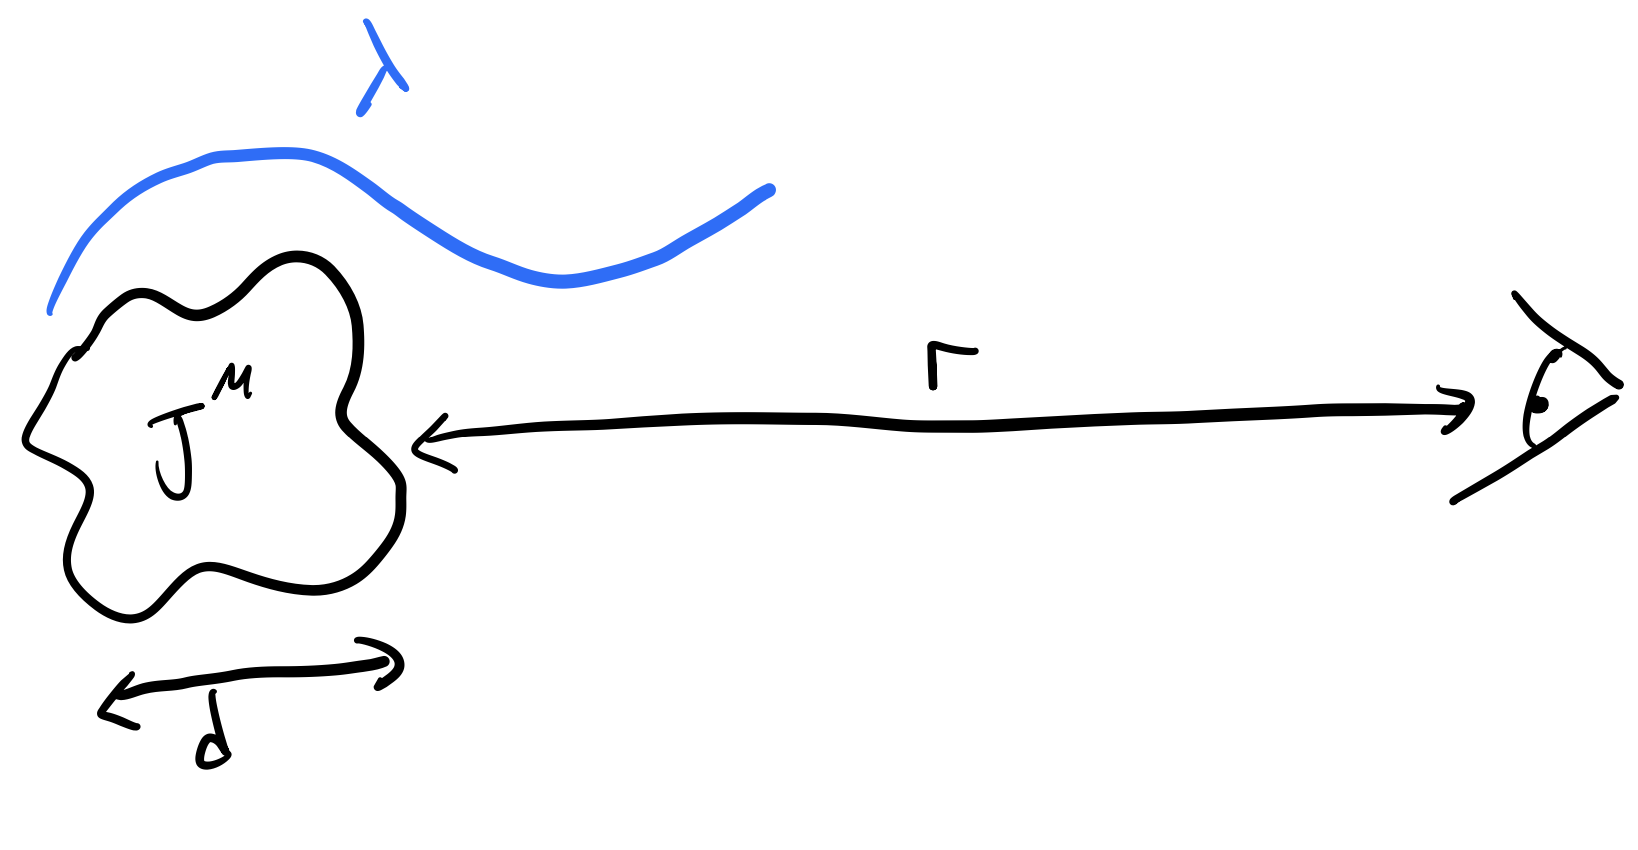
\includegraphics[scale=0.35]{Lectures/Images/lec10-lambdard.png}
\end{center}

Because we have only so much time, we assume $d \ll \lambda$. There are then two limits to consider, the near-field region $d \ll r \ll \lambda$ and the far-field region $d \ll \lambda \ll r$ (the intermediate cases are the most complicated):

\begin{center}
    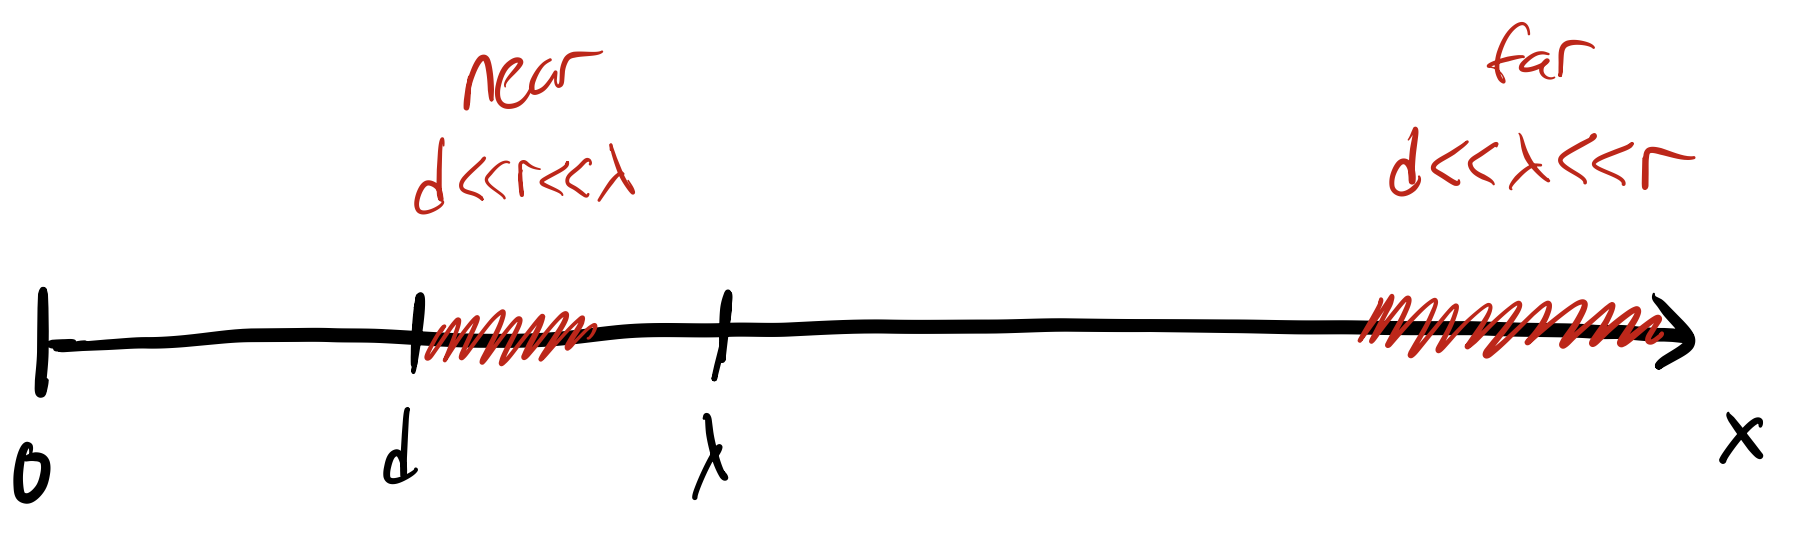
\includegraphics[scale=0.35]{Lectures/Images/lec10-nearfar.png}
\end{center}

In the near-field region, $e^{ik\abs{\v{x} - \v{x}'}} \approx 1$, because $\abs{\v{x} - \v{x}'}$ never goes to scales above $\lambda$. In this limit, the integral becomes simple:
\begin{equation}
    \v{A}(\v{x}) = \frac{\mu_0}{4\pi}\int d^3\v{x}'\frac{\v{J}(\v{x'})}{\abs{\v{x} - \v{x}'}}
\end{equation}
which is the static case which you studied in PHYS 322. This limit is not interesting to us, because we are trying to study radiation from this source. What about the far-field limit? In this limit, we might want to say we can erase the $\v{x}'$ in the denominator and numerator. This is half right; we can omit it in the denominator, but not in the numerator. Let's see why this is.

\begin{center}
    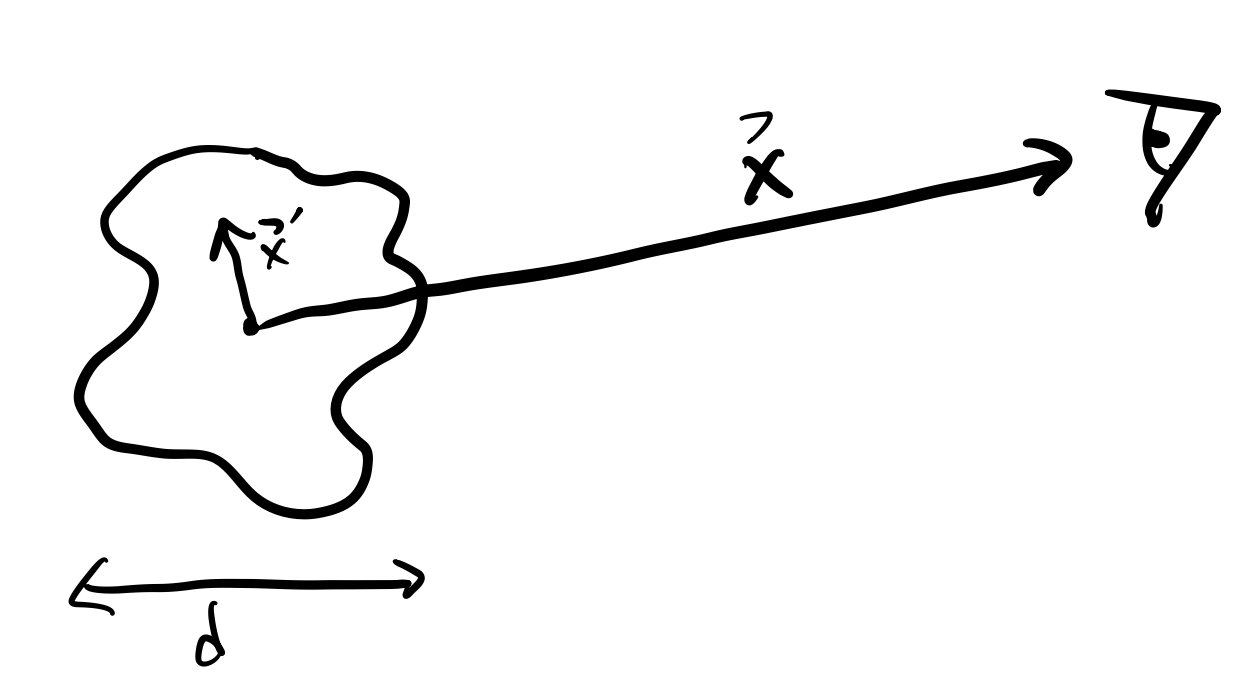
\includegraphics[scale=0.35]{Lectures/Images/lec10-rrprime.png}
\end{center}

Let's study $\abs{\v{x} - \v{x}'}^2$:
\begin{equation}
    \abs{\v{x} - \v{x}'} = \abs{\v{x}}^2 - 2\v{x} \cdot \v{x}' + \abs{\v{x}'}^2
\end{equation}
The last term can indeed be neglected as it is $O(d^2)$ while the other terms are $O(r^2), O(r)$; writing $\v{x} = r\hat{\v{n}}$, we have:
\begin{equation}
    \abs{\v{x} - \v{x}'}^2 \sim r^2 - 2r\hat{\v{n}} \cdot \v{x}' 
\end{equation}
and so:
\begin{equation}
    \abs{\v{x} - \v{x}'} = r - \hat{\v{n}} \cdot \v{x}' + O(\frac{1}{r})
\end{equation}
Then:
\begin{equation}
    \v{A}(\v{x}) = \frac{\mu_0}{4\pi}\frac{e^{ikr}}{r}\int d^3\v{x}' \v{J}(\v{x'})e^{-ik\hat{\v{n}}\cdot\v{x}'}
\end{equation}
The first observation; if we look at the prefactor $\frac{e^{ikr}}{r}$, we find that $\v{A} \sim \frac{1}{r}$, so $\v{E}, \v{B} \sim \frac{1}{r}$ and so the Poynting vector at leading order goes as $\frac{1}{r^2}$, which is the appropriate form for having finite radiation. Pictorially, it looks like an outgoing spherical wave. If we look at the second/integral term, this is $O(1)$ as there is no $r$ dependence. But, it is not negligible - it \emph{does} have angular dependence. The answer will depend on the direction we put our detector $\hat{\v{n}} = \hat{\v{n}}(\theta, \phi)$. Depending on the current distribution, we get different values for the angles $\theta, \phi$. Our task for next time is to finish analyzing this far-field result.
\section{Radiation from Continuous Sources II}

\subsection{Review of Continuous Distribution Maxwell Solutions}

\begin{center}
    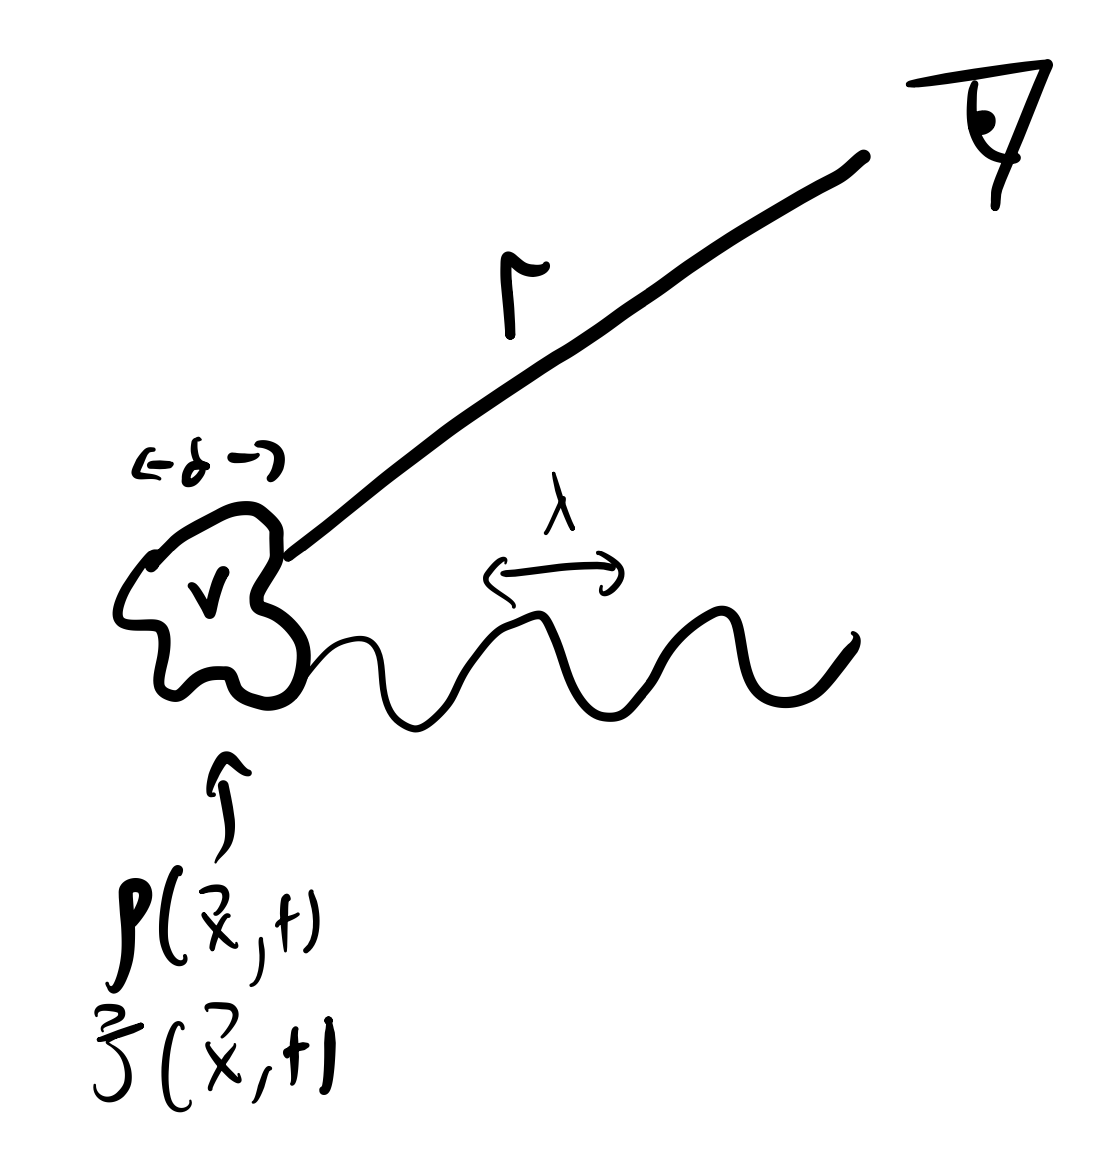
\includegraphics[scale=0.35]{Lectures/Images/lec11-continoussourceradiation.png}
\end{center}

Since Maxwell's equations are linear, we can fourier transform in time and take:
\begin{equation}
    \rho(\v{x}, t) = \rho(\v{x})e^{i\omega t}
\end{equation}\begin{equation}
    \v{J}(\v{x}, t) = \v{J}(\v{x})e^{i\omega t}
\end{equation}
And with the continuity equation:
\begin{equation}
    \dot{\rho} + \nabla \cdot \v{J} = 0
\end{equation}
the two are related by:
\begin{equation}
    i\omega \rho(\v{x}) = \nabla \cdot \v{J}(\v{x})
\end{equation}

Npw, solving Maxwell's equation with these sources, we have:
\begin{equation}
    \v{A}(\v{x}) = \frac{\mu_0}{4\pi}\int d^3\v{x}'\v{J}(\v{x}')\frac{e^{ik\abs{\v{x} - \v{x}'}}}{\abs{\v{x} - \v{x}'}}
\end{equation}
with $k = \frac{\omega}{c} = \frac{2\pi}{\lambda}$. $A_0$ is fixed by the Lorentz gauge condition. From these we get the EM fields:
\begin{equation}
    \v{H} = \frac{1}{\mu_0}\v{B} = \frac{1}{\mu_0}\nabla \times \v{A}
\end{equation}
\begin{equation}
    \v{E} = \frac{iZ_0}{k}\nabla \times \v{H}
\end{equation}
with $Z_0 = \sqrt{\frac{\e_0}{\mu_0}}$.

We studied the long wavelength limit $\lambda \gg d$, and discussed the different regimes where we could place our detector; the near field is where $\abs{\v{x}} \sim d$, the intermediate field is where $\abs{\v{x}} \sim \lambda$, and the far field where $\abs{\v{x}} \gg \lambda$. In this far-field regime:
\begin{equation}
    \v{A}(\v{x}) = \frac{\mu_0}{4\pi}\frac{e^{ikr}}{r}\int_V d^3\v{x}'\v{J}(\v{x}')e^{-ik\hat{\v{n}}\cdot\v{x}'}
\end{equation}
with $r = \abs{\v{x}}$. There is no $r$ dependence left in the integral, but there is an angular dependence through $\hat{\v{n}}\cdot\v{x}'$. In particular this integral depends on $d, \lambda, \theta, \phi$.

\subsection{The Electric Dipole Approximation}
How do we analyze this integral? We can do a power series in the exponential, and get a power series in $\frac{d}{\lambda}$. Doing this:
\begin{equation}
    \int d^3\v{x}' \v{J}(\v{x}')e^{-ik\hat{\v{n}}\cdot\v{x}'} = \sum_{j=0}^\infty \frac{(-ik)^j}{j!}\int d^3\v{x}' \v{J}(\v{x}')(\hat{\v{n}} \cdot \v{x}')^j
\end{equation}
Looking at $j = 0$ - this is the electric dipole approximation:
\begin{equation}
    \v{A}(\v{x}) = \frac{\mu_0}{4\pi}\frac{e^{ikr}}{r}\int d^3\v{x}'\v{J}(\v{x}')
\end{equation}
Why is it called this? Indeed, if we consider:
\begin{equation}
    \gv{\theta} = \int d^3\v{x}' \v{x}(\nabla \cdot \v{J}(\v{x}')) = -\int d^3\v{x}' \v{J}(\v{x}')
\end{equation}
Where in the last equality we have used integration by parts. We also have assumed that the boundary terms vanish - we are in fact interested in the setting where if we exit the region of the source, the currents go to zero. On the other hand, we can replace $\nabla \cdot \v{J}(\v{x}') = i\omega \rho(\v{x}')$ by the continuity equation. With this in mind, let us rewrite the vector potential as:
\begin{equation}
    \v{A}(\v{x}) = -\frac{i\mu_0\omega}{4\pi}\v{p}\frac{e^{ikr}}{r}
\end{equation}
with:
\begin{equation}
    \v{p} = \int d^3\v{x}' \v{x}'\rho(\v{x}')
\end{equation}
So we now understand why this is called the dipole approximation - a time dependent dipole gives rise to this vector potential. From this, we get the magnetic field (as you will check on the problem set):
\begin{equation}
    \v{H} = \frac{ck^2}{4\pi}\hat{\v{n}} \times \v{p}\frac{e{^ikr}}{r}
\end{equation}
and the electric field:
\begin{equation}
    \v{E} = Z_0\v{H} \times \hat{\v{n}}
\end{equation}
There is a nice picture here, namely that the electric field, magnetic field, and $\hat{\v{n}}$ are all perpendicular. EM waves are transverse. From this, we can find the power per solid angle:
\begin{equation}
    \dod{P}{\Omega} = \frac{c^2Z_0}{32\pi^2}k^4\abs{(\hat{\v{n}} \times \v{p}) \times \hat{\v{n}}}^2
\end{equation}
which is why the sky is blue, as the power goes as $\sim \frac{1}{\lambda^4}$ (Rio note: the sky is not purple because of the blackbody spectrum of the sun and the sensitivity of the eyes). Taking the angle between $\v{p}$ and $\hat{\v{n}}$ to be $\sin(\theta)$, we can write the above as:
\begin{equation}
    \dod{P}{\Omega} = \frac{c^2Z_0}{32\pi^2}k^4\abs{\v{p}}^2\sin^2\theta
\end{equation}
Integrating over all angles:
\begin{equation}
    P = \frac{c^2Z_0k^4}{12\pi}\abs{\v{p}}^2
\end{equation}

\subsection{Center-Fed Antenna}
As an example, we can consider an antenna\footnote{As you can tell, I am obsessed with antennas... I will have to stop myself from putting it on the final.}, in particular a center fed antenna:

\begin{center}
    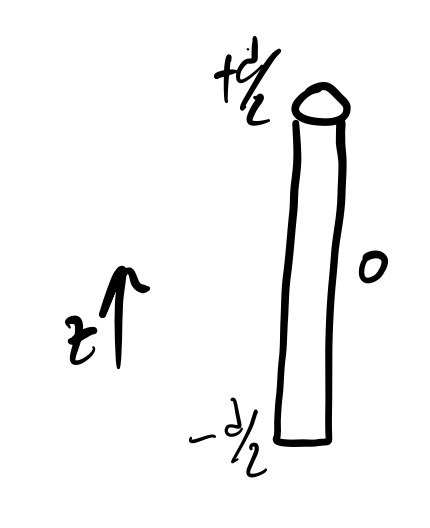
\includegraphics[scale=0.35]{Lectures/Images/lec11-antenna.png}
\end{center}

We can then consider the current density to be:
\begin{equation}
    \v{J}(\v{x}, t) = \hat{\v{z}}J(\v{x}, t) = \hat{z}\delta(x)\delta(y)I(z)e^{-i\omega t}
\end{equation}
With the current:
\begin{equation}
    I(z, t) = \int dxdy J(x, y, z, t)
\end{equation}
We now have the engineering choice for how to craft the current profile; so long as we choose the current to vanish at the edges, anything is ok. For example:

\begin{center}
    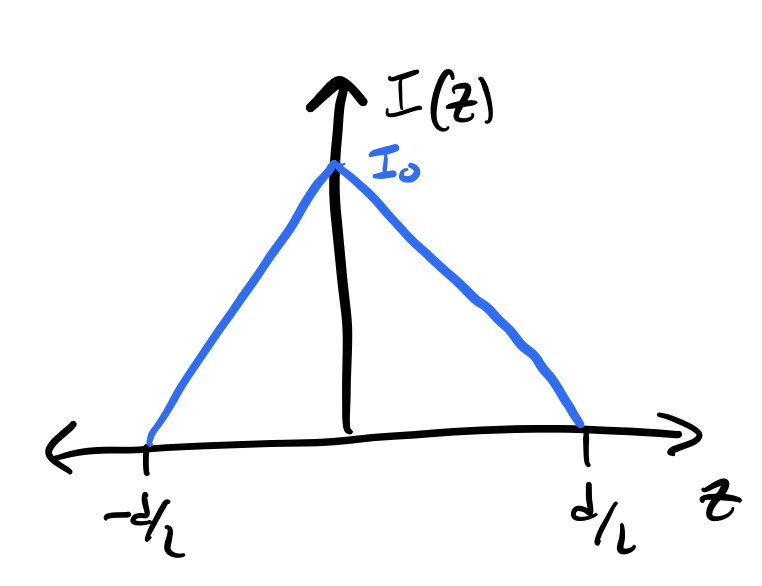
\includegraphics[scale=0.35]{Lectures/Images/lec11-antennacurrent.png}
\end{center}

where the above graphic describes:
\begin{equation}
    I(z) = I_0(1 - \frac{2\abs{z}}{d})
\end{equation}

we can now calculate the radiation from this antenna. We first calculate the $\rho'$:
\begin{equation}
    \rho'(z, t) = \int dxdy \rho(x, y, z, t)
\end{equation}
from the continuity equation:
\begin{equation}
    \dpd{}{t}\rho'(z, t) + \dpd{}{z}I(z, t) = 0 
\end{equation}
after we strip off the time dependence:
\begin{equation}
    \rho'(z) = \begin{cases}
        \frac{2iI_0}{\omega d} & 0 \leq z \leq d/2
        \\ -\frac{2iI_0}{\omega d} & -d/2 \leq z < 0
    \end{cases}
\end{equation}
There is a discontinuity at $z = 0$ as we feed current through the middle here in a non-differentiable way. In a real device the current we supply will be smooth. There is only a $z$-component to the dipole moment:
\begin{equation}
    p_z = \int_{-d/2}^{d/2}dz' z' \rho'(z') = \frac{iI_0d}{2\omega}
\end{equation}
\begin{equation}
    p_x = p_y = 0
\end{equation}
So then we have:
\begin{equation}
    \dod{P}{\Omega} = \frac{Z_0I_0^2}{128\pi^2}(kd)^2\sin^2\theta
\end{equation}
and:
\begin{equation}
    P = \frac{Z_0 I_0^2(kd)^2}{48\pi}
\end{equation}
which is the antenna analogue of the (non-relativistic) Larmor formula (non-relativistic as from our long-wavelength approximation, $\omega$ is small).

\emph{``I'm very happy that people are thinking... unusual experience for me, I guess''} - David Kutasov

\subsection{$j=1$: Antisymmetric/Magnetic Dipole Term}
Now we'll go to $j=1$\footnote{Going to be a long course... we'll be here in August going to $j = 3$. But more seriously, in some fields of physics people do go to very high orders of perturbation theory.}. From our power series formula:
\begin{equation}
    \v{A}(\v{x}) = \frac{\mu_0}{4\pi}\frac{e^{ikr}}{r}(-ik)\int d^3\v{x}'\v{J}(\v{x}')\hat{\v{n}}\cdot\v{\v{x}}'
\end{equation}
So $A_i$ involves $J_i \hat{n}_jx_j'$. It will be useful for us to split $J_ix_j'$ into a symmetric and antisymmetric part:
\begin{equation}
    J_ix_j' = \frac{1}{2}\underbrace{(J_ix_j' + J_jx_i')}_{(ij)} + \frac{1}{2}\underbrace{(J_ix_j' - J_jx_i')}_{[ij]}
\end{equation}
These two terms will have slightly different interpretations in terms of moments of the charge distribution. Let's look at the antisymmetric part first:
\begin{equation}
    J_ix_j' - J_jx_i' = \e_{ijk}(\v{J}\times \v{x}')_k
\end{equation}
Then:
\begin{equation}
    J_i \hat{n}_jx_j' \stackrel{\text{antisym}}{=} \left(\frac{1}{2}\hat{\v{n}} \times (\v{x}' \times \v{J})\right)_i
\end{equation}
Why is this interesting? The magnetic moment density enters the above expression:
\begin{equation}
    \v{M}(\v{x}) = \frac{1}{2}\v{x}\times\v{J}
\end{equation}
where the net magnetic moment is:
\begin{equation}
    \v{m} = \int d^3\v{x}\v{M}(\v{x})
\end{equation}
the bottom line is that the vector potential looks quite simple:
\begin{equation}
    \v{A}(\v{x}) = \frac{ik\mu_0}{4\pi}\hat{\v{n}}\times\v{m}\frac{e^{ikr}}{r}
\end{equation}
with associated magnetic/electric fields:
\begin{equation}
    \v{H} = \frac{1}{4\pi}k^2(\hat{\v{n}} \times \v{m})\times \hat{\v{n}}\frac{e^{ikr}}{r}
\end{equation}
\begin{equation}
    \v{E} = - \frac{Z_0}{4\pi}k^2\hat{\v{n}}\times \v{m}\frac{e^{ikr}}{r}
\end{equation}
so we see the same pattern where both the electric and magnetic fields are orthogonal to the direction of propagation of the wave.

One question we could ask is how is this related to the electric dipole story from earlier? You can read in Kutasov's notes how the two calculations are related by electromagnetic duality.

\subsection{$j=1$: Symmetric/Electric Quadrupole Term}
For the symmetric term, we are interested in the integral:
\begin{equation}
    \frac{1}{2}\int d^3\v{x}'\left[(\hat{\v{n}}\cdot\v{x}')\v{J}(\v{x}')+ (\hat{\v{n}}\cdot\v{J}(\v{x}'))\v{x}'\right]
\end{equation}
By the continuity equation, the above becomes:
\begin{equation}
    -\frac{i\omega}{2}\int d^3\v{x}'\v{x}'(\hat{\v{n}}\cdot\v{x}')\rho(\v{x}')
\end{equation}
From which we obtain:
\begin{equation}
    \v{A}(\v{x}) = -\frac{\mu_0ck^2}{8\pi}\frac{e^{ikr}}{r}\int d^3\v{x}'\v{x}'(\hat{\v{n}}\cdot\v{x}')\rho(\v{x}')
\end{equation}
qualitatively, it does indeed look like one higher moment of the charge distribution, with $\rho(\v{x}')$ giving the total charge/monopole term, $\v{x}'\rho(\v{x}')$ giving the dipole term, and $\v{x}'(\hat{\v{n}}\cdot\v{x}')\rho(\v{x}')$ giving the quadrupole term. The resulting magnetic/electric fields are given by:
\begin{equation}
    \v{H} = \frac{ik}{\mu_0}\hat{\v{n}} \times \v{A}
\end{equation}
\begin{equation}
    \v{E} = \frac{ik}{\mu_0}Z_0(\hat{\v{n}}\times\v{A})\times\hat{\v{n}}
\end{equation}
It is the now-familiar pattern of $\hat{\v{n}}, \v{H}, \v{E}$ being mutually orthogonal in the far-field limit. This will be the starting point of our discussion next time, where we will elaborate on the discussion of quadrapole moments. We could ask why do we care about these - in some situations it could be that not only the total charge/monopole term is zero, but also that the dipole moment also vanishes. In this case the quadrapole could be the leading contribution to the fields and thus to the radiation. In the problem set, you will see an example where this is indeed the case.
\section{Radiation from Continuous Sources III, Electromagnetic Fields in Media}

\subsection{Review}
We have been studying the radiation from a charge/current density:
\begin{equation}
    \begin{split}
        \v{J}(\v{x}, t) &= \v{J}(\v{x})e^{-i\omega t}
        \\ \rho(\v{x}, t) &= \rho(\v{x})e^{-i\omega t}
    \end{split}
\end{equation}
where $\omega = c\frac{2\pi}{\lambda}$ and the current/source is nonzero on length scale $d$. We expanded in $\frac{d}{\lambda} \ll 1$; the leading order approximation is the electric dipole contribution. The first subleading terms came in the form of the magnetic dipole and the electric quadrupole terms. The magnetic dipole fields looked like:
\begin{equation}
    \v{A}(\v{x}) = \frac{ik\mu_0}{4\pi}\hat{\v{n}}\times\v{m}\frac{e^{ikr}}{r}
\end{equation}
with the net magnetic moment defined as the integral of the magnetization density:
\begin{equation}
    \v{m} = \int d^3\v{x}\v{M}(\v{x})
\end{equation}
\begin{equation}
    \v{M}(\v{x}) = \frac{1}{2}\v{x} \times \v{J}
\end{equation}

\subsection{Electric Quadrupole Fields}
We arrived at the magnetic dipole/electric quadrupole term via the symmetric/antisymmetric decomposition:
\begin{equation}
    J^ix'^jn^j = \frac{1}{2}(J^i\hat{\v{n}}\cdot\v{x}' + x'^i\v{J} \cdot \hat{\v{n}}) + \text{a.s.}
\end{equation}
Let's now study the symmetric term appearing above to find the fields from the electric quadrupole:
\begin{equation}\label{eq:quadrupoleintegral}
    \frac{1}{2}\int d^3\v{x}'(\hat{\v{n}}\cdot\v{x}' \v{J} + (\hat{\v{n}}\cdot\v{J})\v{x}')
\end{equation}
Like last class, we can use the continuity equation to manipulate this integral:
\begin{equation}
    i\omega\rho(\v{x}) = \nabla \cdot \v{J}
\end{equation}
wherein the integral of Eq. \eqref{eq:quadrupoleintegral} becomes (after using the continuity equation and integrating by parts):
\begin{equation}
    \frac{1}{2}\int d^3\v{x}'\v{x}'(\hat{\v{n}}\cdot\v{x}')\rho(\v{x}')
\end{equation}
We then get an analogous formula to the (far zone) vector potential as we got for the magnetic dipole:
\begin{equation}
    \v{A}(\v{x}) = \frac{\mu_0 ck^2}{8\pi}\frac{e^{ikr}}{r}\int d^3\v{x}'\v{x}'(\hat{\v{n}}\cdot\v{x}')\rho(\v{x}')
\end{equation}
You can check that this is indeed subleading in $\frac{d}{\lambda}$ (compared to the electric dipole term). Computing the fields:
\begin{equation}
    \v{H} = \frac{ik}{\mu_0}\hat{\v{n}}\times\v{A} = -\frac{ick^3}{8\pi}\frac{e^{ikr}}{r}\int d^3\v{x}'(\hat{\v{n}}\times\v{x}')(\hat{\v{n}}\cdot \v{x}')\rho(\v{x}')
\end{equation}
\begin{equation}\label{eq:quadrapoleE}
    \v{E} = \frac{ik}{\mu_0}Z_0(\hat{\v{n}}\times\v{A})\times\hat{\v{n}}
\end{equation}
Note these have angular dependencies that differ from the electric fields, which you can check in your own time.

\subsection{Moments of a Charge Distribution \& the Quadrupole Tensor/Radiation}
\begin{itemize}
    \item First moment (electric monopole/total charge):
    \begin{equation}
        Q = \int d^3\v{x}\rho(\v{x})
    \end{equation}
    \item Second moment/first subleading moment (electric dipole):
    \begin{equation}
        \v{p} = \int d^3\v{x}\v{x}\rho(\v{x})
    \end{equation}
    which is of particle interest if the total charge is indeed zero, for example for a neutral atom. An example we can consider is the charge distribution sketched below:
    \begin{center}
        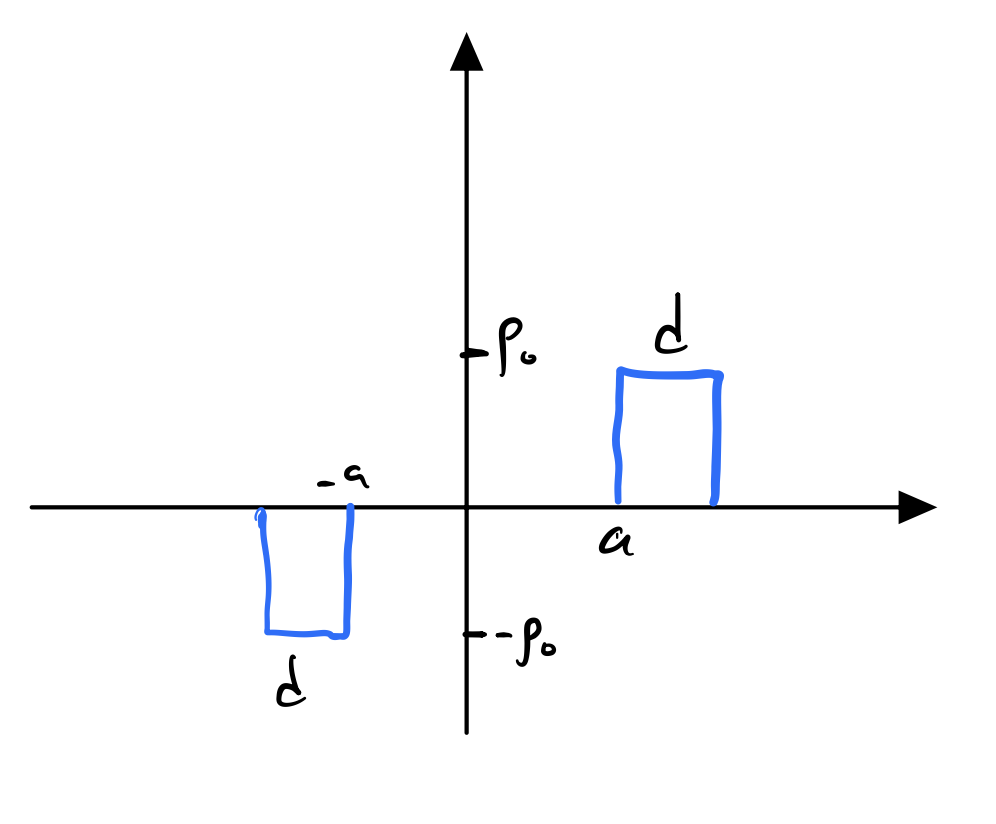
\includegraphics[scale=0.35]{Lectures/Images/lec12-dipoledchargedist.png}
    \end{center}
    where by inspection $Q = 0$, and for the dipole we find:
    \begin{equation}
        p_x = \int_{-\infty}^\infty = x\rho(x) = 2\int_{a}^{a+d}dx x\rho_0 = \rho_0\left[(a + d)^2 - a^2\right]
    \end{equation}
    This is the leading effect of the presence of this charge if we view this distribution from large distances.
    \item Third moment/Second subleading moment (electric quadrupole). Consider the tensor:
    \begin{equation}
        T_{ij} = \int d^3\v{x}x_ix_j\rho(\v{x})
    \end{equation}
    we note that $T_{ij}$ is manifestly symmetric. This has $\frac{3 \cdot 4}{2} = 6$ independent components. This is actually pretty interesting - $T_{ij}$ transforms as 5+1 dimensional object. This just means that the trace is rotationally invariant:
    \begin{equation}
        T_{ii} = \int d^3\v{x}\v{x}^2\rho(\v{x})
    \end{equation}
    the 5 then corresponds to the traceless and symmetric part of the matrix. In the $SU(2)$ language, this is the spin-2 representation (which has $2j + 1$ components), here we deal with $SO(3)$, but they are closely related. The traceless part we can write in the following way:
    \begin{equation}
        Q_{ij} = 3T_{ij} - \delta_{ij}T_{kk}
    \end{equation}
    The claim to fame of this object is that it is traceless:
    \begin{equation}
        Q_{ii} = 3T_{ii} - \delta_{ii}T_{kk} = 3T_{ii} - 3T_{kk} = 0
    \end{equation}
    How does this tensor help us? Going back to our integral that appeared in the quadrapole moment, we could write in index notation:
    \begin{equation}
        -\frac{i\omega}{2}\int d^3\v{x}' x_k'(\hat{n}_lx'_l)\rho(\v{x}')
    \end{equation}
    We can then write:
    \begin{equation}
        x_k'x_l' = \frac{1}{3}(3x_k'x_l' - \delta_{kl}\abs{\v{x}'}^2) + \frac{1}{3}\delta_{kl}\abs{\v{x}'}^2
    \end{equation}
    We note that the $\frac{1}{3}\delta_{kl}\abs{\v{x}'}^2$ term does not contribute to the fields, so we get\footnote{The 24 comes from the fact that famously $24 = 8\times3$}:
    \begin{equation}
        \v{H} = -\frac{ick^3}{24\pi}\frac{e^{ikr}}{r}\hat{\v{n}}\times Q\hat{\v{n}}
    \end{equation}
    where $Q$ is the 3x3 traceless symmetrix matrix $Q_{ij}$, and:
    \begin{equation}
        Q\hat{\v{n}} = Q_{ij}n_j
    \end{equation}
    We can then calculate the electric field $\v{E}$ from Eq. \eqref{eq:quadrapoleE}, and then from this calculate the differential power\footnote{I won't do the factorization of 1152 for you...}:
    \begin{equation}
        \dod{P}{\Omega} = \frac{c^2Z_0}{1152\pi^2}k^6\abs{(\hat{\v{n}} \times Q\hat{\v{n}}) \times \hat{\v{n}}}^2
    \end{equation}
    This tells us how much radiation is associated with the quadrapole moment of the distribution. If we integrate over all angles:
    \begin{equation}
        P = \frac{c^2Z_0k^6}{1440\pi}\frac{k^6}{\pi}\sum_{ij}^3\abs{Q_{ij}}^2
    \end{equation}
    this goes as $k^6$, while the dipole contribution goes as $k^4$. This is exactly as we expect - with each higher order moment we get one more power of $\frac{d}{\lambda}$ ($k$ - the $d$ is hiding in the moment) and hence in the power with each moment we get two more powers of $k$.
\end{itemize}

\subsection{Review - Electrostatics in Media}
Now we move back to Wald (Chapter 6) and discuss electrodynamics in media, e.g. the study of light waves propagating in water.
Last quarter you looked at electrostatics in media, but now we look at what changes in the dynamical case. But, since its been a while since you've had this discussion, let us review. 

Suppose we were in a non-vacuous media\footnote{I suppose air is technically a non-vacuous medium... certainly less violent than if the room was filled with honey. It would be quite difficult to breathe.}.There, there are notions of free charges and currents, as well as dipoles that may react to external fields and polarize the substance. It is also useful to average over a distance $L$ (not worry about the microscopics of the medium). Suppose $\psi$ is any physical quantity. We can then define the average as:
\begin{equation}
    \avg{\psi}(\v{x}) = \int d^3\v{x}' \psi(\v{x}')f_l(\v{x} - \v{x}')
\end{equation}
where $f_l(\v{x} - \v{x}')$ is a function that starts at 1 and drops off smoothly/quickly at length scale $L$.

\begin{center}
    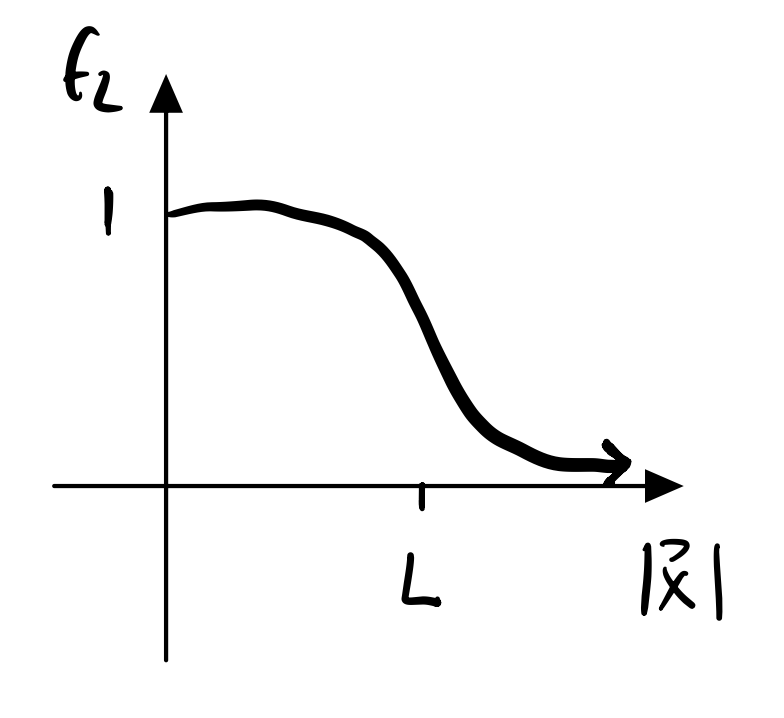
\includegraphics[scale=0.35]{Lectures/Images/lec12-fL.png}
\end{center}

We can look at the $\v{D}$-field in vacuum:
\begin{equation}
    \v{D}_{\text{vac}} = \e_0\v{E}_{\text{vac}}
\end{equation}
which we can average, anticipating that in matter we will want to coarse grain:
\begin{equation}
    \avg{\v{D}_{\text{vac}}} = \e_0\avg{\v{E}_{\text{vac}}}
\end{equation}
in matter we further add a polarization term:
\begin{equation}
    \avg{\v{D}} = \e_0\avg{\v{E}} + \avg{\v{P}}
\end{equation}
and there is an analogous expression for the $\v{H}$-field:
\begin{equation}
    \avg{\v{H}} = \frac{1}{\mu_0}\avg{\v{B}} - \avg{\v{M}}
\end{equation}

\subsection{Modifying Maxwell's Equations}
The first question we may ask is how we may modify Maxwell's equation now that we are inside a medium. The first thing to say is that Maxwell's equations are always true - so let's just start by writing them down again:
\begin{equation}\label{eq:Gauss}
    \nabla \cdot \v{E} = \frac{\rho}{\e_0}
\end{equation}
\begin{equation}\label{eq:Ampere}
    \nabla \times \v{B} - \frac{1}{c^2}\dot{\v{E}} = \mu_0 \v{J}
\end{equation}
\begin{equation}\label{eq:magneticGauss}
    \nabla \cdot \v{B} = 0
\end{equation}
\begin{equation}\label{eq:Faraday}
    \nabla \times \v{E} + \dot{\v{B}} = 0
\end{equation}
as we discussed when we studied the relativistically covariant version of the Maxwell equations, the source-free/Bianchi identity equations (Eqs. \eqref{eq:magneticGauss}, \eqref{eq:Faraday}) just become their averaged versions:
\begin{equation}
    \nabla \cdot \avg{\v{B}} = 0
\end{equation}
\begin{equation}
    \nabla \times \avg{\v{E}} + \avg{\dot{\v{B}}} = 0
\end{equation}
and further we remember from our discussion of electrostatics that Eq. \eqref{eq:Gauss} can be modified to be:
\begin{equation}
    \nabla \cdot \avg{\v{D}} = \avg{\rho_f}
\end{equation}
with $\rho_f$ the free charge density. The last equation Eq. \eqref{eq:Ampere} requires a little more consideration. Last quarter you saw that:
\begin{equation}
    \avg{J} \stackrel{\text{static}}{=} \avg{\v{J}_f} + \nabla \times \avg{\v{M}}
\end{equation}
but this is modified now to include a time derivative of the polarization:
\begin{equation}
    \avg{J} = \avg{\v{J}_f} + \nabla \times \avg{\v{M}} + \dpd{}{t}\avg{\v{P}}
\end{equation}
then combining this with:
\begin{equation}
    \avg{\v{H}} = \frac{1}{\mu_0}\avg{\v{B}} - \avg{\v{M}}
\end{equation}
we find the equivalent of Eq. \eqref{eq:Ampere}:
\begin{equation}
    \nabla \times \avg{\v{H}} - \dpd{}{t}\avg{\v{D}} = \avg{\v{J}_f}
\end{equation}
note the presence of the new $\p_t \avg{\v{D}}$ term! this was not important last quarter in electrostatics, but it is something we must consider here.

The situation is quite a bit subtle in the dynamic case. In the static case for example, there is no ambiguity about what are free charges - free charges are what can move in the presence of an external electric field, while the bound charges are those that do not move. So there is no mystery about what $\rho_f$ is. But here it is not obvious what $\rho_f$ is - how do we think about an electron that stays in the metal (but moves) in the presence of a sinusoidal field; is it free or bound? Really the issue is whether the microscopic charges contribute to $\rho_f$ or to the polarization $\v{P}$ (and a similar story with $\v{J}_f$ and $\v{M}$). There is an ambiguity, and we have to make sure we do not double count the contributions. This whole speech was to say that we need to break this ambiguity somehow - here we will take $\v{P}$ seriously.

Note that $\v{P}, \v{E}$ are not independent, and indeed the polarization depends on the electric field. Let us work in the limit where:
\begin{equation}
    \avg{\v{P}} \propto \avg{\v{E}}
\end{equation}
and so:
\begin{equation}
    \avg{\v{D}} = \e \avg{\v{E}}
\end{equation}
and similarly:
\begin{equation}
    \avg{\v{H}} = \frac{1}{\mu}\avg{\v{B}}
\end{equation}
What are $\e, \mu$? They are features of the material that we must measure. We will focus on how to modify this discussion in the dynamical case. What we've assumed - $\avg{\v{P}(t)} \propto \avg{\v{E}(t)}$ - doesn't quite make sense because it implies that the polarization at time $t$ reacts to the electric field at the same time $t$ instantaneously. For now, let us pretend it is correct in the sense that the variation of the electric field in time is slow (and so the material has time to react). Thus Maxwell's equations (with sources) can be written as:
\begin{equation}
    \nabla \cdot \avg{\v{E}} = \frac{1}{\e}\avg{\rho_f}
\end{equation}
\begin{equation}
    \nabla \times \avg{\v{B}} - \mu \e \avg{\dot{\v{E}}} = \mu\avg{\v{J}_f}
\end{equation}
These equations look the same as the equations in vacuum, just that we have replaced fields with their averages and have replaced $\e_0, \mu_0 \to \e, \mu$. We can define the index of refraction:
\begin{equation}
    n = \frac{\sqrt{\e\mu}}{\sqrt{\e_0\mu_0}}
\end{equation}
and if we go to the discussion in Wald chapter 5 and replace all $\e_0, \mu_0, c, \rho, \phi_f \to \e, \mu, c/n, \avg{\rho_f}, \avg{\phi_f}$, we will find EM waves propagating with speed $c/n$. In a little more detail, we can define a ``Lorenz gauge'':
\begin{equation}
    \frac{n^2}{c^2}\avg{\dot{\phi}} + \nabla \cdot \avg{\v{A}} = 0
\end{equation}
where in this gauge:
\begin{equation}
    \tilde{\square}\avg{\phi} = -\frac{1}{c}\avg{\rho_f}
\end{equation}
\begin{equation}
    \tilde{\square}\avg{\v{A}} = -\mu\avg{\v{J}_f}
\end{equation}
and:
\begin{equation}
    \tilde{\square} = -\frac{n^2}{c^2}\dpd[2]{}{t} + \nabla^2
\end{equation}
where $\frac{n^2}{c^2} = \frac{1}{c_{\text{mat}}^2}$.

A couple more comments - suppose the material we consider was infinite in extension. Then the waves propagate forever in the material. But any real material of course has a boundary. 

\begin{center}
    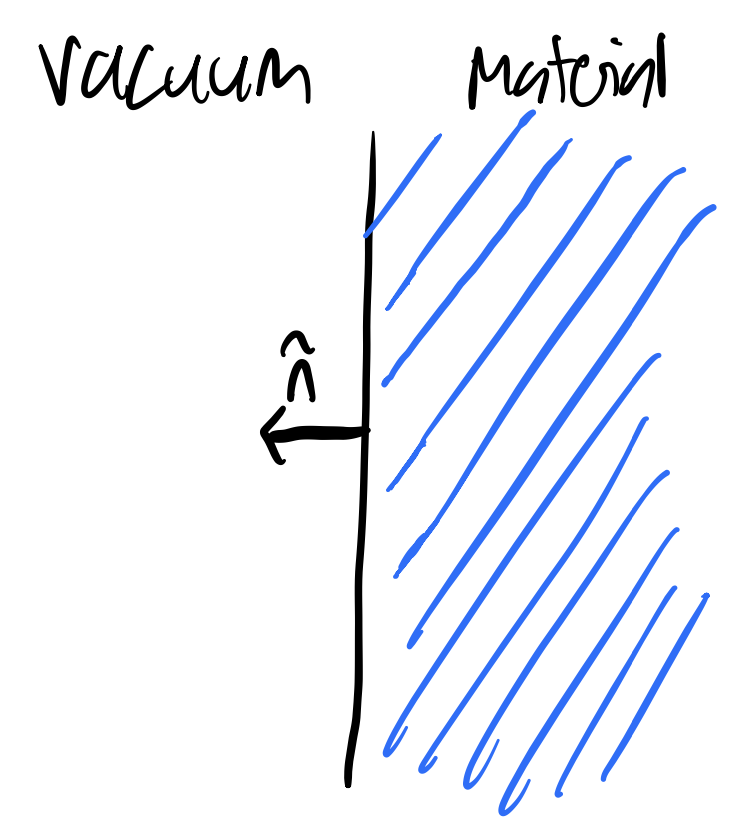
\includegraphics[scale=0.35]{Lectures/Images/lec12-interface.png}
\end{center}

We then have the boundary conditions:
\begin{itemize}
    \item $\avg{E_\parallel}, \hat{\v{n}}\cdot\avg{\v{B}}$ are continuous
    \item If there are no $\delta$-function contributions to $\avg{\rho_f}, \avg{\v{J}_f}$, then $\hat{\v{n}}\cdot\avg{\v{D}}, \avg{H_\parallel}$ are continuous.
\end{itemize}
Next week, you will study this scenario, and derive Snell's law on your problem set.

\end{document}